\documentclass[12pt,a4paper]{article} %12 кегль, формат бумаги А4, тип статья

\usepackage[T2A]{fontenc} %поддержка кириллицы
\usepackage[utf8]{inputenc} %кодировка символов юникод
\usepackage[english,russian]{babel} %список рабочих языков
\usepackage{cmap} %для поиска в pdf
\usepackage[left=2cm,right=2cm,top=2cm,bottom=2cm]{geometry} %размеры отступов от краев страницы
\usepackage{graphicx} %возможность работать с графикой
\usepackage{enumitem} %для работы со списками
\usepackage{float} %для точного размещения таблиц и графики
\usepackage{caption} %для создания подписей таблиц и графики
\usepackage{amsmath,amssymb,amsthm,amsfonts} %штуки для математики
\usepackage{extarrows} %чтобы подписи над и под нестандартными стрелками писать короче в коде
\usepackage{makeidx} %собирает ключевые слова для предметного указателя
\usepackage[hidelinks]{hyperref} %убирает выделение ссылок; добавляет гиперссылки в оглавление, перекрестные ссылки и URL
\usepackage{setspace} %устанавливает отступы
\linespread{1.5} %длина межстрочного интервала
\vspace{125mm} %длина абзацного отступа
\usepackage{titlesec}
\titleformat{\section}{\normalfont\Large\bfseries\centering}{}{0pt}{} % эти две строчки убирают циферки перед названиями разделов в основном тексте и выравнивают названия секций по центру
\usepackage{paratype} %чтобы точно был поиск и шрифт хороший

\author{Автор конспекта: Краснов Борис} %автор
\title{Белов Ю.С.: Комплексный анализ} %название
\date{Весна 2026} %дата создания документа

\newtheorem{theorem}{Теорема}
\newtheorem{lemma}{Лемма}
\newtheorem{definition}{Определение}
\newtheorem{proposition}{Предложение}
\newtheorem{consequence}{Следствие}
\newcommand{\R}{\mathbb{R}}
\newcommand{\Co}{\mathbb{C}}
\newcommand{\E}{\mathbb{E}}
\newcommand{\D}{\mathbb{D}}
\newcommand{\PR}{\mathbb{P}}
\newcommand{\charf}[2][t]{\varphi_{#2}(#1)}
\newcommand{\F}{\mathcal{F}}
\newcommand{\M}{\mathfrak{M}}

\begin{document}
	\maketitle
	\tableofcontents
	\clearpage
	\section{Что есть производная комплексной функции и учимся базовому интегрированию}
	\begin{definition}
		Функция $f:\Co\rightarrow\Co $ голоморфна в области(открытое, связное) $G\subset\Co$, если
		$$\forall z_0\in G\quad\exists\lim_{z\rightarrow z_0}\frac{f(z)-f(z_0)}{z-z_0}$$
	\end{definition}
	Нетрудно видеть, что для существования такого предела должны выполняться условия Коши-Римана:
	\begin{equation}\label{условиеК-Р}
		\begin{cases}
			\displaystyle\frac{\partial u}{\partial x}=\frac{\partial v}{\partial y}\\
			\displaystyle\frac{\partial u}{\partial y}=-\frac{\partial v}{\partial x}
		\end{cases}
	\end{equation}
	где $f(x+iy)=u(x,y)+iv(x,y)$.
	\begin{proof}
		$$\lim_{\varepsilon\rightarrow 0}\frac{f(z_0+\varepsilon)-f(z_0)}{\varepsilon}=\lim_{\varepsilon\rightarrow 0}\left[\frac{u(x_0+\varepsilon,y_0)-u(x_0,y_0)}{\varepsilon}+\frac{iv(x_0+\varepsilon,y_0)-iv(x_0,y_0)}{\varepsilon}\right]=$$ $$=\frac{\partial u(x_0,y_0)}{\partial x}+i\frac{\partial v(x_0,y_0)}{\partial y}$$
		$$\lim_{\varepsilon\rightarrow 0}\frac{f(z_0+i\varepsilon)-f(z_0)}{i\varepsilon}=\lim_{\varepsilon\rightarrow 0}\left[\frac{u(x_0,y_0+i\varepsilon)-u(x_0,y_0)}{i\varepsilon}+\frac{iv(x_0,y_0+i\varepsilon)-iv(x_0,y_0)}{i\varepsilon}\right]=$$ $$=-i\frac{\partial u(x_0,y_0)}{\partial x}+\frac{\partial v(x_0,y_0)}{\partial y}$$
	\end{proof}
	Распишем голоморфную функцию в терминах $o()$:
	$$f(z)=f(z_0)+f^{'}(z_0)(z-z_0)+o(|z-z_0|)$$\par
	Как мы знаем, дифференциал это линейное отображение, а в нашем случае это умножение на комплексное число $f^{'}(z_0)=re^{i\varphi}$, то есть оно еще и сохраняет углы, то есть поворотная гомотетия.
	\begin{definition}
		Функция $f:\Co\rightarrow\Co $ аналитическая в области $G\subset\Co$, если
		$$\forall z_0\in G\quad\exists B_R(z_0)\exists f(z)=\sum_{n=0}^{+\infty}c_n(z-z_0)^n,\quad |z-z_0|<R,\quad R>0$$
	\end{definition}
	Число $\sup R$ для фиксированного $z_0$ из определения называется радиусом сходимости ряда в точке $z_0$. При $|z-z_0|<R$ ряд сходится равномерно и абсолютно по критерию Вейерштрасса, вне области сходимости ряд соответственно расходится, а на границы ряд делает что хочет. Также коэффициенты в ряде Тейлора соответственно равны $\displaystyle c_n=\frac{f^{(n)}(z_0)}{n!}$.
	
	Лирическое отступление. Не трудно видеть, что аналитичные функции образуют алгебру над полем $\Co$. Также мы умеем искать первообразную у многочленов, а значит если мы возьмем произвольный замкнутый контур в области сходимости степенного ряда, то интеграл функции по нему будет 0. Если брать произвольный замкнутый контур в области $G$, то чтобы интеграл по нему был 0 достаточно, чтобы он содержался в ограниченной области и тогда в игру вступает определение компакта и представлений $f$ через степенные ряды будет конечное число раз, чтобы покрыть контур.
	
	\begin{proposition}\label{равнос для инт в круге}
		Пусть $f:\Co\rightarrow\Co$ непрерывна в области $G$, обладающей следующим свойством: $\exists z_0\in G:\forall z\in G$ можно дойти от $z_0$ передвигаясь только в направлении вещественной или мнимой оси(можно менять направления). Мы будем жить в круге с центром в 0. Тогда следующие условия эквивалентны ($\gamma$-кусочно-гладкий):
		\begin{enumerate}
			\item $\displaystyle\oint\limits_\gamma f(z)dz$ зависит только от концов $\gamma$;
			\item $\displaystyle\oint\limits_\gamma f(z)dz=0$ для произвольного замкнутого контура лежащего в $G$;
			\item у $f(z)$ существует первообразная, определенная на всей $G$;
			\item $\displaystyle\oint\limits_{\partial P} f(z)dz=0$ где $P$-смотреть картинку в доказательстве.
		\end{enumerate}
	\end{proposition}
	\begin{proof}
		\,
		\begin{enumerate}
			\item $1\Leftrightarrow 2$. Очевидно (не ленитесь, картиночку нарисуйте);
			\item $2\Rightarrow 4$ - без комментариев;
			\item $3\Rightarrow 2$. Параметризовали $\gamma$, записали интеграл, вспомнили, что контур замкнут и взяли разность двух равных чисел;
			\item $4\Rightarrow 3$. Положим кандидата на первообразную: $F(z)=\displaystyle\int_0^xf(s)ds+\int_x^{x+iy}f(s)ds$
			\begin{figure}[H]
				\centering
				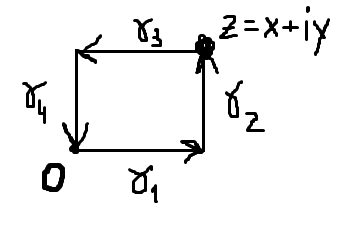
\includegraphics{im_proof_4eq.png}
				\caption{Картинка к док-ву}
			\end{figure}
			Теперь немного проверочек:
			$$\lim\limits_{\varepsilon\rightarrow 0}\frac{F(z+i\varepsilon)-F(z)}{i\varepsilon}=\lim\limits_{\varepsilon\rightarrow 0}\frac{1}{i\varepsilon}\int\limits_{[z,z+i\varepsilon]}f(s)ds=\lim\limits_{\varepsilon\rightarrow 0}\int_0^1f(z+it\varepsilon)dt=f(z)$$
			Заметим, что $\displaystyle\oint\limits_{\partial P} f(z)dz=0\Rightarrow F(z)=\int\limits_{\gamma_3}f(z)dz+\int\limits_{\gamma_4}f(z)dz$ откуда
			$$\lim\limits_{\varepsilon\rightarrow 0}\frac{F(z+\varepsilon)-F(z)}{\varepsilon}=\lim\limits_{\varepsilon\rightarrow 0}\frac{1}{\varepsilon}\int\limits_{[z,z+\varepsilon]}f(s)ds=f(z)$$
			Получили, что частные производные функции $F$, как отображения из $\R^2$ в $\R^2$, существуют и непрерывны(так как $f$ непрерывна), значит $F$ голоморфна, а так как совпадают с $f$, то производная $F$ равна $f$.
		\end{enumerate}
	\end{proof}
	\begin{theorem}
		$f$ голоморфна в круге $\Rightarrow \displaystyle\oint\limits_{\partial P}f(z)dz=0$ где $P$-прямоугольник в круге.
	\end{theorem}
	\begin{proof}
		Предположим, что это не так, тогда существует прямоугольник\\ $P:\displaystyle\oint\limits_{\partial P}f(z)dz=a\neq 0$.
		\begin{figure}[H]
			\centering
			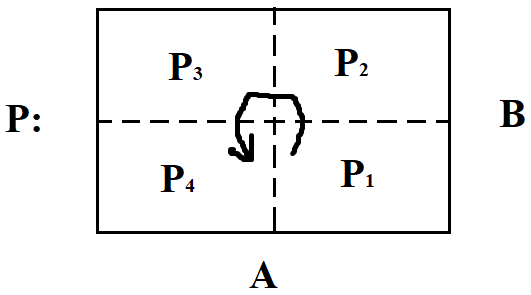
\includegraphics{im_proof_dif_int0.png}
			\caption{Картинка к док-ву}
		\end{figure}
		Тогда можно разбить прямоугольник на 4 равные части и получится следующая формула:
		$$\displaystyle\oint\limits_{\partial P}f(z)dz=\oint\limits_{\partial P_1}f(z)dz+\oint\limits_{\partial P_2}f(z)dz+\oint\limits_{\partial P_3}f(z)dz+\oint\limits_{\partial P_4}f(z)dz=a$$
		Из нее следует, что $\exists i\in \{1,2,3,4\}:\left|\displaystyle\oint\limits_{\partial P_i}f(z)dz\right|\geq\displaystyle\frac{|a|}{4}$.
		Обозначим этот прямоугольник за $P^{(1)}$, а исходный соответственно за $P^{(0)}$ со сторонами $A$ и $B$. Продолжим дробить выбранные прямоугольники, получая последовательность $\{P^{(n)}\}_{n=0}^{+\infty}$ со свойствами:\\ $\left|\displaystyle\oint\limits_{\partial P^{(n)}}f(z)dz\right|\geq\displaystyle\frac{|a|}{4^{n}}$, а также $\lim\limits_{n\rightarrow +\infty}P^{(n)}=z_0$. Тогда с одной стороны получаем:
		$$\left|\displaystyle\oint\limits_{\partial P^{(n)}}f(z)dz\right|=\left|\displaystyle\oint\limits_{\partial P^{(n)}}\left(f(z_0)+f^{'}(z_0)(z-z_0)+\varphi (z)\right)dz\right|=\left|\displaystyle\oint\limits_{\partial P^{(n)}}\varphi(z)dz\right|\geq\frac{|a|}{4^n},$$
		где $\varphi (z)=o(|z-z_0|)$, то есть $\varphi (z)\leq \varepsilon |z-z_0|$. А тогда
		$$\left|\displaystyle\oint\limits_{\partial P^{(n)}}\varphi(z)dz\right|\leq\frac{2A+2B}{2^n}\cdot\varepsilon\cdot\frac{A+B}{2^n}$$
		При этом стремление к нулю последней оценки быстрее, чем у $\frac{|a|}{4^n}$ ввиду произвольности $\varepsilon$.
	\end{proof}
	\begin{consequence}
		Теорема верна, если заменить прямоугольник на произвольный кусочно-гладкий замкнутый контур, лежащий в круге.
	\end{consequence}
	\begin{lemma}\label{лемма об устранимой особенности}
		(Об устранимой особенности). Рассмотрим круг $B$ с центром в $z_0$ и \\$f:\Co\rightarrow\Co$. Пусть $f\in C(B\setminus\{z_0\})$ и ограничена в $B\setminus\{z_0\}$. Если $\forall P\in B-\emph{прямоугольника}: z_0\notin P\quad\displaystyle\oint\limits_{\partial P}f(z)dz=0$, тогда $\forall P\in B-\emph{прямоугольника}\displaystyle\oint\limits_{\partial P}f(z)dz=0$.
	\end{lemma}
	\begin{proof}
		Заметим, что достаточно доказать для случая, когда особая точка попала на границу прямоугольника,
		так как если точка попала строго внутрь, то можно разбить прямоугольник на два с общей стороной, содержащей особую точку.
		\begin{figure}[H]
			\centering
			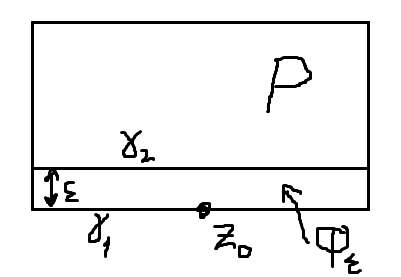
\includegraphics{im_lem_ustr_osob.png}
			\caption{Картинка к док-ву}
		\end{figure}
		$$\left|\displaystyle\oint\limits_{\partial P}f(z)dz\right|=\left|\oint\limits_{\partial \Phi_{\varepsilon}}f(z)dz\right|\leq C\varepsilon +\left|\int\limits_{\partial \gamma_1}f(z)dz+\int\limits_{\partial \gamma_2}f(z)dz\right|=C\varepsilon +\left|\int_a^b\left[f(t+i\varepsilon)-f(t)\right]dt\right|\underset{\varepsilon\rightarrow 0+}{\longrightarrow} 0$$
	\end{proof}
	\section{Голоморфность и аналитичность синонимы}
	\begin{theorem}\label{теорема Коши}
		(Малая интегральная формула Коши). Пусть $f(z)dz$ точная в $G$. Тогда для любого контура круга, обходимого один раз против часовой стрелки выполнено:
		\begin{equation}\label{формула_Коши}
			f(z)=\frac{1}{2\pi i}\oint\limits_{\gamma}\frac{f(w)}{w-z}dw
		\end{equation}
	\end{theorem}
	\begin{proof}
		\begin{figure}[H]
			\centering
			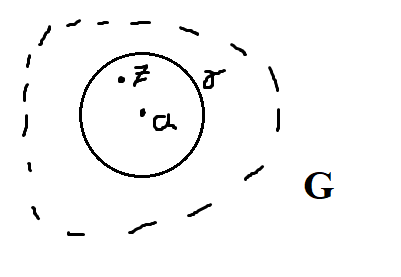
\includegraphics{im_proof_Kochi.png}
			\caption{Картинка к док-ву}
		\end{figure}
		Рассмотрим произвольную точку $a\in G$, произвольный $\overline{B_r(a)}\in G$ и произвольную точку $z\in B_r(a)$, а $\gamma=\partial B_r(a)$ соответственно. Рассмотрим $g(w)=\displaystyle\frac{f(z)-f(w)}{z-w}$. Она голоморфна и ограничена в нашем замкнутом круге(когда говорим о голоморфности в замкнутом множестве, имеем ввиду, что она голоморфна в области, содержащей наше замкнутое множество), кроме как в точке $w=z$. Тогда по лемме об устранимой особенности\eqref{лемма об устранимой особенности} $g(w)dw$ точна в круге. Тогда получаем:
		$$0=\oint\limits_{\gamma}g(w)dw=\oint\limits_{\gamma}\frac{f(z)-f(w)}{z-w}dw\Rightarrow$$
		$$\Rightarrow\oint\limits_{\gamma}\frac{f(w)}{z-w}dw=\oint\limits_{\gamma}\frac{f(z)}{z-w}dw=f(z)\oint\limits_{\gamma}\frac{dw}{z-w}$$
		Применим следующий фокус чтобы посчитать интеграл(интеграл равномерно сходящегося ряда - ряд интегралов)
		$$|w-a|>|z-a|\Rightarrow \frac{1}{z-w}=\frac{1}{(z-a)-(w-a)}=-\frac{1}{w-a}\cdot\frac{1}{1-\frac{z-a}{w-a}}=$$
		$$=\left\{\left|\frac{z-a}{w-a}\right|<1\right\}=-\sum_{n=0}^{+\infty}\frac{(z-a)^n}{(w-a)^{n+1}}$$
		\begin{equation*}
			\oint\limits_{\gamma}\frac{dw}{(w-a)^n}=
			\begin{cases}
				0,\quad n\neq 1\\
				2\pi i\quad n=1
			\end{cases}
		\end{equation*}
		Откуда $\displaystyle\oint\limits_{\gamma}\frac{dw}{z-w}=-2\pi i$.
		Тем самым $\displaystyle\oint\limits_{\gamma}\frac{f(w)dw}{z-w}=-2\pi if(z)$.
	\end{proof}
	\begin{consequence}
		(Теорема о среднем). Пусть $f$ аналитична в некотором круге с центром в $z$ и $\gamma$-граница круга, которую мы обходим против часовой стрелки один раз, тогда:
		$$f(z)=\frac{1}{2\pi i}\displaystyle\oint\limits_{\gamma}\frac{f(w)dw}{w-z}=\frac{1}{2\pi}\int_0^{2\pi}f(z+re^{it})dt,$$
		где $w=z+re^{it}$.
	\end{consequence}
	\begin{theorem}
		$f(z)dz$ точна в $G$. Тогда $f$ аналитична в $G$.
	\end{theorem}
	\begin{proof}
		Формула Коши\eqref{формула_Коши} из точности дает следующее:
		$$f(z)=\frac{1}{2\pi i}\oint\limits_{\gamma}\frac{f(w)dw}{w-z}=\sum_{n=0}^{+\infty}\frac{1}{2\pi i}\left[\oint\limits_{\gamma}\frac{f(w)dw}{(w-a)^{n+1}}\right](z-a)^n=\sum_{n=0}^{+\infty}c_n (z-a)^n,$$
		где $c_n=\displaystyle\frac{1}{2\pi i}\displaystyle\oint\limits_{\gamma}\frac{f(w)dw}{(w-a)^{n+1}}$ - новый способ вычислять коэффициенты в ряде Тейлора.
	\end{proof}
	\begin{theorem}
		Голоморфность функции в области равносильна ее аналитичности в той же области.
	\end{theorem}
	\begin{proof}
		Нетрудно видеть, что следует из предыдущих теорем.
	\end{proof}
	\begin{theorem}
		(Мореры) Следующие условия эквивалентны:
		\begin{enumerate}
			\item $f$ аналитична в $G$;
			\item $f$ голоморфна в $G$;
			\item $f(z)dz$ точна в $G$.
		\end{enumerate}
	\end{theorem}
	\begin{proof}
		Эквивалентность 1 и 2 доказали, как и следствие из 2 в 3. Осталось из 3 в куда-то, что делается так: форма точна, значит есть первообразная $F$, которая в свою очередь голоморфна, а значит аналитична и как следствие аналитична $f$.
	\end{proof}
	Замечание: в каждом пункте теоремы мы предъявляли разные требования для функции: принадлежность $C^{\infty}, C^1, C$ соответственно, а в итоге из них получаем "одинаковые свойства"\,функции - аналитичность.
	\section{Важная база теорем из формулы Коши}
	Лирическое отступление. Рассмотрим $f$-голоморфную функцию в области $G$. Мы знаем, что для нее выполняются условия Коши-Римана\eqref{условиеК-Р}, а также, что она аналитична. Тогда автоматически покомпонентные функции бесконечно гладкие и продиффиринцировав каждое равенство по $x$ и по $y$ получаем, что лапласиан покомпонентных функций равен 0. То есть из голоморфности $f$ следует, что покомпонентные части гармонические и сама функция тоже. 
	
	\begin{theorem}
		(Принцип максимума модуля) Пусть $f$ аналитична в $\overline{G}$. \\Тогда $\underset{\overline{G}}{\max}|f(z)|=\underset{\partial\overline{G}}{\max}|f(z)|$
	\end{theorem}
	\begin{proof}
		Случай строгого максимума. Если строгий максимум не на границе, тогда вокруг точки в которой он достигается, получаем противоречие с теоремой о среднем. Случай не строгого максимума. Если $\exists z_0\in G: |f(z_0)|=\underset{\partial\overline{G}}{\max}|f(z)|$, тогда по той же теореме о среднем функция локально постоянна, а как мы знаем, локально постоянная на связном есть константная.
	\end{proof}
	Поговорим о том, сколько достаточно знать об аналитической функции в области, чтобы восстановить ее.
	\begin{theorem}\label{т_единственности}
		(О единственности). Пусть $f$ и $g$ аналитичны в области $G$ и \\$\{\lambda_n\}_{n=0}^{+\infty}\in G: \lambda_n\rightarrow a\in G,\quad f(\lambda_n)=g(\lambda_n)$ и данная последовательность не стабилизирующаяся. Тогда $f\equiv g$ на $G$.
	\end{theorem}
	\begin{proof}
		Положим $h=f-g$. Из аналитичности $h(z)=\displaystyle\sum_{n=0}^{+\infty}c_n (z-a)^n$. Пусть $\exists c_{n_0}\neq 0$ и $n_0$ наименьшее такое. Тогда $h(z)=(z-a)^{n_0}\displaystyle\sum_{k=0}^{+\infty}c_{n_0+k}(z-a)^k=(z-a)^{n_0}\widehat{h}(z)$ и получаем $h(\lambda_n)=0\Rightarrow \widehat{h}(\lambda_n)=0\Rightarrow\widehat{h}(a)=0$ -противоречие с тем, что $c_{n_0}\neq 0$.
	\end{proof}
	\begin{consequence}
		Если функция $f\not\equiv 0$ аналитична в некоторой области $G$ и $K$ некоторый компакт в этой области, тогда $f$ имеет конечное число нулей в $K$.
	\end{consequence}
	\begin{proof}
		Если число нулей бесконечно, тогда можно выбрать сходящуюся оследовательность нулей и значит функция тождественный нуль.
	\end{proof}
	\begin{definition}
		Целая функция - функция аналитичная на всей $\Co$.
	\end{definition}
	\begin{theorem}
		(Лиувилля) Пусть $F$ целая и ограниченная функция. Тогда она константная.
	\end{theorem}
	\begin{proof}
		Как мы знаем:
		$$F(z)=\displaystyle\sum_{n=0}^{+\infty}c_nz^n,\quad c_n=\frac{1}{2\pi i}\oint\limits_{\gamma}\frac{F(w)dw}{w^{n+1}}$$
		Пусть $r$ радиус окружности по которой мы будем интегрировать, тогда:
		$$|c_n|\leq \frac{1}{2\pi}\cdot\underset{r=|z|}{\max}|F(z)|\cdot 2\pi r\frac{1}{r^{n+1}}=\frac{\underset{r=|z|}{\max}|F(z)|}{r^n}\leq \frac{C}{r^n}$$
	\end{proof}
	\begin{proposition}
		Пусть $F$ целая функция. Обозначим за $M_F(r)=\underset{r=|z|}{\max}|F(z)|$. Пусть $M_F(r)\leq Cr^n$. Тогда $F$ полином степени не выше $n$.
	\end{proposition}
	\begin{proof}
		Оценить коэффициенты в ряде Тейлора, как в доказательстве т. Лиувилля.
	\end{proof}
	А теперь самое лучше доказательство ОТА, которое нам показывали до этого момента.
	\begin{proof}
		$$p(z)=\displaystyle\sum_{i=0}^na_i z^i=a_n z^n\left(1+\sum_{i=0}^{n-1}\displaystyle\frac{a_i}{a_n}\cdot\displaystyle\frac{1}{z^{n-i}}\right)$$
		Достаточно далеко от 0:
		$$|p(z)|\geq |a_n||z|^n\left(1-\displaystyle\sum_{i=0}^{n-1}\displaystyle\frac{|a_i|}{|a_n|}\cdot\displaystyle\frac{1}{|z|^{n-i}}\right)\geq \displaystyle\frac{|a_n|}{2}|z|^n$$
		Тем самым получаем, что $\displaystyle\frac{1}{p(z)}$ ограничена. Если предположить, что корней нет, то тогда она еще и целая, а тогда по теореме Лиувилля исходный многочлен равен константе.
	\end{proof}
	\section{Понятие регулярных ветвей}
	Лирическое отступление о том, как задавать область аналитичности функции, о том как функции аналитически продолжать. Рассмотрим $f(w)=w^2$. Мы хотим однозначно решать уравнение $f(w)=z$. Для квадратного корня положим $\sqrt{z}=\sqrt{r}e^{i\frac{\varphi}{2}}$, где $r=|z|, -\pi<\varphi\leq\pi$. Тем самым область решения в данном случае - комплексная плоскость без действительной прямой $x\leq 0$. Простой проверкой по определению можем заключить, что в этой области корень дифференцируем, а именно:
	$$\displaystyle\lim\limits_{z\rightarrow z_0}\displaystyle\frac{\sqrt{z}-\sqrt{z_0}}{z-z_0}=\lim\limits_{z\rightarrow z_0}\displaystyle\frac{(\sqrt{z}-\sqrt{z_0})(\sqrt{z}+\sqrt{z_0})}{(z-z_0)(\sqrt{z}+\sqrt{z_0})}=\dfrac{1}{2\sqrt{z_0}}$$
	Заметим, что нам ничего не мешает продолжать область определения корня через особую прямую, просто тогда областью определения будет двулистное накрытие плоскости или по умному риманова поверхность.
	\begin{figure}[H]
		\centering
		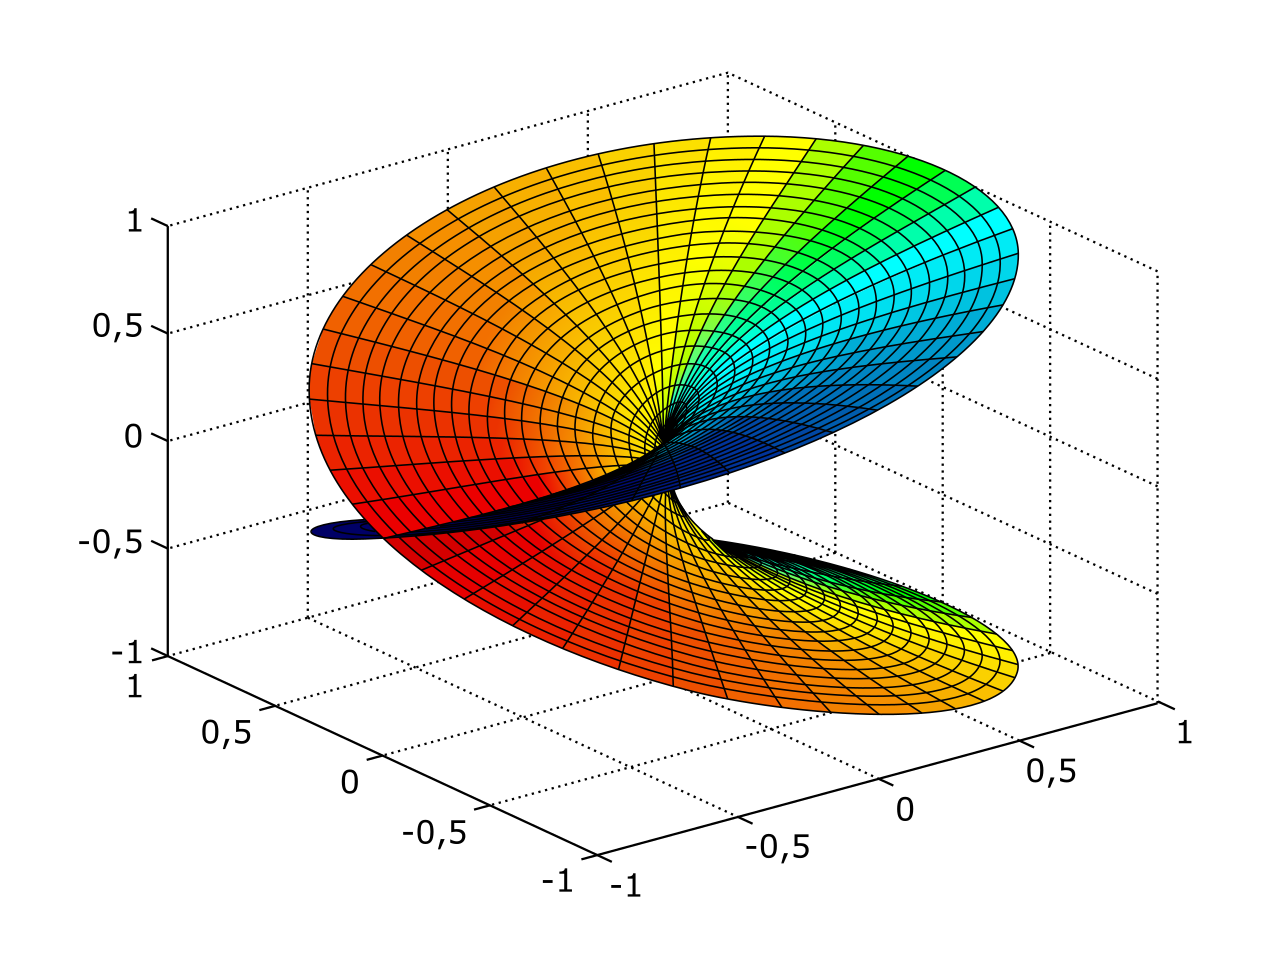
\includegraphics[scale=0.2]{Riemann_sqrt.svg.png}
		\caption{$f(z)=\sqrt{z}$}
	\end{figure}
	\begin{figure}[H]
		\centering
		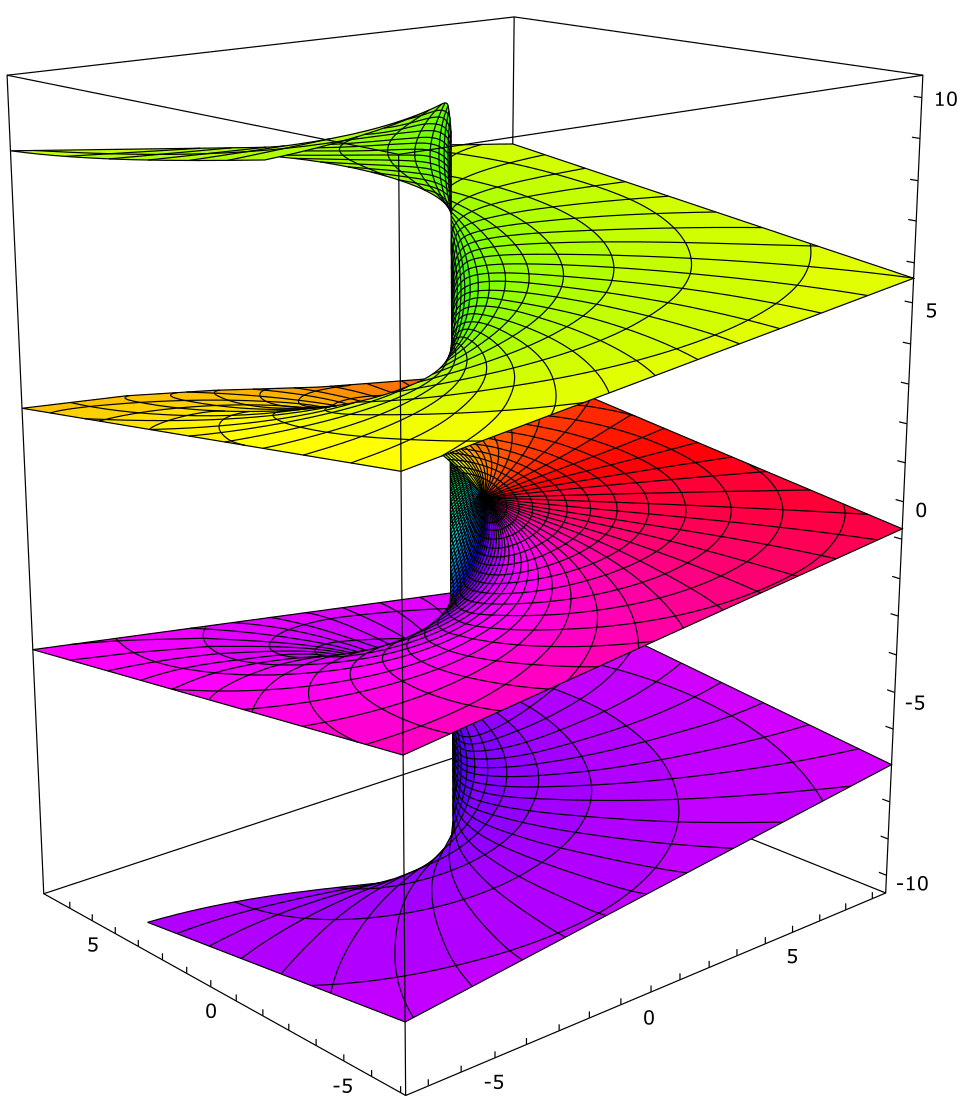
\includegraphics[scale=0.2]{Riemann_surface_log.svg.png}
		\caption{$f(z)=\log z$}
	\end{figure}
	Вообще это все было к тому, что за область жизни комплексных функций удобно брать не комплексную плоскость, а так называемую риманову поверхность - одномерное гладкое комплексное многообразие. Главная идея - каждой точке поверхности соответсвует единственное значение функции и при непрерывном перемещении по поверхности, значение функции непрерывно меняется.
	\section{Гомотопные контура, ряд Лорана, классификация особенностей}
	Сделаем некоторое обобщение предложения\eqref{равнос для инт в круге}.
	\begin{theorem}
		Пусть $f$ голоморфна в области $G$, $\gamma_1$ и $\gamma_2$ гомотопные пути в $G$. Тогда выполнено
		$$\displaystyle\int\limits_{\gamma_1}f(z)dz=\int\limits_{\gamma_2}f(z)dz$$
	\end{theorem}
	\begin{proof}
		\begin{figure}[H]
			\centering
			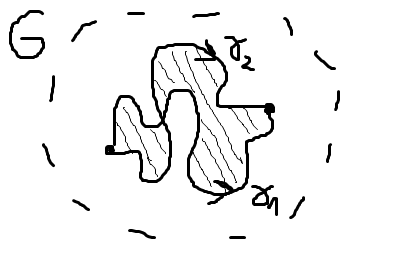
\includegraphics{гомотопные_пути.png}
			\caption{Образ гомотопии}
		\end{figure}
		Для начала, гомотопия это непрерывное отображение прямоугольника-компакта, то есть образ компакт. Тогда можно образ покрыть конечным набором открытых шаров $\{B_i\}_{i=1}^n$, лежащих в $G$. По теореме Кантора можем взять общий $\varepsilon$, такой что любой открытый круг в прямоугольнике и в образе радиуса $\varepsilon$ лежит целиком в каком-то $B_i$. Разобьем прямоугольник на сетку из прямоугольников целиком лежащих в кругах с радиусом $\varepsilon$.
		\begin{figure}[H]
			\centering
			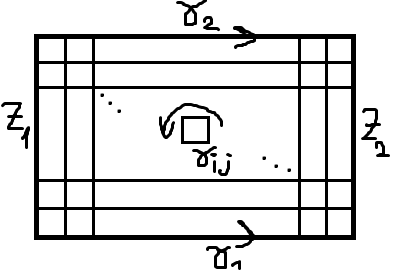
\includegraphics{гомотопия.png}
			\caption{Разбиение прямоугольника гомотопии(обозначения на рисунке относятся к образам подписанных частей)}
		\end{figure}
		Так как образы маленьких прямоугольников лежат в кругах, в которых функция голоморфна, то интеграл по образу границы маленького прямоугольника равен 0. Тогда можно написать следующее равенство:
		$$0=\displaystyle\sum_{i=1}^N\sum_{j=1}^M\oint\limits_{\gamma_{i,j}}f(z)dz=\oint\limits_{\gamma_1}f(z)dz-\oint\limits_{\gamma_2}f(z)dz$$
		Как видно из картинки, сумма интегралов по образам границ маленьких прямоугольников убивает интегрирование по внутренней сетке и добавляет интегралы по нашим путям, а также есть две части, где мы интегрируем по образам вертикальных границ, но так как их образы это точки начала и конца путей, то по ним интеграл 0.
	\end{proof}
	\begin{consequence}
		В односвязной области интеграл голоморфной функции по замкнутому контуру равен 0.
	\end{consequence}
	\begin{consequence}
		Формула Коши\eqref{формула_Коши} верна, если контур гомотопен тривиальному пути, так как окружность ему гомотопна.
	\end{consequence}
	Теперь поговорим о том, что делать если в области аналитичности функции есть особенность. Оказывается, что тогда функция тоже раскладывается в ряд, только там есть и обратные степени, а также по виду это ряда можно классифицировать эти особенности.
	\begin{theorem}
		Пусть функция $f$ голоморфна в открытом кольце $A_{r,R}$ с центром в $a$ и $z\in A_{r,R}$. Тогда функция раскладывается в ряд Лорана:
		$$f(z)=\displaystyle\sum_{n\in\mathbb{Z}}c_n (z-a)^n$$
		Сумма с отрицательными степенями называется главной частью, а остальная часть называется аналитической.
	\end{theorem}
	\begin{proof}
		Положим $\gamma_1: |z|=r+\varepsilon$ и $\gamma_2: |z|=R-\varepsilon$, а также соеденим их взаимнообратными путями $\gamma^-,\gamma^+$. Положим за $\gamma=\gamma^+\cup\gamma_2\cup\gamma^-\cup\gamma_1$.
		\begin{figure}[H]
			\centering
			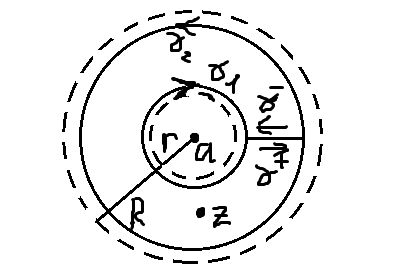
\includegraphics{для_ряда_Лорана.png}
			\caption{Картинка к док-ву}
		\end{figure}
		Это замкнутый контур, который гомотопен тривиальному пути, а значит верна теорема Коши:
		$$2\pi i\cdot f(z)=\displaystyle\oint\limits_{\gamma}\frac{f(w)dw}{w-z}=\oint\limits_{\gamma_1}\frac{f(w)dw}{w-z}+\oint\limits_{\gamma_2}\frac{f(w)dw}{w-z}$$
		Вспомним, как мы раскладывали в ряд $\displaystyle\frac{1}{w-z}$ в доказательстве теоремы Коши и сделаем здесь также, только контуров два и разложения будут разные.
		$$\frac{1}{w-z}=\displaystyle\sum_{n=0}^{+\infty}\frac{(z-a)^n}{(w-a)^{n+1}}\quad |w-a|=R-\varepsilon$$
		$$\frac{1}{w-z}=-\displaystyle\sum_{n=0}^{+\infty}\frac{(w-a)^n}{(z-a)^{n+1}}\quad |w-a|=r+\varepsilon$$
		Тогда получаем следующее разложение в ряд Лорана:
		$$f(z)=\displaystyle\sum_{n=0}^{+\infty}\frac{1}{2\pi i}\left[\oint\limits_{\gamma_1}\frac{f(w)dw}{(w-a)^{n+1}}\right](z-a)^n-\sum_{n=-\infty}^{-1} \frac{1}{2\pi i}\left[\oint\limits_{\gamma_2}f(w)(w-a)^{-n+1}dw\right](z-a)^n$$
		И бонусом получаем формулу для вычисления коэффициентов в ряде Лорана.
	\end{proof}
	Теперь можем классифицировать особенности. Пусть $f$ голоморфна в шаре без точки $B\setminus\{a\}$.
	\begin{definition}
		\,
		\begin{enumerate}
			\item Устранимая особенность: $f$ ограничена в окрестности $a$;
			\item Полюс: $\underset{z\rightarrow a}{\lim}|f(z)|=+\infty$;
			\item Существенная особенность: $\nexists\,\underset{z\rightarrow a}{\lim}|f(z)|$.
		\end{enumerate}
	\end{definition}
	Примеры:
	\begin{enumerate}
		\item $z^3$, просто определим в 0 как угодно;
		\item $\displaystyle\frac{1}{z^2}$;
		\item $e^{\frac{1}{z}}$, так как по мнимой оси нет предела.
	\end{enumerate}
	\begin{theorem}
		Классификация особенностей через вид главной части ряда Лорана:
		\begin{enumerate}
			\item $a$-устранимая особенность $\Longleftrightarrow$ $f$ аналитична в $a$;
			\item $a$-полюс $\Longleftrightarrow$ главная часть в разложении в $a$ состоит из конечного числа слагаемых;
			\item $a$-существенная особенность $\Longleftrightarrow$ главная часть в разложении в $a$ состоит из безконечного числа слагаемых.
		\end{enumerate}
	\end{theorem}
	\begin{proof}
		\,
		\begin{enumerate}
			\item По лемме об устранимой особенности в одну сторону и очевидно в другую сторону.
			\item Рассмотрим $g(z)=\displaystyle\frac{1}{f(z)}$. Она аналитична в окрестности $a$, которая является устранимой особенностью и значит имеет место
			$$g(z)=\displaystyle\sum_{n=0}^{+\infty}d_n(z-a)^n=d_k(z-a)^k+\sum_{n=k+1}^{+\infty}d_k(z-a)^n,$$
			где $d_k$ первый ненулевой коэффициент и соответственно кратность 0 $g(z)$ в $a$ равна $k$. То есть:
			$$|g(z)|=(1+o(1))|z-a|^k\quad z\rightarrow a$$
			Откуда получаем, что коэффициенты $f$ в ряде Лорана в точке $a$ с номером меньшим чем $-k$ равны 0:
			$$|f(z)|\leq C|z-a|^k\Rightarrow$$
			$$|c_{-n}|=\left|\displaystyle\frac{1}{2\pi i}\oint\limits_{\gamma_{\varepsilon}}f(w)(w-a)^{n+1}\right|\underset{\varepsilon\rightarrow 0}{\longrightarrow}0,$$
			где $\gamma_{\varepsilon}$ окружность вокруг $a$ радиуса $\varepsilon$. В обратную сторону: так как в главной части конечное число членов, то есть с минимальным номером, который будет стремиться к бесконечности быстрее остальных.
			\item За бесплатно получили из первых двух утверждений.
		\end{enumerate}
	\end{proof}
	\begin{definition}
		Если особая точка функции является полюсом, то его кратностью называется число, равное наименьшему номеру ненулевого коэффициента в ряде Лорана функции в этой точке, взятого со знаком минус ($k$ из доказательства выше).
	\end{definition}
	\begin{definition}
		Функция называется мероморфной в области $G$, если все особенности в этой области являются полюсами, а вне их она голоморфна.
	\end{definition}
	\begin{figure}[H]
		\centering
		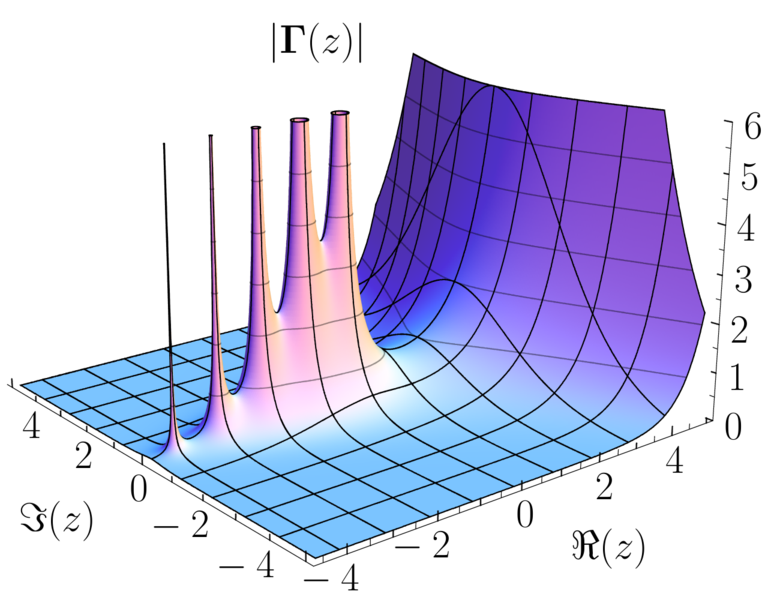
\includegraphics[scale=0.2]{gamma_function.png}
		\caption{Гамма функция мероморфна на всей плоскости}
	\end{figure}\par
	Заметим, что у мероморфной функции полюса изолированы, то есть не существует не стабилизируещейся последовательности полюсов в мероморфной области, сходящейся к полюсу в той же области, так как тогда можно было бы домножить функцию на моном $(z-z_0)^p$, где $z_0$ предельный полюс, а $p$ его кратность. Тогда в $z_0$ функция будет принимать какое-то комплексное значение, а в полюсах, которые сходились к $z_0$ все также бесконечность и тут слегка противоречие с непрерывностью.
	\section{Вычеты}
	Теперь поговорим о том, как считать интегралы в вычетах (теперь интеграл буквально сумма). Пусть у функции есть особенность в точке и мы хотим посчитать интеграл по окружности вокруг этой точки, а внутри круга функция голоморфна. Тогда мы можем записать функцию в ряд Лорана в этой точке и интегралы от всех слагаемых, кроме одного будут 0.
	$$\displaystyle\oint\limits_{\gamma}f(z)dz=2\pi i c_{-1}$$
	\begin{definition}
		Если функция $f$ в аналитичной области имеет особую точку $a$, то будем называть вычетом $f$ в $a$ число $Res_a f$, равное коэффициенту в ряде Лорана $f$ в $a$ при $\displaystyle\frac{1}{z-a}$.
	\end{definition}
	\begin{theorem}
		(Теорема о вычетах) Пусть $f$ аналитична в $G\setminus\{a_1,\cdots,a_n\}$, $G$ односвязна. Пусть $\gamma$ некоторая петля в $G$, такая что $Ind_{a_k}\gamma=1\quad\forall k\in\overline{1,n}$. Тогда имеет место следующее равенство:
		$$\displaystyle\oint\limits_{\gamma}f(z)dz=2\pi i\cdot\sum_{i=1}^nRes_{a_i}f$$
	\end{theorem}
	\begin{proof}
		На картинке показано, что мы берем около каждой особой точки окружность, не пересекающую другие особые точки и лежащую в области и соединяем ее какой-то кривой с исходной петлей.
		\begin{figure}[H]
			\centering
			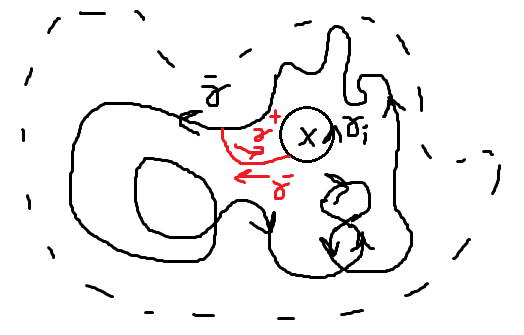
\includegraphics{теорема_о_вычетах.png}
			\caption{Картинка к док-ву}
		\end{figure}
		Опять берем и объединяем в единый контур все кривульки и он будет гомотопен тривиальному пути, а значит по нему интеграл 0, откуда:
		$$0=\displaystyle\oint\limits_{\cup\gamma}f(z)dz=\oint\limits_{\gamma}f(z)dz-\sum_{i=1}^n\oint\limits_{\gamma_i}f(z)dz=\oint\limits_{\gamma}f(z)dz-2\pi i\cdot\sum_{i=1}^nRes_{a_i}f$$
		Моя попытка в строгость. Нарисовать окружности можем, так как особые точки внутри области(открытое, связное)  отделимы, так как их конечное число. Соеденить петлю с окружностями можем, так как связность. А односвязность нужна, чтобы не было случая типо картинки в ряде Лорана - кольцо, в котором есть особая точка и петля это окружность посередине кольца, то есть чтобы не было у нас других особых точек, кроме названных. Тем самым что-то вроде той картинки нарисовать получилось. Объединение кривых есть кривая, гомотопная тривиальной петле (к сожалению я не могу строго объяснить почему есть такая гомотопия, кроме как нарисовать удобную картинку и подвигать кривульку ручками (Панина учила двигать ручками, либо линейная гомотопия и тут оба способа меня не устраивают, а по другому меня не учили, цитата у всех общая: "формулу написать не берусь")).
	\end{proof}
	Примеры вычисления вещественного интеграла в вычетах:
	$$\displaystyle\int\limits_{\R}\frac{\cos x}{1+x^2}dx=\int\limits_{\R}\frac{e^{ix}}{1+x^2}dx=$$
	(так как мнимая часть с синусом умрет, из-за того что интеграл вещественный)
	$$=\underset{R\rightarrow +\infty}{\lim}\int_R^R\frac{e^{ix}}{1+x^2}dx=\underset{R\rightarrow +\infty}{\lim}\left[\int\limits_{\gamma_R}\frac{e^{iz}}{1+z^2}dz-\int\limits_{\frown}\frac{e^{iz}}{1+z^2}dz\right]=2\pi i\cdot Res_if=\frac{\pi}{e}$$
	\begin{figure}[H]
		\centering
		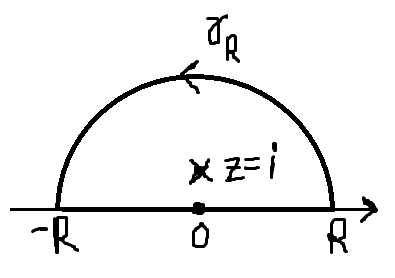
\includegraphics{счет_в_вычетах.png}
		\caption{Картинка к вычислению}
	\end{figure}
	$$\left|\displaystyle\int\limits_{R=|z|}\frac{e^{iz}}{1+z^2}dz\right|\leq \frac{2\pi R}{R^2-1}\underset{R\rightarrow +\infty}{\longrightarrow}0$$
	Второй пример:
	$$\displaystyle\int_0^{+\infty}\frac{\sin x}{x}dx=\frac{1}{2}\int\limits_{\R}\frac{\sin x}{x}dx=\frac{1}{2i}\int\limits_{\R}\frac{e^{iz}}{z}dz=\lim_{\substack{\varepsilon\rightarrow 0+ \\ R\rightarrow +\infty}}\int\limits_{\varepsilon<|x|<R}\frac{e^{iz}}{z}dz=$$
	$$=\lim_{\substack{\varepsilon\rightarrow 0+ \\ R\rightarrow +\infty}}\left[\int\limits_{\gamma_{\varepsilon,R}}\frac{e^{iz}}{z}dz-\int\limits_{\gamma_{\varepsilon}}\frac{e^{iz}}{z}dz-\int\limits_{\gamma_R}\frac{e^{iz}}{z}dz\right]=-\underset{\varepsilon\rightarrow 0+}{\lim}\int\limits_{\gamma_{\varepsilon}}\frac{e^{iz}}{z}dz-\underset{R\rightarrow +\infty}{\lim}\int\limits_{\gamma_R}\frac{e^{iz}}{z}dz$$
	\begin{figure}[H]
		\centering
		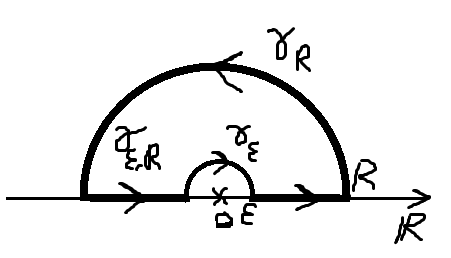
\includegraphics{Второй_пример_выч.png}
		\caption{Картинка к вычислению}
	\end{figure}
	$$\left|\int\limits_{\gamma_R}\frac{e^{iz}}{z}dz\right|=\left|\int_0^{\pi}\frac{e^{iRe^{it}}}{Re^{it}}dRe^{it}\right|\leq$$
	$$\leq \left|\int_0^{\frac{1}{\sqrt{R}}}e^{iR\cos t}\cdot e^{-R\sin t}dt\right|+\left|\int_{\frac{1}{\sqrt{R}}}^{\pi-\frac{1}{\sqrt{R}}}e^{iR\cos t}\cdot e^{-R\sin t}dt\right|+\left|\int_{\pi-\frac{1}{\sqrt{R}}}^{\pi}e^{iR\cos t}\cdot e^{-R\sin t}dt\right|\leq$$
	$$\leq \frac{2}{\sqrt{R}}+\pi\cdot e^{-R\sin \frac{1}{\sqrt{R}}}\underset{R\rightarrow +\infty}{\longrightarrow} 0$$
	$$\int\limits_{\gamma_{\varepsilon}}\frac{e^{iz}}{z}dz=\int\limits_{\gamma_{\varepsilon}}\frac{dz}{z}+\int\limits_{\gamma_{\varepsilon}}\frac{e^{iz}-1}{z}dz=\int\limits_{\gamma_{\varepsilon}}\frac{dz}{z}=-\pi i$$
	Так как $\frac{e^{iz}-1}{z}$ целая (ряд напишите).
	Откуда получаем:
	$$\int_0^{+\infty}\frac{\sin x}{x}dx=\frac{\pi}{2}$$
	\section{Пикар и Сохоцкий}
	% Пикара оставили
	\begin{theorem}
		(Пикара) Пусть в точке $a$ существенная особенность и
		\begin{enumerate}
			\item $f$ аналитична в проколотой окрестности $a$ - $U$
			\item $f$ мероморфна в проколотой окрестности $a$ - $U$
		\end{enumerate}
		Тогда для любой окрестности $a$ - $V\subset U$ верно, что
		\begin{enumerate}
			\item $f(V)=\Co$ или $f(V)=\Co\setminus\{p\}$
			\item $f(V)=\Co\cup\{\infty\}\setminus\{p_1,p_2\}$
		\end{enumerate}
	\end{theorem}
	\begin{proof}
		Хозяин сказал без док-ва $\rangle:<\quad \langle:($
	\end{proof}
	\begin{theorem}
		(Сохоцкого) Пусть у мероморфной в проколотой окрестности точки $a$ существенная особенность. Тогда для любой окрестности $a$ ее образ плотен в $\Co$.
	\end{theorem}
	\begin{proof}
		Пусть $U$ окрестность $a$ и пусть нашлось $B_{b}(r)$, которое имеет пустое пересечение с образом $U$. Тогда $h(z)=\displaystyle\frac{1}{f(z)-b}$ ограничена в $U$ и аналитична там, кроме как в $a$. Но по лемме об устранимой особенности $h$ аналитична и в $a$, а значит \\$f(z)=\displaystyle\frac{1}{h(z)}+b$ не имеет существенной особенности в $a$ - противоречие.
	\end{proof}
	\section{Принцип аргумента и связанное}
	Теперь поговорим о том, что такое логарифм аналитической функции. Легко сказать, что такое $\log z$ для $z=re^{i\varphi}$, так как можно просто положить $\log z=\log r + i\varphi$ и опять функция определена везде, кроме неположительной вещественной оси, но и это дело поправимое, просто логарифм будет жить на бесконечнолистном накрытии плосткости, кроме точки 0 (картинка ранее была). Так просто сказать, что такое логарифм произвольной аналитической функции и где он живет мы уже не можем, но можем поступить как в вещественном случае: определить его через интеграл от производной.
	\begin{proposition}
		Пусть $f$ аналитическая функция в односвязной области $G$, не обращающаяся в ней в 0. Зафиксируем $z_0\in G$ и положим $\log f(z):=\displaystyle\int_{z_0}^z\frac{f^{'}(w)}{f(w)}dw+C=H(z)$.
	\end{proposition}
	Подынтегральная функция аналитична в области из $f(z)\neq 0$, а корректность определения следует из односвязности области. Теперь проверим, что это "честный" логарифм:
	$$\displaystyle\left(\frac{e^{H(z)}}{f(z)}\right)^{'}=0\Rightarrow e^{H(z)}=f(z)\cdot const$$
	Выбирая нужным образом $C$ получаем, требуемое. Заметим, что определение не одназначно, так как $e^{H_1(z)-H_2(z)}=1$, откуда определение логарифма определено с точностью до $2\pi ki$.
	
	Рассмотрим $f$ мероморфную в области $G$ и контур $\gamma\in G$, такой что $f(z)\neq 0,\infty\forall z\in\gamma$. Тогда существует область $\gamma\subset G_{\gamma}\subset G$ в которой $f$ не обращается в нуль и бесконечность, а значит она там аналитична. Возьмем произвольные точки $a,b$ на $\gamma$.
	\begin{figure}[H]
		\centering
		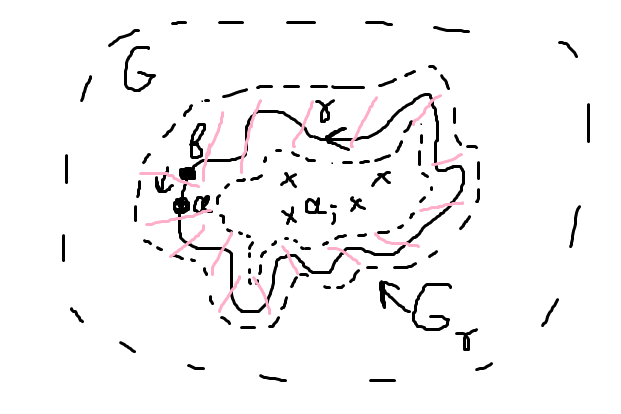
\includegraphics{Опр_логарифма.png}
		\caption{Картинка}
	\end{figure}
	С одной стороны получаем:
	$$\int\limits_{\gamma_{a,b}}\frac{f^{'}(w)}{f(w)}dw=\log f(b)-\log f(a)\underset{b\rightarrow a}{\longrightarrow}i\cdot\vartriangle_{arg}f(\gamma)$$
	С другой:
	$$\left|\oint\limits_{\gamma}\frac{f^{'}(w)}{f(w)}dw-\int\limits_{\gamma_{a,b}}\frac{f^{'}(w)}{f(w)}dw\right|\leq|b-a|\cdot M\underset{b\rightarrow a}{\longrightarrow}0,$$
	где $M$ максимум подынтыгральной функции на $\gamma$.
	Таким образом можем заключить, что:
	$$2\pi i\cdot\sum_{j=1}^nRes_{a_j}\frac{f^{'}}{f}=\oint\limits_{\gamma}\frac{f^{'}(w)}{f(w)}dw=i\cdot\vartriangle_{arg}f(\gamma)$$
	Теперь посчитаем вычет в особенности $a_j$. Из того что функция мероморфна имеет место следующее представление функции в виде ряда Лорана в малой окрестности особенности:
	$$f(z)=\sum_{n\geq k}c_n(z-a_j)^n$$
	$$f^{'}(z)=\sum_{n\geq k}n c_n(z-a_j)^{n-1}$$
	Тогда получаем следующее представление подынтегральной функции в окрестности каждой особенности:
	$$\frac{f{'}(z)}{f(z)}=\frac{k c_k(z-a_j)^{k-1}+(z-a_j)^k\varphi_1(z)}{c_k(z-a_j)^k+(z-a_j)^{k+1}\varphi_2(z)}=\frac{k}{(z-a_j)(1+(z-a_j)\psi (z))}+\chi (z)=$$
	$$=\frac{k}{z-a_j}+\frac{-k\psi (z)}{1_(z-a_j)\psi (z)}+\chi (z),$$
	где все неявно названные функции являются аналитичными в малой окрестности особенности.
	
	Таким образом интеграл равен $2\pi i\cdot k$, где $k$ - вычет и является порядком полюса или нуля функции $f$ и имеет знак, соответствующий особенности. Тем самым получена следующая теорема:
	\begin{theorem}\label{пр_арг}
		(Принцип аргумента) Пусть $f$ мероморфная функция в некоторой области $G$ и $\gamma$ некоторый контур в этой области. Тогда изменение аргумента $f$ при обходе контура равняется разности числа нулей и числа полюсов в области ограниченной контуром:
		$$\vartriangle_{arg}f(\gamma)=2\pi\cdot(N_0(f)-N_{\infty}(f))$$
	\end{theorem}
	\begin{consequence}
		У полинома степени $n$ в достаточно большом круге ровно $n$ нулей, так как из-за доминирующего члена граница намотается $n$ раз на больший круг.
	\end{consequence}
	\begin{theorem}\label{т_Руше}
		(Руше) Пусть $G$ односвязная область, $f,g$ аналитичны в некоторой области, содержащей окрестность $G$, $|f(z)|>|g(z)| \quad\forall z\in \partial G$. Тогда $f$ и $f+g$ имеют одинаковое число нулей в $G$.
	\end{theorem}
	\begin{proof}
		 По принципу аргумента\eqref{пр_арг} имеем следующие выражения для числа нулей функций:
		 $$N_f=\displaystyle\frac{1}{2\pi i}\oint\limits_{\partial G}\frac{f^{'}(z)}{f(z)}dz$$
		 $$N_{f+g}=\displaystyle\frac{1}{2\pi i}\oint\limits_{\partial G}\frac{f^{'}(z)+g^{'}(z)}{f(z)+g(z)}dz$$
		 Откуда получаем:
		 $$N_f-N_{f+g}=\displaystyle\frac{-1}{2\pi i}\oint\limits_{\partial G}\frac{\left(1+\frac{g(z)}{f(z)}\right)^{'}}{1+\frac{g(z)}{f(z)}}dz$$
		 Так как $|f(z)|>|g(z)| \quad\forall z\in \partial G$, то образ $\partial G$ - контур внутри шара $B_1(1)$ и тогда индекс 0 относительно образа границы нуль и значит наша разность интегралов равна нулю.
	\end{proof}
	Теорема используется для подсчета числа нулей сложных функций внутри каких-то областей, когда мы выделяем в функции доминирующий член на границе. Например \\$z^3+\frac{\sin z}{10}-\frac{1}{3}$ внутри $|z|<1$ имеет три корня.
	\section{Вычет в бесконечности}
	Рассмотрим функцию $f$, аналитичную во внешности круга $|z|>R$, что равносильно аналитичности в окрестности $\infty$. Поймем, что есть такое $f(\infty)$. Рассмотрим $g(z)=f(\frac{1}{z})$. Это аналитическая функция в окрестности нуля с особенностью в нем. Эту особенность мы умеем классифицировать по ряду Лорана $g(z)$ в 0 и соответственно таким образом классифицируем особенность $f(\infty)$. Теперь рассмотрим интеграл по контуру \\$\gamma :|z|=r>R$.
	$$\displaystyle\frac{1}{2\pi i}\oint\limits_{\gamma}f(z)dz=c_{-1}=Res_0f$$
	$$f(z)=\displaystyle\sum_{n=-\infty}^{+\infty}c_n z^n$$
	Теперь нам ничего не мешает увеличивать радиус контура, сдвигая его по сфере Римана к $\infty$, а там мы уже как бы получаем, что считаем таким образом $Res_{\infty}f$. Можно понять чему он равен, сделая следующую замену:
	$$f(z)dz=\displaystyle\left\{w=\frac{1}{z}\right\}=\frac{-1}{w^2}f\left(\frac{1}{w}\right)$$
	Тогда интеграл будет равен $-c_{-1}$.
	\begin{theorem}
		Пусть $f$ аналитична в $\widehat{\Co}\setminus\{a_1,\cdots,a_n\}$. Тогда $\displaystyle\sum_{k=1}^nRes_{a_k}f=0$.
	\end{theorem}
	\begin{proof}
		Если среди особых точек нет бесконечности, то тогда можно взять большой контур, внутри которого все особые точки, и тогда интеграл по нему это сумма вычетов, а с другой стороны, стягивая этот контур по сфере Римана к бесконечности, получаем, что интеграл равен вычету в бесконечности, то есть 0. Если бесконечность являлась особой точкой, то тогда интеграл по контуру равен сумме вычетов в точках, не являющихся бесконечностью, также он равен $c_{-1}$ из разложения $f$ в ряд Лорана в 0 и также он равен вычету в бесконечности, когда мы контур к ней стянем. Зная чему равен вычет в бесконечности из предыдущего рассуждения, получаем, что сумма 0.
	\end{proof}
	\section{Шварц и автоморфизмы единичного круга}
	Лирическое отступление. Хотим и можем сказать, что образ малой области есть малая область. Пусть функция $f$ имеет в точке $a$ ненулевую производную. Тогда имеем право написать $f(z)-f(a)=f^{'}(a)(z-a)+g(z)$, где $g(z)=o(|z-a|)$. Тогда в малой окрестности точки $a$ в правой части, доминирующий член будет $f^{'}(a)(z-a)$, откуда образ этой малой окрестности есть малая окрестность точки $f(a)$.
	\begin{definition}
		Функция $f$ называется однолистной в $G$, если она аналитична и инъективна в $G$.
	\end{definition}
	У однолистной функции автоматически есть голоморфная обратная функция, так как:
	\begin{proposition}
		Если $f$ однолистна, то $f^{'}(z)\neq 0$ в $G$.
	\end{proposition}
	\begin{proof}
		Смотреть доказательство теоремы о локальной однолистности в следующей лекции.
	\end{proof}
	Теперь поговорим об отображениях из $\{z: |z|<1\}=D$ в $D$, а именно классифицируем все автоморфизмы единичного круга. Самыми естественными примерами являются поворот и преобразование Мебиуса: $\Phi_a(z)=\displaystyle\frac{z-a}{1-\overline{a}z},\,\,|a|<1$. Оказыватся, что все наши автоморфизмы это комбинация этих двух. Чтобы получить это утверждение докажем полезную лемму.
	\begin{lemma}\label{л_Шварца}
		(Шварца) Пусть $f$ аналитична в $D$ и действует на нем в $D$, то есть $|f(z)|\leq 1$, а также $f(0)=0$. Тогда $|f(z)|\leq |z|$. Если еще для какой-то точки из круга окажется, что $|f(z_0)|=|z_0|$, то тогда $f(z)=e^{i\varphi}z$.
	\end{lemma}
	\begin{proof}
		Так как функция аналитична в круге, то мы можем написать ее ряд в 0, который будет иметь радиус сходимости 1, а также свободный коэффициент этого ряда будет равен 0. Таким образом мы имеем право поделить функцию на $z$. Радиус сходимости не уменьшится, так как в любом замкнутой подобласти круга, не содержащей 0, мы таким действием просто домножаем функцию на константу и аналитичность соответственно не теряется, а в 0 ряд сходится к функции, значит и в 0 функция аналитична.
		
		Можно было доказать аналитичность и по другому, а именно определить функцию $g(z)=\frac{f(z)}{z}$ для $z\neq 0$, в 0 положить $g(0)=f^{'}(0)$. Значение в нуле корректно из непрерывности, а функция будет голоморфна в круге, так как у нее есть явное выражение для производной вне 0, а по ее непрерывности можно получить, что $g^{'}(0)=\frac{f^{'}(0)}{2}$.
		
		Итак, мы получили, что $\frac{f(z)}{z}$ аналитична в круге, тогда по принципу максимума ее модуль внутри любого круга радиуса $r$ с центром в 0 не превосходит максимального значения на границе этого круга, которое не превосходит $r^{-1}$ из $|f(z)|\leq 1$. Тогда для произвольной точки $z_0\in D$ и для произвольного числа $|z_0|\leq r<1$ получаем неравенство $|f(z_0)|\leq |z_0|r^{-1}$, а тогда устремляя $r\rightarrow 1$ получаем $|f(z_0)|\leq |z_0|$.
		
		Пусть теперь для какой-то точки $|f(z_0)|=|z_0|$, то есть $|g(z_0)|=1$. Тогда из принципа максимума в окрестности этой точки $|g(z)|=1$ и тогда из теоремы о среднем получаем, что $g(z)\equiv const$.
	\end{proof}
	\begin{consequence}
		Пусть $f$ автоморфизм единичного круга и $f(0)=0$. Тогда $f(z)=e^{i\varphi}z$.
	\end{consequence}
	\begin{proof}
		Из того что это автоморфизм следует, что есть обратное отображение, причем оно тоже аналитично (однолистность вспоминаем) и в 0 принимает значение 0. Тогда для $f$ и обратного к нему можно применять лемму Шварца. Пусть нашлось такое $D\ni z_0\neq 0$, что $|z_0|\neq |f(z_0)|$. Тогда в зависимости от того, чей модуль больше, получаем противоречие с леммой Шварца для $f$ или обратного к нему. Значит модули равны и по лемме Шварца получаем требуемый вид $f$.
	\end{proof}
	Теперь наконец мы готовы доказать:
	\begin{theorem}
		Все аналитические автоморфизмы $D$ имеют вид $e^{i\varphi}\cdot\Phi_a(z)$.
	\end{theorem}
	\begin{proof}
		Пусть $f$ какой-то автоморфизм. Тогда $\Phi_{f(0)}(f(z))$ это автоморфизм, сохраняющий 0 и мы знаем его вид. Тогда решая линейное уравнение получаем:
		$$f(z)=e^{i\varphi}\displaystyle\cdot\frac{z-(-e^{-i\varphi}f(0))}{1-(-e^{i\varphi}\overline{f(0)})z}$$
	\end{proof}
	Теперь поговорим об отображениях комплексной плоскости в какие-то ее части аналитическими функциями, а точнее о том какие они бывают. Например мы не можем отобразить $\widehat{\Co}$ в $D$ потому что сфера не гомеоморфна диску. Также мы не можем отобразить $\Co$ в $D$, так как получим противоречие с теоремой Лиувилля. Но мы можем отобразить $\widehat{\Co}$ в себя отображениями вида $\displaystyle\frac{az+b}{cz+d}$, где $ad-bc\neq 0$ и только такими, а $\Co$ в себя только линейными. Доказательств видимо не будет $\rangle:<\quad \langle:($
	\section{Сходимость аналитичных функций, а также локальная однолистность}
	Рассмотрим множество $\mathcal{A}(G)$ всех аналитичных функций в области $G$.
	\begin{definition}
		Будем говорить, что $\{f_n\}_{n=1}^{+\infty}\subset\mathcal{A}(G)\quad f_n\rightarrow f$, если для любого компакта $K\subset G\quad f_n\rightrightarrows f$ на $K$. 
	\end{definition}
	\begin{proposition}
		Предельная функция из определения выше является аналитичной в области $G$.
	\end{proposition}
	\begin{proof}
		Во-первых, предельная функция является непрерывной в $G$, а тогда для аналитичности нам осталось показать:
		$$\oint\limits_{\gamma}f(z)dz=0\quad \forall\gamma\subset G$$
		Это делается нехитрой оценкой из равномерной сходимости и компактности контура:
		$$\left|\oint\limits_{\gamma}f(z)dz-\oint\limits_{\gamma}f_n(z)dz\right|\leq \oint\limits_{\gamma}|f(z)-f_n(z)|dz\leq \underset{z\in\gamma}{\max}|f(z)-f_n(z)|\cdot L(\gamma)\rightarrow 0$$
	\end{proof}
	\begin{proposition}
		За эквивалентное определение сходимости можно было принять равномерную интегральную сходимость на любом компакте(все функции аналитичны)
		$$\underset{n\rightarrow\rightarrow +\infty}{\lim}\int\limits_K |f_n(z)-f(z)|d\lambda_2(z)=0$$
	\end{proposition}
	\begin{proof}
		Интегральная сходимость следует из обычной, так как мера компакта конечна. Посмотрим, что происходит в другую сторону. Зафиксируем компакт и возьмем его $\varepsilon$-окрестность, лежащую в области. Покроем исходный компакт шарами радиуса $\varepsilon$. Тогда по теореме о среднем получаем:
		$$|f_n(z)-f(z)|=\left|\frac{1}{\lambda_2(B_{\varepsilon})}\int\limits_{B_{\varepsilon}}f_n(z)-f(z)d\lambda_2(z)\right|\leq\frac{1}{\pi\varepsilon^2}\int\limits_{K_{\varepsilon}}|f_n(z)-f(z)|d\lambda_2(z)\rightarrow 0$$
	\end{proof}
	Теперь поговорим о свойствах $\mathcal{A}(G)$. Во-первых, множество $\mathcal{A}(G)$ замкнуто относительно введеной сходимости, а также из наличия сходимости получаем топологию на множестве функций - аналитичных в каких-то подобластях $\Co$. Во-вторых, $\mathcal{A}(G)$ есть векторное пространство над $\Co$. В-третьих, данное пространство метризуемое. Можем представить $G$ в виде возрастающей цепочки компактов $K_i$ на каждом из которых определить метрику $\rho_i(f,g):=\min(1,\underset{z\in K_i}{\max}|f(z)-g(z)|)$. Тогда метрикой на всем пространстве можно положить $\displaystyle\rho (f, g):=\sum_{i=1}^{+\infty}\frac{1}{2^i}\cdot\rho_i(f,g)$.
	\begin{theorem}
		Если $f_n\rightarrow f$ в $\mathcal{A}(G)$, то $f_n^{'}\rightarrow f^{'}$ в $\mathcal{A}(G)$.
	\end{theorem}
	\begin{proof}
		Возьмем $B\Subset G(\Leftrightarrow\overline{B}\subset G)$. Тогда найдется $\varepsilon >0: B\subset B_{\varepsilon}\Subset G$. Воспользуемся т. Коши\eqref{формула_Коши}, положив $\gamma_{\varepsilon}: |z-w|=\varepsilon$.
		$$|f^{'}(z)|=\left|\frac{1}{2\pi i}\oint\limits_{\gamma_{\varepsilon}}\frac{f(w)}{(w-z)^2}dw\right|\leq\frac{1}{\varepsilon}\cdot\underset{z\in\gamma_{\varepsilon}}{\max}|f(z)|$$
		$$\underset{z\in B}{\max}|f_n^{'}(z)-f^{'}(z)|=\underset{z\in B}{\max}|(f_n(z)-f(z))^{'}|\leq\underset{z\in B_{\varepsilon}}{\max}|f_n(z)-f(z)|\cdot\frac{1}{\varepsilon}\underset{\varepsilon\rightarrow 0+}{\longrightarrow}0$$
	\end{proof}
	\begin{consequence}
		Из сходимости функций следует сходимость производных любого порядка.
	\end{consequence}
	\begin{theorem}\label{однолистноть_предел}
		(Об однолистности) Сходящаяся поледовательность однолистных функций сходится либо к однолистной, либо к константе.
	\end{theorem}
	\begin{proof}
		Пример сходимости к константе можно взять следующий: в качестве области выступает $\Co\setminus\{0\}$, в качестве функций $f_n(z)=C+\displaystyle\frac{1}{nz}$. Нетрудно видеть, что предельная функция равна $C$.
		
		Предположим противное. Тогда $\exists z_1\neq z_2:f(z_1)=f(z_2)$ и функция нк константна. Для удобства вычтем из каждой функции в последовательности константу $f(z_1)$. Тогда имеет место следующие рассуждения:
		$$f(z)=(z-z_1)^{k_1}g_1(z),\quad g_1(z_1)\neq 0\Rightarrow g_1(z)\neq 0 |z-z_1|\leq\varepsilon$$
		$$|f(z)|=\varepsilon^{k_1}|g_1(z_1)|+o(\varepsilon^{k_1})>\frac{\varepsilon^{k_1}}{2}g_1(z_1)$$
		Такое $k_1$- порядок нуля $z_1$ существует, иначе функция будет констатной. Аналогично можно написать и для $z_2$. Таким образом образ малой окрестности точек отделим от 0. Зафиксируем $\varepsilon$ и окружности вокруг наших точек соответствующего радиуса. Эти две окружности являются компактом, а значит можем воспользоваться определением сходимости функций, а именно с какого-то момента $|f|>|f-f_n|$. Тогда по теореме Руше\eqref{т_Руше} число нулей $f$ и $f+f_n-f=f_n$ одинакого внутри каждого круга вокруг точек $z_1,z_2$. У $f$ их два в нашем компакте, а тогда получаем противоречие с однолистностью $f_n$.
	\end{proof}
	\begin{definition}
		Функция называется локально однолистной в некоторой области, если для любой точки из области существует ее окрестность из области, в которой функция однолистна.
	\end{definition}
	\begin{theorem}\label{лок_однолист}
		(Критерий локальной однолистности) Функция локально однолистна тогда и только тогда, когда ее производная не обращается в 0 в этой области.
	\end{theorem}
	\begin{proof}
		Сначало в простую сторону, налево. Сдвинем функцию на константу для удобства:
		$$z_0:\quad f(z)=f^{'}(z_0)(z-z_0)+g(z),\quad g(z)=o(|z-z_0|)$$
		Предположим противное: в любой окрестности $z_0$ найдутся $z_1\neq z_2: f(z_1)=f(z_2)$. Тогда:
		$$0=f(z_1)-f(z_2)=f^{'}(z_0)(z_1-z_2)+g(z_1)-g(z_2)$$
		$$|g(z_1)-g(z_2)|\leq\left|\int_{z_1}^{z_2}g^{'}(w)dw\right|\leq|z_1-z_2|\cdot\underset{z\in B_{\varepsilon}}{\max}|g^{'}(z)|$$
		$$|g^{'}(z)|=\frac{1}{2\pi}\left|\oint\limits_{\gamma_{\varepsilon}}\frac{g(w)}{(w-z)^2}dw\right|\leq\frac{1}{\varepsilon}\underset{|z-z_0|\leq\varepsilon}{\max}|g(z)|$$
		Тем самым получаем: $0=f^{'}(z_0)(z_1-z_2)$ - противоречие.
		
		Напрааавоо! Пусть не так, тогда $\exists z_0:f^{'}(z_0)=0\Rightarrow f(z)=f(z_0)+(z-z_0)^kg(z):g(z_0)\neq 0,k\geq 2$. В какой-то малой окрестности $z_0$ имеет место $|g(z)|\geq a>0$, а тогда из определение логарифма $\exists h(z):\,e^{h(z)}=g(z)$ в этой окрестности. Значит имеется следующее представление:
		$$f(z)=f(z_0)+[(z-z_0)w(z)]^k,\quad w(z)=e^{\frac{h(z)}{k}}$$
		Возьмем $\xi:|\xi|<<1$ и покажем, что для любого $S\in\sqrt[k]{\xi}$ найдется решение уравнения $(z-z_0)w(z)=S$, откуда следует противоречие с локальной однолистностью. Из того что в какой-то малой окрестности $z_0$ функция $g(z)$ отделима от нуля следует, что $w(z)$ там тоже отделима от нуля и значит можно написать, что $w(z)=w(z_0)+o(|1|), w(z_0)\neq 0$. Тогда при уменьшении окрестности $|w(z_0)(z-z_0)|>|o(|z-z_0|)-S|$ и значит по теореме Руше число нулей в какой-то еще меньшей окрестности $z_0$ у функций $w(z_0)(z-z_0)$ и $w(z_0)(z-z_0)-S$ совпадает и их количесво хотя бы один. Откуда получаем решение уравнения $(z-z_0)w(z)=S$. Заметим, что для применение т. Руше мы и требовали $|\xi|<<1$. Так как решений нам достаточно в количестве хотя бы два, то процесс подгонки окрестностей можно делать конечное число раз и корни найдутся.
	\end{proof}
	\section{Теорема Монтеля и Римана}
	\begin{definition}
		Множество аналитичных функций в области $G$ называется компактным, если любая последовательность функций из множества содержит сходящуюся подпоследовательность.
	\end{definition}
	\begin{definition}
		Множество аналитичных функций $\mathcal{X}$ в области $G$ называется равномерно ограниченным, если $\forall K\Subset G-\emph{компакта}\forall z\in K\exists C>0:\forall f\in\mathcal{X}\,\, |f(z)|\leq C$.
	\end{definition}
	\begin{definition}
		Множество аналитичных функций $\mathcal{X}$ в области $G$ называется равностепенно непрерывным на компакте $K\subset G$, если $\forall\varepsilon>0\,\,\exists\delta>0\,\,\forall f\in\mathcal{X}\,\,\forall z_1,z_2\in K:$\\$|z_1-z_2|<\delta\Rightarrow |(f(z_1)-f(z_2)|<\varepsilon$
	\end{definition}
	\begin{definition}
		Множество аналитичных функций $\mathcal{X}$ в области $G$ называется локально равностепенно непрерывным на компакте $K\subset G$, если\\ $\forall\varepsilon>0\,\,\forall z_1\in K\exists\delta>0\,\,\forall f\in\mathcal{X}\,\,\forall z_2\in K:|z_1-z_2|<\delta\Rightarrow |(f(z_1)-f(z_2)|<\varepsilon$
	\end{definition}
	\begin{lemma}
		Из равномерной ограниченности функции в области $G$ следует равномерная ограниченность ее производной в той же области.
	\end{lemma}
	\begin{proof}
		Возьмем произвольный компакт $K$ и его $\varepsilon$-окрестность в области $G$, тогда:
		$$|f^{'}(z)|=\frac{1}{2\pi}\left|\oint\limits_{\gamma_{\varepsilon}}\frac{f(w)}{(w-z)^2}dw\right|\leq\frac{1}{\varepsilon}\cdot C(K_{\varepsilon})$$
	\end{proof}
	\begin{lemma}
		Из равномерной ограниченности множества функций следует локальная равностепенная непрерывность.
	\end{lemma}
	\begin{proof}
		Возьмем какой-то путь $\gamma$ (на самом деле отрезок, так как мы за локальность боремся и просто работаем в шаре малого радиуса вокруг $z_1$), соеденяющий $z_1$ и $z_2$, тогда из предыдущей леммы:
		$$|f(z_1)-f(z_2)|=\left|\oint\limits_{\gamma}f^{'}(w)dw\right|\leq L(\gamma)\cdot\underset{z\in K}{\max}|f^{'}(z)|\underset{z_1\rightarrow z_2}{\longrightarrow}0$$
	\end{proof}
	\begin{theorem}\label{Монтель}
		(Монтеля) Множество аналитичных функций $\mathcal{X}$ в области $G$ является компактным тогда и только тогда, когда оно равномерно ограничено.
	\end{theorem}
	\begin{proof}
		Докажем налево. По предыдущей лемме имеем локальную равностепенную непрерывность. Возьмем счетное всюдо плотное множество $\{z_i\}_{i=1}^{+\infty}\subset\Co$. Зафиксируем компакт $K$ и возьмем произвольную последовательность функций $\{f_n\}_{n=1}^{+\infty}$ из $\mathcal{X}$, а также оставим для работы только те числа из всюду плотного множества, которые попали в наш компакт. Для $z_1$ последовательность $\{f_n(z_1)\}_{n=1}^{+\infty}$ ограничена, а значит имеет сходящуюся подпоследовательность. Выберем какую-то сходящуюся подпоследовательность и дальше будем работать с ней. Берем $z_2$ и опять ограниченность и сходящаяся подпоследовательность. Таким образом получаем:
		$$\emph{сходятся при подстановке}\,\,z_1:f_{11},f_{12},f_{13}\cdots$$
		$$\emph{сходятся при подстановке}\,\,z_1,z_2:f_{21},f_{22},f_{23}\cdots$$
		$$\emph{сходятся при подстановке}\,\,z_1,z_2,z_3:f_{31},f_{32},f_{33}\cdots$$
		Выберем диагональные функции. Тогда получим последовательность функций $\{f_m\}_{m=1}^{+\infty}$ сходящуюся при подстановке $\{z_i\}_{i=1}^{+\infty}$. Теперь мы хотим проверить равномерную фундаментальность $\{f_m\}_{m=1}^{+\infty}$ в $K$.
		$$|f_n(z)-f_k(z)|\leq |f_n(z)-f_n(z_l)|+|f_k(z_l)-f_k(z)|+|f_n(z_l)-f_k(z_l)|<3\varepsilon,$$
		так как первые два модуля малы из локальной равностепенной непрерывности ($|z-z_l|<\delta$ из всюду плостности), а последний из сходимости $\{f_m\}_{m=1}^{+\infty}$ в точке $z_l$.
		
		Направо. Пусть не так, тогда есть компакт $K$ на котором можно выбрать последовательность функций и точек чтобы выполнялось $|f_n(z_n)|>n$. Тогда можно выбрать сходящуюся подпоследовательность точек и тогда в ней у функций полюс, а они аналитичны - противоречие.
	\end{proof}
	\begin{consequence}
		Пусть $\mathcal{X}$ множество аналитичных функций в области $G$, тогда следующие свойства $\mathcal{X}$ эквивалентны:
		\begin{enumerate}
			\item $\mathcal{X}$ компактно;
			\item $\mathcal{X}$ равномерно ограничено;
			\item $\mathcal{X}$ равностепенно непрерывно.
		\end{enumerate}
	\end{consequence}
	\begin{theorem}
		(Римана) Пусть $G$ односвязная область в $\widehat{\Co}$, которая имеет на своей границе хотя бы две точки. Тогда существует сюръективное однолистное отображение области на единичный круг.
	\end{theorem}
	\begin{proof}
		Определим класс функций $\mathcal{L}$ обладающих следующими свойствами:
		\begin{enumerate}
			\item $f\in\mathcal{L}\Leftrightarrow f\in\mathcal{A}(G)$;
			\item $f\in\mathcal{L}\Leftrightarrow f$ - однолистна или константна;
			\item $f\in\mathcal{L}\Leftrightarrow f(G)\subset G$.
		\end{enumerate}
		Зафиксируем какую-то точку $a\in G$ и определим функционал $J(f):=|f^{'}(a)|$. Мы хотим решить вариационную задачу - найти максимум этого функционала для дальнейшего доказательства теоремы. Заметим несколько простых свойств $\mathcal{L}$. Во-первых, оно замкнуто из теоремы\eqref{однолистноть_предел}, во-вторых, оно компактно из теоремы\eqref{Монтель}. Ранее мы показывали, что $\mathcal{A}(G)$ метризуемо, откуда следует непрерывность функционала, но также это можно понять из представления производной в точке через формулу Коши. Таким образом можно заключить, что максимум функционала реализуется на некоторой функции. Теперь давайте предьявим какую-то однолистную функцию в $\mathcal{L}$ откуда последует, что максимум не 0. Для этого всмпомним загадочное условие на принадлежность хотя бы двух точек границе.
		
		Итак, пусть $\alpha,\beta\in \partial G$. Тогда из односвязности определена функция $\varphi(z):=\displaystyle\sqrt{\frac{z-\alpha}{z-\beta}}$. Так как это корень, то есть две ветви $h_1,h_2$. Во-первых, каждая является однолистной функцией:
		$h(z_1)=h(z_2)\Rightarrow \frac{z_1-\alpha}{z_1-\beta}=\frac{z_2-\alpha}{z_2-\beta}\Rightarrow z_1=z_2$.
		Также понятно, что $h_1=-h_2$, откуда получаем пустоту пересечения образов $G$ этих функции:
		$$h_1(z_1)=h_2(z_2)\Rightarrow h_1(z_1)=-h_1(z_2)\Rightarrow z_1=z_2$$
		$$h_1(z_1)=h_2(z_1)\quad\emph{и}\quad h_1(z_1)=-h_2(z_1)\Rightarrow h_1(z_1)=0 - \emph{противоречие}$$
		Тогда возьмем $z_1\in h_1(G)$ и под искомое отображение подойдет $\varphi(z):=\displaystyle\frac{\varepsilon}{h_2(z)-z_1},\,\,\varepsilon<<1$.
		
		Пусть $\varphi_0(z)$ реализует максимум $J$ ($\varphi_0^{'}(a)\neq 0$). Пусть $\varphi_0(a)\neq 0$, тогда определим отображение $\psi_1:=\Phi_{\varphi_0(a)}\circ\varphi_0$.
		$$|\psi_1^{'}(a)|=\left|\frac{\varphi_0^{'}(a)}{1-|\varphi_0(a)|^2}\right|<1$$
		Тогда получаем, что $\varphi_0(z)$ не максимум функционала. Тогда $\varphi_0(a)=0$. Пусть $\varphi_0(G)\neq D$, тогда найдется точка $b\in D\setminus \varphi_0(G)$. Рассмотрим отображение $\displaystyle\psi_2:=\sqrt{\Phi_{b}\circ\varphi_0}$. Нетрудно видеть, что оно лежит в $\mathcal{L}$. Теперь посмотрим на отображение $\displaystyle h:=\Phi_{\psi_2(a)}\circ\psi_2$.
		$$|h^{'}(a)|=\left|\varphi_0^{'}(a)\cdot\frac{1+|b|}{2\sqrt{-b}}\right|>|\varphi_0(a)|$$
		Снова простиворечие с максимумом $J$, а значит $\varphi_0$ искомое отображение.
	\end{proof}
	\section{Принципы симметризации Рамана-Шварца}
	Список новых обозначений: $$\mathbb{T}=\partial\overline{D}, \Co^{+}=\{z:Im\,z>0\}, \Pi_r=\{z:0<Im\,z<r\}$$\par
	Важное лирическое оступление! Немного о продолжении аналитической функции. Во-первых заметим, что теорема Римана это просто теорема существования - функция есть и это все что мы знаем. Также есть такая теорема Каратеодори: условия как в теореме Римана, но граница области - жорданова кривая, тогда отображение продолжается до гомеоморфизма из $\overline{G}$ в $\overline{D}$. Также доказательство работает не только для областей на сфере Римана, а для любых римановых поверхностей. Дальше мы наверное будем заниматься аналитическими продолжениями, поэтому было сказано следующее. Пусть $G$ лежит в верхней полуплоскости и ее граница содержит отрезок $I$ на $\R$. Пусть есть аналитичная функция в $G$ и она непрерывно продолжается на $G\cup I$, при этом $f(I)\subset\R$, тогда она аналитично продолжается на $G\cup I\cup G_1$, где $G_1$ это сопряженное к $G$. Делается это так: в $G_1$ аналитична $h(z)=\overline{f(\overline{z})}$ и тогда можно склеить по $I$ функции $h$ и $f$. Непрерывность полученного отображения есть, осталось для аналитичности показать, что интеграл по границе любого прямоугольника в области 0. Интересен только случай, когда прямоугольник пересекает вещественную прямую, но тогда можно разбить область интегрирования на три прямоугольника, которые склены по центральному - узкому прямоугольнику вдоль вещественной оси и нужно проверить, что при уменьшении к нулю его ширины интеграл по нему стремится к нулю. Это так, так как модуль интеграла по вертикальным частям стремится к нулю, а по горизонтальным частям функции равномерно сходятся, но из-за интегрирования в противоположные стороны интегралы друг друга гасят.
	
	Еще немного примеров аналитических продолжений. Пусть $G$ - область аналитичности, $I$ - участок границы области. Сразу скажем, что проверка аналитичности везде одинаковая, как в примере выше, так что об этом тут писать не будем. Вообще есть два важных случай на тему аналитического продолжения на симметричную область относительно границы. Выше мы рассмотрели пример, когда функция была непрерывна на участке границы области аналитичности, который являлся отрезком вещественной прямой. Другой пример получается, когда функция непрерывна на границе, являющайся дугой $\mathbb{T}$, а образ дуги есть подмножество в $\R$. В этом случае на области, являющайся инверсной относительно $G$, аналитична функция $\displaystyle\overline{f\left(\frac{1}{\overline{z}}\right)}$. Другие два примера из этого сюжета: $I\subset\R,\,f(I)\subset\mathbb{T}$ и $I\subset\mathbb{T},\,f(I)\subset\mathbb{T}$. Отображения с которыми мы склеиваем исходные соответсвенно равны $\displaystyle\frac{1}{\overline{f(\overline{z})}},\,\frac{1}{\overline{f\left(\displaystyle\frac{1}{\overline{z}}\right)}}$.
	Тем самым доказали следующее:
	\begin{proposition}
		Пусть функция $f$ аналитична в области $G$ и непрерывна на $G\cup I$, где $I\subset\partial G$. Тогда $f$ аналитически продолжима на область $G\cup I\cup G_1$, где $G_1$ является следующей, в следующих случаях:
		\begin{enumerate}
			\item $I\subset\R,\,f(I)\subset\R,\,G_1=\{z:\overline{z}\in G\}$;
			\item $I\subset\R,\,f(I)\subset\mathbb{T},\,G_1=\{z:\overline{z}\in G\}$;
			\item $I\subset\mathbb{T},\,f(I)\subset\R,\,G_1=\{z:\frac{1}{\overline{z}}\in G\}$;
			\item $I\subset\mathbb{T},\,f(I)\subset\mathbb{T},\,G_1=\{z:\frac{1}{\overline{z}}\in G\}$.
		\end{enumerate}
	\end{proposition}
	\section{Базовые конформно-инвариантные отображения}
	\begin{proposition}\label{т_Каратеодори_слабая}
		Пусть $G$ - односвязная область с кусочно гладкой границей и $f$ функция со следующими свойствами: $f\in\mathcal{A}(G),\,f\in C(\overline{G}),\,f(\partial G)=\mathbb{T},\,Ind_{f(\partial G)}0=1$ (наматывается на окружность один раз). Тогда $f$ конформно инвариантное отображение $G$ на $D$, продолжаемое до гомеоморфизма замыканий областей.
	\end{proposition}
	Замечание: вместо круга можно рассматривать область с кусочно гладкой границей.
	\begin{proof}
		Единственное, что нам нужно показать, это что функция однолистна. Рассмотрим произвольную точку $w\in D$, тогда можем взять $\varepsilon>0$ и рассмотреть контур на расстоянии $\varepsilon$ от границы $G$ внутрь (эквидистантна) (тут мы используем, что граница кусочна линейна, так как эквидистантна будет такой же), такой что его образ будет близок к $\mathbb{T}$ и иметь индекс относительно $w$ равный одному. Тогда из принципа аргумента для функции $f(z)-w$ получаем, что у нее только один корень внутри области, ограниченной эквидистантной. Если для какого-то $w\in D$ существует больше одного прообраза, то тогда можно взять нужную эквидистантну и получится противоречие с принципом аргумента. Тем самым однолистность доказана, а продолжимость до гомеоморфизма следует из существования обратной функции и непррерывности $f$ и обратной на замыкании области.
	\end{proof}
	Классифицируем автоморфизмы $\Co^{+}$. Во-первых, понятно, что они имеют дробно-линей-ный вид $\displaystyle\frac{az+b}{cz+d}$, так как сначала можно перевести полуплоскость в круг отображением такого вида (инверсия+растяжение+сдвиг), затем применить автоморфизм круга, который тоже такого вида, а затем обратно в полуплоскость и снова тот же вид. Во-вторых, граница переходит в границу, а тогда подставляя точки $z=0, z=\infty$ получаем, что $\frac{b}{d},\frac{a}{c}\in\R$, а также прообраз произвольного вещественного числа есть (п.н.) вещественное число, а тогда получаем, что все коэффициенты должны быть вещественными. В-третьих, мы хотим однолистность, а тогда матрица отображения невырождена, т.е. $ad-bc\neq0$. В-четвертых, подставляя $z=i$ мы должны попасть в верхнюю полуплоскость, а значит мнимая часть при этой подстановки должна быть положительной, откуда получаем $ad-bc>0$. Суммируя результаты заключаем, что $a,b,c,d\in\R,\,ad-bc>0$. Также можно смотреть на эти автоморфизмы с другой стороны, а именно задавать их через отображение трех различных точек в три различные (три, потому что можно вообще считать детерминант равным 1). Для этого научимся переводить три любые различные точки в $0,1,\infty$, точнее посмотрим на обратное отображение, зная которое, знаем все что нужно.
	$$0\mapsto\frac{b}{d},\quad 1\mapsto\frac{a+b}{c+d},\quad \infty\mapsto\frac{a}{c}$$
	Теперь посмотрим на некоторые конформно инвариантные отображения.
	\begin{enumerate}
		\item Мы умеем дробно-линейными отображениями переводить полуплоскости в круги.
		\item Если взять $0<\alpha\in\R$, то отображение $z^{\alpha}$ переводит угол с раствором равным $\gamma$ в угол с раствором равным $\alpha\gamma$: а именно\\ $\{z:|z|\geq0, arg\,z\in(\frac{-\gamma}{2},\frac{\gamma}{2})\}\mapsto\{z:|z|\geq0, arg\,z\in(\frac{-\alpha\gamma}{2},\frac{\alpha\gamma}{2})\}$.
		\item Также одна из хороших функций это экспонента. Нетрудно видеть, представив коплексное число в виде $z=x+iy$, что она переводит открытую полосу $\Pi_{2\pi}$ в $\Co\setminus[0,+\infty)$, полосу $\Pi_{\pi}$ в $\Co^{+}$.
		\item Обратная функция к экспоненте $\log z:re^{i\varphi}\mapsto\log r+i\varphi$. Тем самым\\ $\Co\setminus(-\infty,0]\mapsto\{z:Im\,z\in(-\pi,\pi)\}$, то есть, внезапно, действительно обратная функция к экспоненте.
		\item Из предыдущих двух пунктов можем сказать между какими областями конфорно инвариантно отображение $z\mapsto z^{z_0}$, где $z_0\in\Co$. А именно $z\mapsto z^{z_0}=w,\,\log w=z_0\log z$. Область $\log z$ мы знаем, а домножение на $z_0$, это расширение полосы и ее поворот на некоторый угол. Дальше, чтобы получить $z^{z_0}$ надо взять экспоненту, а мы знаем что и куда она конформно переводит, то есть надо пересечь нашу расширенную повернутую полосу логарифма с полосой $\Pi_{2\pi}$ и посмотреть из чего это получается логарифмом. Вообще это Юрий Сергеевич оставил на подумать тому кто хочет, так что можно это не читать. Я вот подумал и придумал это, но не считаю себя умным, поэтому может тут и неправда или не вся правда.
		\item "Представьте, что вы открыли рот и закрыли. Конечно изначально речь шла не про рот, но...". Преобразование Жуковского: $w=\frac{1}{2}(z+\frac{1}{z})$ - переводит $\widehat{\Co}\setminus\overline{D}\mapsto\widehat{\Co}\setminus[-1,1]$, а вообще окружности с центром в нуле переходят в эллипсы с фокусами в -1, 1. Это можно понять, представив $z=re^{i\varphi},\,w=a+ib$. Вообще, если мы хотим понять, что данное преобразования однолистно в какой-то области, то просто из равенства образов каких-то точек $z_1,z_2$ получаем, что должно выполняться $z_1z_2\neq1$, то есть наши области - внешности круга и отрезка действительно подходят. Интересен случай обратного отображения к данному: $z=w\pm\sqrt{w^2-1}$. Разберемся с тем, почему оно аналитично в $\widehat{\Co}\setminus[-1,1]$. Для корня нам по-хорошему нужно выбирать ветвь, на которой он будет однозначен и обычно мы делаем разрез плоскости вдоль прямой, на которой подкоренное выражение вещественно и не превосходит 0. В нашем случае $\sqrt{w^2-1}=\sqrt{w-1}\sqrt{w+1}$, то есть сделаем два разреза вдоль лучей $(-\infty,-1],\,(-\infty,1]$. Вне этого функция без вопросов однолистна. Что происходит на $(-\infty,-1]$? Если бы у нас был просто $\sqrt{z}$, то у нас проблемы с однозначностью на отрицательной действительной оси, так как образ может оказаться либо на положительной мнимой оси, либо на отрицательной мнимой оси, то есть проблема со знаком числа. У нас же произведение двух корней и знаки одинаковы, тем самым они друг друга гасят и проблем с неоднозначностью не возникает.
	\end{enumerate}\par
	Теперь поговорим о конформно инвариантном отображении между колечками. \\$A=\{z:R_1<|z|<R_2\},\,B=\{z:R_1^{'}<|z|<R_2^{'}\}$. Если $\frac{R_2}{R_1}=\frac{R_2^{'}}{R_1^{'}}$, то понятное дело они конформно инвариантны. Что если отношения разные? Пусть есть конформно инвариантное отображение $f$. Для удобства считаем $R_1=1$. Из предыдущей лекции мы умеем аналитично продолжать $f$ на $\{z:\frac{1}{R_2}<|z|<R_2\}$ по принципу симметрии. Получим $f_1$, которое конформно инвариантно отображает $A$ в $B$, при этом функция аналитична в $\{z:\frac{1}{R_2}<|z|<R_2\}$. Далее снова продолжаем аналитично функцию к 0, получая счетную последовательность функций, предел которой есть функция $g$, которая конформно инвариантно отображает $A$ в $B$ и аналитична в $D\setminus\{0\}$ и действует в $D\setminus\{0\}$, то есть по лемме об устранимой особенности\eqref{лемма об устранимой особенности} наше отображение аналитично в единичном круге и заметим, что оно оставляет 0 на месте. Тогда по лемме Шварца\eqref{л_Шварца} $g$ есть поворот, а значит исходное отображение $f$ было поворотом и значит не могло быть конформно инвариантным отображением для колец с разным отношением радиусов.
	\section{Полуплоскость в прямоугольник}
	До этого мы рассматривали конформно инвариантные отображения бесконечных областей между собой, поэтому теперь научимся отображать круг в прямоугольник, а вообще данный метод обощается на отображения круга в многоугольник следующим важным соображением: полуплоскость это многоугольник с углами величиной $\pi$. Круг мы умеем перегонять в полуплоскость, поэтому построим отображение полуплоскости в прямоугольник, которое аналитично в открытой полуплоскости, непрерывно на границе - вещественной прямой и наматывает прямую один раз на границу прямоугольника. Если такое получится, то по \eqref{т_Каратеодори_слабая} получим, что данное отображение конформно инварантно.
	
	Итак, положим $\kappa\in(0,1)$ и определим:
	$$\varphi(z)=\int_0^z\frac{dt}{\sqrt{(1-t^2)(1-t^2\kappa^2)}}=\int_0^zf(t)dt$$
	Функция аналитична в верхней полуплоскости, так как корни там извлекаются и под интегралом аналитичная функция, а это также показывает непрерывность на вещественной прямой. Поймем, что образ вещественной будет границей какого-то прямоугольника. Будем интегрировать постепенно. $\varphi(0)=0,\varphi([0,1))\subset\R$, при этом $\varphi(1)=K<+\infty$. То есть не отрезке $[0,1]$ при интегрировании рост функции был чисто вещественным. Рассматривая $\displaystyle\int_1^xf(t)dt$, заметим, что под корнем отрицательное число, поэтому появляется множитель $i$ и рост $\varphi(z)$ чисто мнимый, $\varphi(\frac{1}{\kappa})=K+iL$. На участке $[\frac{1}{\kappa},+\infty)$ интеграл конечен и имеет отрицательный вещественный рост. То есть образ положительной вещественной оси есть прямоугольная рамка в верхней полуплоскости с началом в 0. Так как подынтегральная функция четная, то образ отрицательной оси такая же рамка, но с другой стороны относительно мнимой оси. Остается вопрос с тем, не накладываются ли они друг на друга и ответ нет, так как мы интегрируем петлю на сфере Римана.
	\begin{figure}[H]
		\centering
		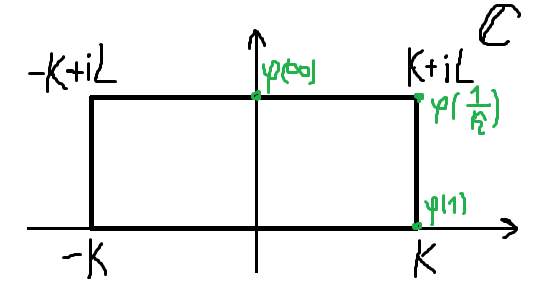
\includegraphics{конформное_плоскость_прям.png}
		\caption{Образ вещественной прямой}
	\end{figure}
	Теперь покажем, что меняя параметр $\kappa$ мы можем сделать произвольное соотношение сторон. Для этого заметим, что $K$ и $L$ меняются непрерывно по $\kappa$, так как подынтыгральная функция непрерывно зависит от $\kappa$, и при $\kappa\rightarrow0,\,L\rightarrow+\infty; K$ - ограничено, а при $\kappa\rightarrow1,\,K\rightarrow+\infty; L$ - ограничено.
	\section{Эллиптический синус}
	Посмотрим на обратное отображение $f$ к тому, которое мы построили в прошлый раз. Это конформно инвариантное отображение прямоугольника $P_1$ в верхнюю полуплоскость, причем у нас очень хороший прямоугольник (границы параллельны осям и одна из них вещественна) и образ его границы тоже хороший - вещественный. Тогда по принципу симметрии мы умеем аналитически продолжать функцию на больщую область, а именно на симметричный прямоугольник $P_2$ снизу. Также функция $g(z):=\overline{f(2K-\overline{z})}$ аналитична на $P_3$ и совпадает на $P_1\cap P_3$ с функцией $f$. То есть аналитично продлили на еще один прямоугольник. Теперь остался последний прямоугольник $P_4$ для завершения картины рассуждений, на который аналитично продлить функцию можно двумя способами: с $P_2$ и с $P_3$. Хотелось бы, чтобы оба продолжения совпали и это так:
	$$g(z)=\overline{f(2K-\overline{z})},\,h(z)=\overline{f(\overline{z})}\Rightarrow \overline{g(\overline{z})}=\overline{h(2K-\overline{z})}=w(z)$$
	\begin{figure}[H]
		\centering
		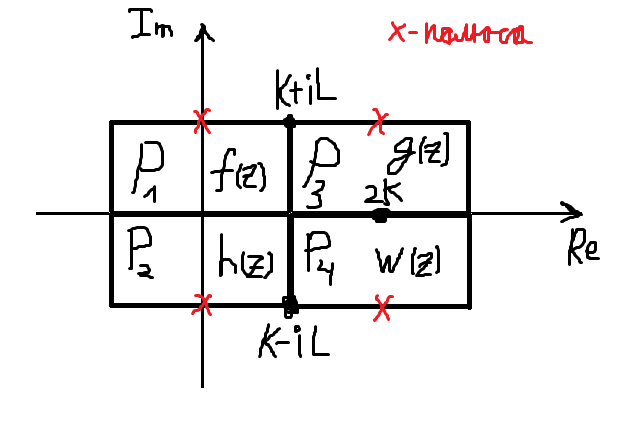
\includegraphics{function_sn.png}
		\caption{Продолжение на плоскость}
	\end{figure}
	Таким образом можем продолжить функцию на всю плоскость и получить двоякопериодическую функцию.
	\begin{equation*}
		\begin{cases}
			Sn(z+4K)=Sn(z)\\
			Sn(z+2iL)=Sn(z)
		\end{cases}
	\end{equation*}
	Вопрос-ловушка: функция определена во всей плоскости, а по факту на компакте и при этом не константная, как так? Кажется противоречие с т. Лиувилля, но это ложь ввиду мероморфности функции, так как $f(iL)=\infty$. Полученная функция называется эллиптическим синусом $Sn(z,\kappa)$, которая зависит от параметра $\kappa$.
	
	Теперь поймем что из себя представляет единственная особенность нашей функции (которая сидит на периодичной решетке $2K\mathbb{Z}\times(L+2L\mathbb{Z})$). Сразу заметим, что это полюс, ибо предел по любому направлению к ней есть бесконечность (по модулю). Далее посмотрим на малую проколотую окрестность точки $iL$. Та ее часть, что сидит в исходном прямоугольнике переходит во внешность некоторой окрестности 0 пересеченной с вехней полуплоскостью, а часть из верхнего прямоугольника перейдет во внешность некоторой окрестности 0 пересеченной с нижней полуплоскотью по построению $Sn$, а общая граница прямоугольников перейдет в вещественную прямую с вырезом некоторой окрестности 0. Заметим, что на частях из прямоугольников функция однолистна, а на границе она биективна, то есть в малой окрестности $iL$ функция однолистна. А однолистная функция не может иметь полюс порядка больше одного, так как в окрестности полюса она ведет себя как $C(z-z_0)^{-n}$ и при $n>1$ нарушалось бы условие однолистности.
	\section{Кристоффель-Шварц}
	Вот мы все поняли про конформно инвариантное отображение прямоугольника в полуплоскость (кроме явного вида формулы). Следующий вопрос, который частично затрагивался, а что можно сказать про другие многоугольники? Пусть мы хотим конформно инвариантно отобразить полуплоскость в многоугольник с углами $\{\alpha_k\}_{k=1}^n:0<\alpha_k<2\pi$. Во-первых, знаем формулу $\displaystyle\sum_{k=1}^n\alpha_k=\pi(n-2)$, а также то, что полуплоскость это многоугольник с углами в $\{a_k\}_{k=1}^n:0<a_1,\,a_i<a_{i+1}$ и его углы равны $\pi$, а должны стать равны $\alpha_k$. Из этого соображения получаем асимптотику в критических точках и нужную формулу Кристоффеля-Шварца:
	\begin{equation}
		\varphi(z)=\int_0^z\prod_{k=1}^n(t-a_k)^{\frac{\alpha_k}{\pi}-1}dt
	\end{equation}
	В показателях степени вычитается 1, так как при интегрировании она добавится. Теперь кратко скажем почему эта формула делает то что надо. С верхней полуплоскостью нет вопросов, перейдет во внутренность того что получится. Также $\displaystyle\sum_{k=1}^n\left(\frac{\alpha_k}{\pi}-1\right)=-2$, а значит в бесконечности интеграл сходится и $\infty\mapsto z\in\Co$. Почему при интегрировании участков между $a_i$ получать в образе будем отрезки можно понять, если  заметить, что переходе через очередную вершину из соответсвующего монома выносится множитель $e^{i\alpha_k}$ (расписать моном через комплексную экспоненту) и далее снова вещественный интеграл. То есть мы в вершине повернули вектор вдоль которого строим образ и дальше увеличиваем его длину.
	\begin{figure}[H]
		\centering
		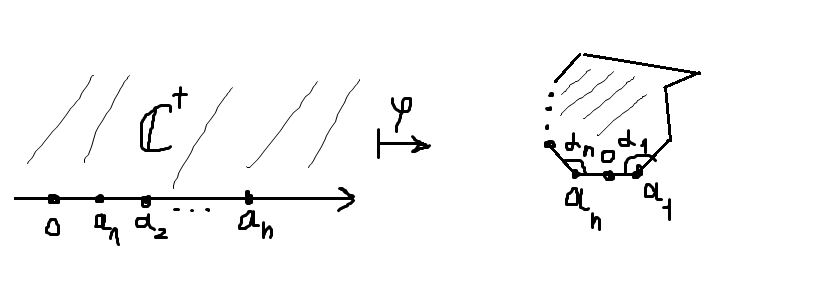
\includegraphics{Кристоффель_Шварц.png}
		\caption{Поясняющая картинка}
	\end{figure}
	Следующий вопрос а все ли многоугольники мы так получим? Он сложный и ответ на него не сказали, но сказали почему вопрос сложный. Заметим, что при таком подходе мы не контролируем длины сторон, а только углы многоугольника. С прямоугольником получилось, так как он задается отношениями сторон, которое мы могли произвольно менять. Нас может спасти то, что своими углами многоугольник задается однозначно, но это геометрический вопрос, так что долой.
	
	Заметим что таким подходом мы можем построить не только многоугольник но и вообще какую угодно кусочно линейную кракозябру, в плане что какие-то части могут уходить на бесконечность (просто на сфере Римана в бесконечности будут склеены вершины нужных углов). Например следующая формула строит штучку с картинки ниже (уходящие на бесконечность прямые могут пересечься и это нормально), если сумма углов достаточно большая.
	$$\varphi(z)=\int_0^z\prod_{k=1}^{n-1}(t-a_k)^{\frac{\alpha_k}{\pi}-1}dt$$
	$$\sum_{k=1}^{n-1}\alpha_k\geq\pi(n-2)\Rightarrow\sum_{k=1}^{n-1}\left(\frac{\alpha_k}{\pi}-1\right)\geq-1\Rightarrow\infty\mapsto\infty$$
	\begin{figure}[H]
		\centering
		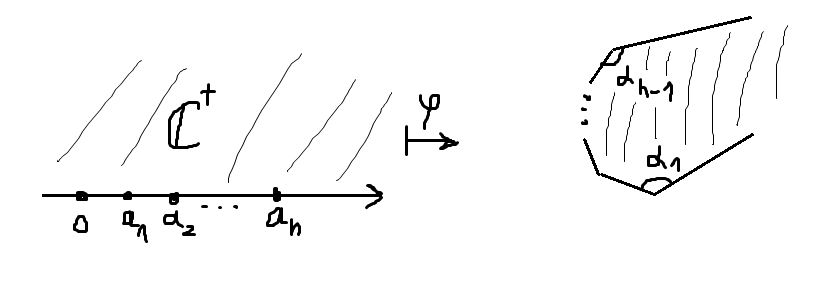
\includegraphics{Кристоффель_Шварц2.png}
		\caption{Поясняющая картинка}
	\end{figure}
	Ну и бонусом пример с переводом полуплоскости в полуполосу \\$\{z:Im\,z\geq0,\,\,Re\,z\in[\frac{-\pi}{2},\frac{\pi}{2}]\}$:
	$$\varphi(z)=\int_0^z\frac{dt}{\sqrt{1-t^2}}$$
	\section{Малая теорема Пикара}
	\begin{theorem}
		(Малая теорема Пикара для целых функций) Неконстантная целая функция принимает все значения в $\Co$, кроме быть может одного.
	\end{theorem}
	\begin{consequence}
		(Малая теорема Пикара для мероморфных функций) Мероморфная функция принимает все значения в $\overline{\Co}$, кроме быть может двух.
	\end{consequence}
	Заметим, что следствие очевидно, поэтому докажем теорему для целых.
	\begin{proof}
		Докажем от противного. Линейным преобразованием можем перевести плоскость в себя так, чтобы целая функция $f$ не принимала значения 0 и 1. По теореме Римана существует функция $\varphi$ конформно-инвариантно переводящая треугольник из трех дуг попарно перпендикулярных окружностей в верхнюю полуплоскость, а также можем добиться того, чтобы вершины переводились в точки $0,1,\infty$.
		\begin{figure}[H]
			\centering
			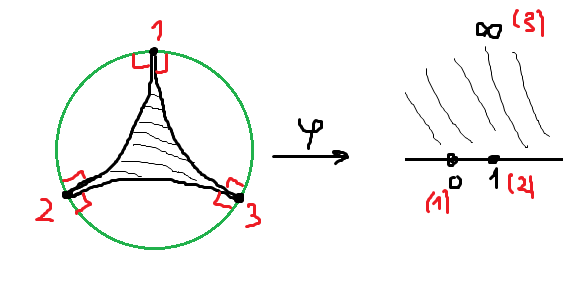
\includegraphics{Треугольник.png}
			\caption{Поясняющая картинка}
		\end{figure}
		Будем пользоваться принципом симметрии и продлим функцию до аналитичной $\mu$ из единичного диска, при этом продливать будем конформно-инвариантно, чтобы иметь возможность взять обратную функцию и соответсвенно получим в качестве образа некую риманову поверхность. Теперь если строго: будем действовать пошагово. На каждом шаге будем иметь конформно-инвариантное отображение из "звездного" множества в риманову поверхность - конечного дерева, где в качестве вершин будут замкнутые полуплоскости без двух точек на границе, склееные по общим отрезкам на границе. По принципу симметрии отразим звездное множество относительно каждой дуги, тем самым расширив область которую конформно-инвариантно отображаем, а при отражение через дугу с концами в точках, образы которых две из $0,1,\infty$, приклеим к соответствующей вершине римановой поверхности замкнутую полуплоскость без точек 0 и 1 на границы, по участку границы, являющимся образом дуги, относительно которой отражали.
		\begin{figure}[H]
			\centering
			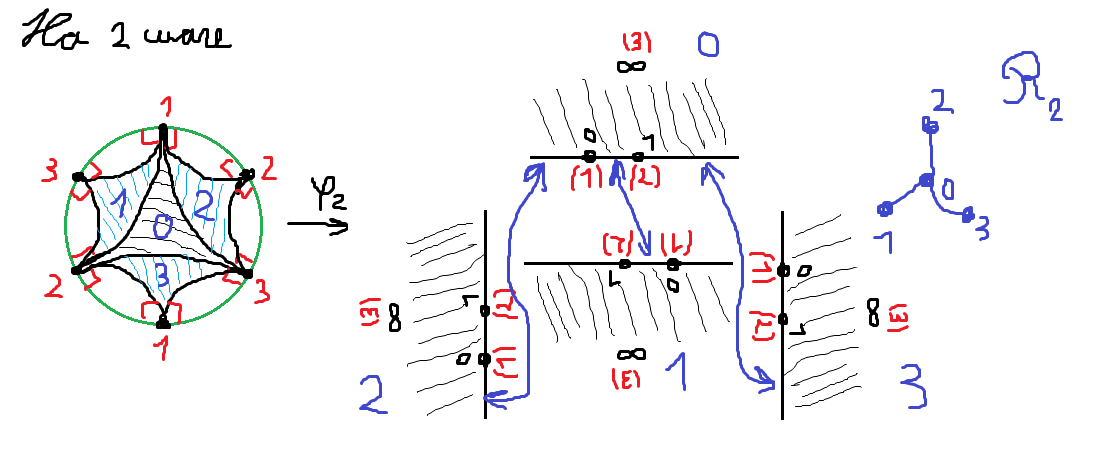
\includegraphics{Второй_шаг_Пикар.png}
			\caption{Поясняющая картинка}
		\end{figure}
		Продолжая процесс счетное число раз получим функцию $\mu$ конформно-инвариантно отображающую единичный диск в следующее бесконечное дерево:
		\begin{figure}[H]
			\centering
			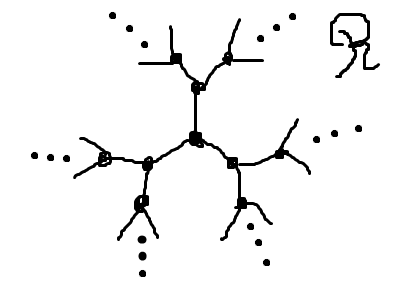
\includegraphics{Граф_Кели_Пикар.png}
			\caption{Поясняющая картинка}
		\end{figure}
		Почему отобразили весь диск? Потому что на каждом следующем шаге процесса появляются образы середин старых дуг единичной окружности, тем самым в пределе отображаем счетное плотное множества с единичной окружности, а так как дуги соеденяющие точки с границы диска все ближе к границе (можно формулку написать, можно картинку нарисовать), то для любой точки из диска найдется шаг процесса, который ее захватил.
		
		Теперь можем взять $\mu^{-1}$, которая будет действовать из $\mathfrak{R}$ в единичный диск и если мы сможем определить $\mu^{-1}(f(z))$, то получим целую функцию, действующую в диск, то есть по т. Лиувилля она будет константной, а это не так из предположения непостоянства функции $f(z)$. Покажем, что композиция определена. Можем считать, что $f(i)\in\Co^{+}$. Рассмотрим произвольную точку плоскости $z$ и возьмем произвольный путь $\gamma$ от $i$ до $z$. Посмотрим на $f(\gamma)$. Так как $f$ не принимает значения 0 и 1, то данный путь каждый раз, когда пересекает вещесвенную ось, пересекает ее по одному из трех интервалов, по которым мы склеивали полуплоскости, получая $\mathfrak{R}$. Тогда образ этого пути можно задать на $\mathfrak{R}$, а именно он совпадает на каждой вершине поверхности с соответствующим участком на исходной плоскости, а при переходе через интервал на вещественной оси переходит по соответсвующему ребру на другую вершину. Так как полученная поверхность односвязна (локально конечное дерево), то образы путей гомотопны, а значит $\mu^{-1}(f(z))$ определено однозначно.
	\end{proof}
	\section{Всегда ли можно аналитически продолжать функцию?}
	Мы что-то выучили про конформно-инвариантные отображения. Следующий логичный вопрос это аналитические продолжения. Ранее мы аналитично продолжали функцию через границу области, если она была хорошей и ее образ тоже. Можем ли мы всегда продолжить любую аналитичную функцию на большую область? Оказывается нет. Пусть задана аналитичная функция $f(z)$ на односвязной области $G$, граница которой содержит хотя бы две точки (чтобы имел смысл вопрос об аналитичном продолжении, а то почти целую функцию некуда продолжать). Теорема Римана говорит, что имеется конформно-инвариантное отображение $\varphi(z)$ этой области на единичный круг. Тем самым можем изучать продолжимость аналитичной функции, заданной на единичном круге.
	
	Можем сразу получить отрицательный ответ операцией рассмотрим функцию\\ $f(z)=\displaystyle\sum_{n=0}^{+\infty}z^{2^n}$. Понятно, что радиус сходимости в нуле хотя бы один. Посмотрим, почему нет аналитичного продолжения за единичный круг ни в каком месте. Возьмем произвольное $N\in\mathbb{N}$ и посмотрим на точки $z=re^{2\pi i\frac{k}{N}}$, где $k\in\mathbb{N}$. Как нетрудно видеть хвост ряда будет выглядеть так: $r^{2^N}+r^{2^{N+1}}+\cdots$. Тем самым при $r=1$ получаем, что хвост расходится, а ввиду произвольного выбора $k,N$ получаем, что ряд расходится по крайней мере на двоично-рациональных углах, тем самым для данной функции не может существовать даже мероморфного продолжения за любой участок единичного круга, так как тогда по теореме единственности\eqref{т_единственности} получили бы, что функция тождественно равна бесконечности. Замечание: Юрий Сергеевич назвал эту функцию функцией Блоха, но я не нашел достоверных подтверждений этому в интернете.
	
	Из этого примера можно получить общую идею конcтруирования аналитичных функций в круге, которые не имеют аналитичного продолжения. Из теоремы единственности\eqref{т_единственности} мы знаем, что в любом компакте конечное число нулей функции, но ничего не мешает скапливаться им на границе области. Значит если построим функцию с нулями $\{z_k\}$, такими что $\overline{\{z_k\}}\supset\mathbb{T}$, то у нее не будет аналитичного продолжения за круг. Добавлять нули к функции очень просто - надо просто домножить на соответсвующий моном, но есть проблема со сходимостью, когда произведение станет бесконечным, поэтому сначала изучим сходимость произведений Бляшке.
	\begin{definition}
		Пусть дана последовательность $\{z_k\}_{k=1}^T:\,z_k\in D,\,T\in(\mathbb{N}\cup\{+\infty\}),$ \\$\forall 0\leq r<1\,\,card(\{z_k\}_{k=1}^T\cap B_r(0))<+\infty$. Тогда соответствующим произведением Бляшке будем называть функцию:
		$$B_T(z)=\prod_{k=1}^T\left(\frac{|z_k|}{z_k}\cdot\frac{z_k-z}{1-\overline{z_k}z}\right)$$
	\end{definition}
	\begin{proposition}
		Произведение Бляшке сходится тогда и только тогда, когда \\$\displaystyle\sum_{k=1}^T(1-|z_k|)<+\infty$.
	\end{proposition}
	\begin{proof}
		При $T<+\infty$ очевидно. Слева направо: $B_T(0)<+\infty\Leftrightarrow\displaystyle\sum_{k=1}^T(1-|z_k|)<+\infty$. Докажем в обратную сторону. Фиксируем $z$, тогда:
		$$\frac{|z_k|}{z_k}\cdot\frac{z_k-z}{1-\overline{z_k}z}=|z_k|\frac{1-\frac{z}{z_k}}{1-\overline{z_k}z}=|z_k|\left(1+\frac{\overline{z_k}z-\frac{z}{z_k}}{1-\overline{z_k}z}\right)=1+(|z_k|-1)+\frac{|z_k|^3z-|z_k|z}{z_k(1-\overline{z_k}z)}=$$
		$$=1+(|z_k|-1)\left(1+\frac{z|z_k|(|z_k|+1)}{z_k(1-\overline{z_k}z)}\right)$$
		Нетрудно видеть, что:
		$$\left|1+\frac{z|z_k|(|z_k|+1)}{z_k(1-\overline{z_k}z)}\right|<C_z<+\infty$$
		Откуда получаем:
		$$|B_T(z)|<\prod_{k=1}^{+\infty}(1+(1-|z_k|)C_z)<+\infty\Leftrightarrow\sum_{k=1}^T(1-|z_k|)<+\infty,$$
		как нам известно из вещественного анализа, а критерий Вейерштрасса завершает доказательство.
	\end{proof}
	Возвращаясь к конструированию примера не продолжимой аналитичной функции положим для каждого $n\in\mathbb{N}$ набор комплексных чисел $z_{n,k}=(1-\frac{1}{2^n})e^{2\pi i\frac{k}{n}}$, где $k\in\overline{0,n-1}$ и построим по ним произведение Бляшке. Так как $\displaystyle\sum_{n,k}(1-|z_{n,k}|)=\sum_{n=1}^{+\infty}\frac{n}{2^n}<+\infty$, то функция аналитична в круге, а также ввиду выбора корней получаем $\overline{\{z_{n,k}\}}\supset\mathbb{T}$.
	
	Замечание: если произведение конечно, то $B_n(z)$ является n-листной функцией, так как для любого $w:|w|<1$ имеем n решений уравнения $B_n(z)=w$ по принципу аргумента. Аналогичное утверждение для бесконечного произведения сказать сложно и мы не будем говорить.
	\section{Формула Пуассона}
	Рассмотрим следующую задачу: как сконструировать аналитичную функцию в некоторой области? В данный момент у нас есть два тривиальных способа: записать ряд функции, записать бесконечное произведение Бляшке. Записать мы можем, но понять где функция будет аналитична и вообще что-то осмысленное про функцию будет сложно. Следующий вариант, это вспомнить формулу Коши\eqref{формула_Коши}, которая говорит нам, что если мы знаем функцию на границе круге, то мы знаем ее и внутри круга. Теперь сделаем следующий фокус: возьмем измеримую функцию $g(z)\in L^1(\mathbb{T})$ или вообще меру и определим
	$$f(z)=\frac{1}{2\pi i}\oint\limits_{\mathbb{T}}\frac{g(w)}{w-z}dw$$
	Получаем таким образом аналитичную функцию внутри круга. Теперь заметим, что вместо окружности можно брать любой другой гомотопный ей контур. Следующий логичный вопрос о том как связаны $f$ и $g$ кроме как равенством через интеграл довольно интересен, но видимо мы им сейчас заниматься не будем. Вместо этого заметим, что чем еще прекрасен комплексный анализ - знали аналитичную функцию на границе, значит восстановим и внутри. Но вот оказывается, что можно знать на границе не всю функцию, а только ее вещественную часть. Это кажется логичным, так как вещественная часть является гармонической функцией, а значит с точностью до константы ей соответствует единственная гармонически сопряженная, а гармоническую мы тоже можем восстановить по значениям с границы. Покажем это строго.
	
	Пусть $f(z)$ аналитична в круге радиуса $1+\varepsilon$ и $Im\,f(0)=0$ для удобства. Тогда имеем следующие представления:
	$$u(z)+iv(z)=f(z)=\sum_{n=0}^{+\infty}a_nz^n$$
	Зафиксируем произвольное $z=re^{i\theta}\in D$ и напишем простую выкладку:
	$$u(z)=Re\,(\sum_{n=0}^{+\infty}a_nz^n)=a_0+\frac{1}{2}\sum_{n=1}^{+\infty}(a_nz^n+\overline{a_n}\overline{z}^n)=a_0+\frac{1}{2}\sum_{n=1}^{+\infty}(a_nr^ne^{in\theta}+\overline{a_n}r^ne^{-in\theta})$$
	Теперь заметим следующее:
	$$u(e^{i\theta})=a_0+\frac{1}{2}\sum_{n=1}^{+\infty}(a_ne^{in\theta}+\overline{a_n}e^{-in\theta})$$
	$$a_0=\frac{1}{2\pi}\int_0^{2\pi}u(e^{i\theta})d\theta,\quad a_n=\frac{1}{\pi}\int_0^{2\pi}u(e^{i\theta})e^{-in\theta}d\theta$$
	Откуда получаем:
	$$u(z)=\frac{1}{2\pi}\int_0^{2\pi}u(e^{it})\left(1+\sum_{n=1}^{+\infty}r^ne^{in(\theta-t)}+\sum_{n=1}^{+\infty}r^ne^{-in(\theta-t)}\right)dt=$$
	$$=\frac{1}{2\pi}\int_0^{2\pi}u(e^{it})\left(\frac{1}{1-re^{i(\theta-t)}}+\frac{1}{1-re^{-i(\theta-t)}}\right)dt=$$
	$$=\frac{1}{2\pi}\int_0^{2\pi}u(e^{it})\frac{1-r^2}{1+r^2-2r\cos(\theta-t)}dt=\frac{1}{2\pi}\int_0^{2\pi}u(e^{it})Re\,\left(\frac{e^{it}+z}{e^{it}-z}\right)dt$$
	$$\emph{Ядро Пуассона}: P_r(\theta)=\frac{1-r^2}{1+r^2-2r\cos(\theta)}\quad\emph{ядро Шварца}: S_z=\frac{e^{it}+z}{e^{it}-z}$$
	Тем самым получаем, что ядро Пуассона решает задачу Дирихле для вещественной части, а написав аналогичную выкладку для всей комплексной функции получаем, что задачу Дирихле для нее решает ядро Шварца:
	$$u(re^{i\theta})=u(e^{it})*P_r(\theta)\quad f(z)=u(e^{it})*S_z$$
	\section{Восстановление функций с ограниченной $L^p$ нормой (из $H^p$)}
	Следующий материал частично посвящен пространствам Харди, без их явного упоминания, по факту мы здесь почти забыли комплексный анализ и занимаемся гармоническим анализом и теорией меры, чтобы решать задачу Дирихле, также здесь частично затрагивается функциональный анализ, который здесь не будет написан больше чем в формате определений и формулировок теорем, так как Юрий Сергеевич сказал, что в программу экзамена он входить не будет, поэтому я не имею желания расписывать и доказывать его подробно, а кому очень сильно надо могут ходить к профессору Пеллеру или все же нормально изучать функциональный анализ, а именно читая НОРМАЛЬНЫЕ книги (НЕ Конвея, а например Рудин, Берри Саймон, Сёкефальви-Надь, Богачев). Также, если вам кажется, что некоторые лекции подозрительно малы в объеме, то там просто доказывались какие-то факты из функана, либо люди задавали идиотские вопросы, на которые Юрий Сергеевич почему-то долго и подробно отвечал. Но не переживайте, я попросил, чтобы лекций было на две больше (а вообще хочу добится чтобы было 24 вместо 20), так что еще будет много интересного.
	
	В прошлый раз мы установили, что если от гармонической вещественнозначной функции в круге с запасом нам даны только ее значения на границе, то написав ее свертку с ядром Пуассона на границе мы восстановим функцию в круге. Оказывается и этого слишком много для того чтобы восстановить гармоническую функцию.
	
	Пусть нам дана гармоническая функция в единичном круге $u:\Co\rightarrow\R$, про которую нам ничего не известно на границе (то есть сразу предыдущим результатом мы воспользоваться не можем), но нам известно, что у нее ограничен рост нормы в $L^p$ по внутренним окружностям для какого-то фиксированного $p$:
	$$\sup\limits_{0<r<1}\frac{1}{2\pi}\int_0^{2\pi}|u(re^{it})|^pdt=\sup\limits_{0<r<1}||u||_{L^p(r\mathbb{T})}^p<+\infty$$
	Наша следующая цель установить, что для такой функции существует функция\\ $U\in L^p(\mathbb{T})$, по которой уже можно восстановить некую аналитичную функцию $f$ в круге, при этом $Re\,f=u$ внутри круга.
	
	Для начала разберем приятный случай Гильбертого пространства, а именно $p=2$.
	\begin{proposition}
		Пусть гармоническая функция $u:D\rightarrow\R$ имеет ограниченый рост нормы в $L^2$, а именно:
		$$\sup\limits_{0<r<1}||u||_{L^2(r\mathbb{T})}<+\infty,$$
		тогда существует функция $f\in L^2(\mathbb{T})$, такая что $u=\frac{1}{2\pi}f*P_r$
	\end{proposition}
	\begin{proof}
		Для произвольного $0<r<1$ положим $u_r(t)=u(re^{it})$ - периодические функции из отрезка $[0,2\pi]$. Из предыдущей лекции (когда восстанавливали вещественную часть функции по границе) имеем разложение $u_r(t)$ в так называемый ортонормированный ряд Фурье:
		$$u_r(t)=|a_0|+\frac{1}{2}\sum_{n=1}^{+\infty}(a_nr^ne^{int}+\overline{a_n}r^ne^{-int})$$
		Откуда получаем, что $L^2$ норма $u_r$ равна:
		$$||u||_{L^2(r\mathbb{T})}^2=|a_0|^2+\frac{1}{4}\sum_{n=1}^{+\infty}|a_n|^2r^{2n}$$
		Значит из условия ограниченности нормы получаем, что $\{a_n\}_{n=1}^{+\infty}\in l_2(\Co)$ или по простому $\displaystyle\sum_{n=1}^{+\infty}|a_n|^2<+\infty$
		Тогда мы вправе определить функцию $f\in L^2([0,2\pi])$ так:
		$$f(t):=|a_0|+\frac{1}{2}\sum_{n=1}^{+\infty}(a_ne^{int}+\overline{a_n}e^{-int})$$
		Тем самым получили, что $u_r\xlongrightarrow[r\rightarrow1-]{L^2}f$. Теперь вспоминая чему равно ядро Пуассона можем написать тривиальную проверку равенства свертки:
		$$P_r(t)=1+\sum_{n=1}^{+\infty}r^ne^{int}+\sum_{n=1}^{+\infty}r^ne^{-int}$$
		$$\frac{1}{2\pi}f*P_r(t)=\frac{1}{2\pi}\int_0^{2\pi}\left(|a_0|+\frac{1}{2}\sum_{n=1}^{+\infty}(a_ne^{in\theta}+\overline{a_n}e^{-in\theta})\right)\cdot\left(1+\sum_{n=1}^{+\infty}r^ne^{in(\theta-t)}+\sum_{n=1}^{+\infty}r^ne^{-in(\theta-t)}\right)d\theta=$$
		$$=|a_0|+\frac{1}{2}\sum_{n=1}^{+\infty}a_nr^ne^{int}+\frac{1}{2}\sum_{n=1}^{+\infty}\overline{a_n}r^ne^{-int}=u_r(t)$$
		Замечание: в интеграле при раскрытие скобочек умрет все, что имеет в экспоненте $k\theta$.
	\end{proof}
	Перед тем как показывать аналогичный результат для $1<p<+\infty$ скажем некоторые прикольные вещи из функана. Во-первых, с прошлого семестра знаем, что $L^p,\,1\leq p<+\infty$ - банахово пространство. Наше условие на ограниченность нормы означает, что все функции $u_r(t)$ лежат в некотором шаре в $L^p$, но вот прелесть, пространство не конечномерное и шарик не компактен, а значит так просто взять сходящуюся подпоследовательность нельзя, поэтому-то и есть такие разные сходимости в функане и вообще в функане для комфортной работы с каким-либо объектом надо сначала сказать в каком пространстве мы его будем рассматривать, потом какую норму мы возьмем, а потом какой сходимостью будем пользоваться.
	\begin{definition}
		Пусть $\mathcal{H}$ - сепарабельное гильбертово пространство. Тогда будем говорить, что последовательность $\{x_n\}_{n=1}^{+\infty}$ слабо сходится к $x$ (w - сходится), если для любого $y\in\mathcal{H}$ выполнена сходимость скалярных произведений: $[x_n,y]\xrightarrow[n\rightarrow+\infty]{w} [x,y]$.
	\end{definition}
	\begin{theorem}
		Для $1<p<+\infty$ имеет место следующий изоморфизм ${L^p}^{*}\simeq L^q$, где $p^{-1}+q^{-1}=1$.
	\end{theorem}
	То есть все линейные функционалы на $L^p$ представляются ввиде $f\mapsto\int f\overline{g}$, где\\ $f\in L^p,\,g\in L^q$.
	\begin{theorem}
		Не существует банахового пространства $\mathcal{X}$, такого чтобы $\mathcal{X}^{*}\simeq L^1$, а также есть изоморфизм ${L^1}^{*}\simeq L^{\infty}$.
	\end{theorem}
	\begin{definition}
		В $L^p,\,1<p<+\infty$ будем говорить о *-слабой сходимости ($w^{*}$-слабая), а именно если для любого $g\in L^q\,\,f_n(g)\rightarrow f(g)$, то говорим $f_n\xrightarrow{w^{*}} f$. А если для любого $g\in L^q\,\,g(f_n)\rightarrow g(f)$, то говорим о слабой сходимости $f_n\xrightarrow{w}f$. Соответсвующие топологии -- *-слабая и слабая.
	\end{definition}
	\begin{theorem}
		(Банаха-Алаоглу) Пусть $\mathcal{X}$ - банахово пространство, а $\mathcal{Y}=\mathcal{X}^{*}$. Тогда единичный шар в $\mathcal{Y}$ -- *-слабо компактен.
	\end{theorem}
	Возвращаемся к анализу без фу.
	\begin{theorem}
		Пусть гармоническая функция $u:D\rightarrow\R$ имеет ограниченыый рост нормы в $L^p,\,1<p<+\infty$, а именно:
		$$\sup\limits_{0<r<1}||u||_{L^p(r\mathbb{T})}<+\infty,$$
		тогда существует функция $f\in L^p(\mathbb{T})$, такая что $u=\frac{1}{2\pi}f*P_r$
	\end{theorem}
	\begin{proof}
		Положим $r_n=1-\frac{1}{n}$, тогда из прикольных фактов выше данных свыше и ограниченности нормы получаем, что $\{u_{r_n}\}\subset L^p([0,2\pi])={L^q([0,2\pi])}^{*}$, а значит есть подпоследовательность (не будем менять индексы) такая что $u_{r_n}\xlongrightarrow{w^{*}}f$ и естественно $f\in L^p([0,2\pi])$. Теперь положим за $f_r(z):=u(rz)$ функцию гармоничную в $B_{\frac{1}{r}}(0)$. Тогда с предыдущей лекции мы умеем восстанавливать $f_{r_n}(z)$ в единичном круге по значениям с границы, то есть имеем $f_{r_n}(re^{i\theta})=\frac{1}{2\pi}u_{r_n}*P_{r}(\theta)$. Собирая все пределы получаем:
		$$u(re^{i\theta})=f_1(re^{i\theta})=\lim_{n\rightarrow+\infty}f_{r_n}(re^{i\theta})=\lim_{n\rightarrow+\infty}\frac{1}{2\pi}u_{r_n}*P_{r}(\theta)=$$
		$$=\lim_{n\rightarrow+\infty}\frac{1}{2\pi}\int_0^{2\pi}u_{r_n}(t)\frac{1-r^2}{1+r^2-2r\cos(\theta-t)}dt=$$
		$$=\frac{1}{2\pi}\int_0^{2\pi}\lim_{n\rightarrow+\infty}u_{r_n}(t)\frac{1-r^2}{1+r^2-2r\cos(\theta-t)}dt=$$
		$$=\frac{1}{2\pi}\int_0^{2\pi}f(t)\frac{1-r^2}{1+r^2-2r\cos(\theta-t)}dt=\frac{1}{2\pi}f*P_r(\theta)$$
		Интеграл с пределом можно переставить, так как ядро Пуассона для внутренней окружности ограничена и непрерывна, то есть лежит в $L^q$, а тогда перестановка возможна просто из определения $w^{*}$ сходимости.
	\end{proof}
	Остался последний случай, когда $p=1$. Трудность в том, что нет предсопряженного к $L^1$ и соответсвенно предыдущее доказательство не проходит, однако есть такой тривиальный факт: $L^1([0,2\pi])\subset\mathfrak{M}([0,2\pi])$ - пространство мер с конечной вариацией, а также есть такая теорема:
	$$\mathfrak{M}([0,2\pi])=C^{*}([0,2\pi])$$
	К примеру само ядро Пуассона имеет ограниченную $L^1$ норму по концентрическим окружностям ($L^p$ норма для $p>1$ стремится к бесконечности при приближении к единичной окружности), а также на единичной окружности ядро превращается в дельта-функцию Дирака (везде кроме 0 функция равна нулю, в 0 она равна бесконечности, так что интеграл по окружности равен еденице). Это намекает на то, что если мы хотим получить аналогичный результат, то нужно думать, что для данной гармонической функции $u:D\rightarrow\R$ с условием ограниченности норм в $L^1$ мы работаем не с функциям, а с мерами, то есть $\mu_r(t)=|u(re^{it})|dt$, у которых конечна вариация, а тогда проворачивая доказательство теоремы для $1<p<+\infty$ с заменой функций на меру, получаем:
	\begin{theorem}
		Если $u(z)$ - вещественнозначная гармоническая функция в единичном диске с условием:
		$$\sup\limits_{0<r<1}\frac{1}{2\pi}\int_0^{2\pi}|u(re^{it})|dt<+\infty,$$
		тогда существует мера $\mu\in\mathfrak{M}(\mathbb{T})$, такая что:
		$$u(re^{i\theta})=\frac{1}{2\pi}\mu*P_t(\theta)=\frac{1}{2\pi}\int_0^{2\pi}\frac{1-r^2}{1+r^2-2r\cos(\theta-t)}d\mu(t)$$
	\end{theorem}
	\section{Разные оценки на функции с ограниченной $L^p$ нормой}
	На данный момент мы получили, что для вещественнозначных гармонических функций в единичном круге с ограниченной $L^p$ нормой для $1\leq p<+\infty$ есть функция или мера, на единичной окружности из соответсвующего пространства, по которой можем восстановить исходную функцию. Оказывается верен и обратный результат:
	\begin{theorem}
		Пусть функция $f\in L^p(\mathbb{T})$ для $1<p<+\infty$. Тогда имеет место следующая ограниченность нормы:
		$$\sup\limits_{0<r<1}||f*P_r||_{L^p(r\mathbb{T})}^p=\sup\limits_{0<r<1}\int_0^{2\pi}|f*P_r(\theta)|^pd\theta=\sup\limits_{0<r<1}\int_0^{2\pi}\left|\frac{1}{2\pi}\int_0^{2\pi}f(t)\frac{1-r^2}{1+r^2-2r\cos(\theta-t)}dt\right|^pd\theta<+\infty$$
	\end{theorem}
	\begin{proof}
		Воспользуемся коммутативностью свертки, затем по неравенству гельдера оценим внутренний интеграл, пользуясь известными нам фактами, что $||\frac{1}{2\pi}P_r||_{L^1}=1$, а также $p\geq1\,P_r\in L^p([0,2\pi])$ и завершим доказательство теоремой Фубини.
		$$\left|\frac{1}{2\pi}\int_0^{2\pi}f(t)\frac{1-r^2}{1+r^2-2r\cos(\theta-t)}dt\right|\leq\int_0^{2\pi}|f(\theta-t)|\left|\frac{1}{2\pi}P_r(t)\right|dt=$$
		$$=\int_0^{2\pi}|f(\theta-t)|\left|\frac{1}{2\pi}P_r(t)\right|^{\frac{1}{p}}\left|\frac{1}{2\pi}P_r(t)\right|^{\frac{1}{q}}dt\leq\left(\int_0^{2\pi}|f(\theta-t)|^p\left|\frac{1}{2\pi}P_r(t)\right|dt\right)^{\frac{1}{p}}\left(\int_0^{2\pi}\left|\frac{1}{2\pi}P_r(t)\right|dt\right)^{\frac{1}{q}}$$
		Откуда получаем оценку:
		$$\int_0^{2\pi}\left|\frac{1}{2\pi}\int_0^{2\pi}f(t)\frac{1-r^2}{1+r^2-2r\cos(\theta-t)}dt\right|^pd\theta\leq\int_0^{2\pi}\int_0^{2\pi}|f(\theta-t)|^p\left|\frac{1}{2\pi}P_r(t)\right|dtd\theta=$$
		$$=\int_0^{2\pi}\left|\frac{1}{2\pi}P_r(t)\right|\int_0^{2\pi}|f(\theta-t)|^pd\theta dt=||f||_{L^p}^p<+\infty$$
	\end{proof}
	\begin{theorem}
		Пусть функция $f\in L^1(\mathbb{T})$. Тогда имеет место следующая ограниченность нормы:
		$$\sup\limits_{0<r<1}\int_0^{2\pi}\left|\frac{1}{2\pi}\int_0^{2\pi}\frac{1-r^2}{1+r^2-2r\cos(\theta-t)}d\mu(t)\right|d\theta<+\infty$$
	\end{theorem}
	\begin{proof}
		$$\int_0^{2\pi}\left|\frac{1}{2\pi}\int_0^{2\pi}\frac{1-r^2}{1+r^2-2r\cos(\theta-t)}d\mu(t)\right|d\theta\leq\int_0^{2\pi}\int_0^{2\pi}\left|\frac{1}{2\pi}P_r(\theta-t)\right|d\mu(t)d\theta=$$
		$$=\int_0^{2\pi}\int_0^{2\pi}\left|\frac{1}{2\pi}P_r(\theta-t)\right|d\theta d\mu(t)=\int_0^{2\pi}d\mu(t)<+\infty$$
	\end{proof}
	Соберем еще раз вместе результаты, которые мы получили к этому моменту. Каждой вещественнозначной гармонической в круге функции с ограниченной нормой \\$L^p,\,1<p<+\infty$ соответсвует измеримая функция из того же пространства на  единичной окружности, по которой востанавливается исходная, а для случая $p=1$ соответсвует мера с конечной вариацией на той же окружности. А также для каждой измеримой функции из $L^p(\mathbb{T}),\,1<p<+\infty$ соответсвует гармоническая (с нужными свойствами) с ограниченной нормой, а в случае $p=1$ каждой мере соответсвует функция (опять же все с нужными свойствами).
	
	Покажем еще один фокус. Пусть $u(z)$ положительная гармоническая функция в единичном круге, тогда можем сразу получить равномерную ограниченность $L^1$ нормы, а именно:
	$$\frac{1}{2\pi}\int_0^{2\pi}|u(re^{it})|dt=\frac{1}{2\pi}\int_0^{2\pi}u(re^{it})dt=u(0)$$
	А если вспомнить, что в таком случае мы умеем востанавливать функцию через меру, то можно получить так называемую самоисправляющуюся оценку:
	\begin{theorem}
		(неравенство Гарнака) Пусть $u(z)$ положительная гармоническая функция в единичном круге, тогда имеет место следующая оценка:
		$$u(z)\geq\frac{1-|z|}{1+|z|}u(0)$$
	\end{theorem}
	\begin{proof}
		$$u(z)=\frac{1}{2\pi}\int_0^{2\pi}P_r(\theta-t)d\mu(t),\quad u(0)=\frac{1}{2\pi}\int_0^{2\pi}d\mu(t)$$
		Нетрудно видеть, что мера будет не отрицательной, как слабый предел положительных функций, а также есть следующее неравенство:
		$$\frac{1-r^2}{1+r^2-2r\cos(\theta-t)}\geq\frac{1-r}{1+r}$$
		Тогда получаем нужно:
		$$u(z)=\frac{1}{2\pi}\int_0^{2\pi}P_r(\theta-t)d\mu(t)\geq\frac{1-r}{1+r}u(0)$$
	\end{proof}
	\section{Некасательный предел}
	Итак, мы установили, что гармоническая функция с ограниченной нормой востанавливается по некоторой функции или мере с границе. Вспомним давний вопрос: как связаны исходная функция и функция востановления? Оказывается, что граничная функция (п.в.) равна так называемому некасательному пределу исходной функции.
	\begin{definition}
		Пусть $u(z)$ - вещественнозначная гармоническая функция в единичном круге с ограниченной $L^p$ нормой, где $p\geq1$. Зафиксируем произвольное $0\leq\alpha<\pi$. Тогда некасательным пределом функции $u(z)$ в точке $e^{it}$ назвается предел значений функции в точках в конусе с углом раствора $\alpha$ с осью проходящей через центр круга и $e^{it}$ и направленным внуть круга, при их стремлении к $e^{it}$. (будем обозначать $\rightsquigarrow$)
	\end{definition}
	\begin{theorem}
		Пусть $u(z)$ - вещественнозначная гармоническая функция в единичном круге с ограниченной $L^p$ нормой, а $\mu$ - мера на единичной окружности по которой мы востанавливаем функцию. Тогда для п.в. точек единичной окружности существует некасательный предел $u(z)$ и $\lim\limits_{z\rightsquigarrow e^{it}}u(z)=f(e^{it})$.
	\end{theorem}
	\begin{proof}
		Замечание: если $p\neq1$, то у нас не мера, а функция, но ей соответствует мера - первообразная функции, иак что можем полагать, что нам дана формула:
		$$u(z)=\mu*P_r(\theta)=\frac{1}{2\pi}\int_0^{2\pi}\frac{1-r^2}{1+r^2-2r\cos(\theta-t)}d\mu(t)$$
		Во-первых, воспользовавшись разложением Хана, можем считать, что мера является положительной. Во-вторых, так как и функция и мера $2\pi$-периодичны, то можем доказывать равенство в удобной нам точке, пусть это будет 1. В-третьих, вспомним теорему о плотности меры, которая говорит, что п.в. есть плотность меры:
		$$\nu(\theta)=\mu^{'}(\theta)=\lim\limits_{t\rightarrow0}\frac{\mu([\theta-t,\theta+t])}{2t}$$
		и тогда можем полагать, что:
		$$\mu(t)=\int_0^t\nu(x)dx$$
		В-четвертых, можем к мере добавлять аддитивно константны, поэтому можем считать, что $\nu(0)=0$.
		
		Итак, у нас зафиксирован сектор и в нем мы берем произвольную последовательность точек $\{r_ne^{\theta_{r_n}}\}_{n=1}^{+\infty}$, которая стремится к 1. Мы хотим показать следующий предел:
		$$\frac{1}{2\pi}\int_0^{2\pi}\frac{1-r_n^2}{1+r_n^2-2r_n\cos(\theta_{r_n}-t)}d\mu(t)\xrightarrow[n\rightarrow+\infty]{} 0$$
		Во-первых, с какого-то $n$ все аргументы точек удовлетворяют соотношению\\ $|\theta|\leq C(1-r)$. Во-вторых, из нулевой производной меры в 0 получаем, что $\mu(t)\leq t\varepsilon$ для $|t|\leq\delta$. В-третьих, из положительности $\mu$ имеем монотонность и положительность $\nu$. В-четвертых, заметим, что из-за конечности меры и предельным значениям ядра Пуассона равным 0 вне окрестности 1 мы получаем, что:
		$$\frac{1}{2\pi}\int_{\delta}^{2\pi-\delta}\frac{1-r_n^2}{1+r_n^2-2r_n\cos(\theta_{r_n}-t)}d\mu(t)\xrightarrow[n\rightarrow+\infty]{} 0$$
		Таким образом надо лишь оценить интеграл по отрезку около 0. Из оценки на модуль аргумента точек получаем, что с какого-то $n$ выполнено $0<2\theta_{r_n}<\delta$ (нам сначала дали $\varepsilon$, по которому для оценки меры мы взяли $\delta$, а далее стремим радиус к 1). Тогда получаем, что нужна оценка:
		$$\int_0^{\delta}\frac{1-r^2}{1+r^2-2r\cos(\theta_r-t)}d\mu(t)=\left(\int_0^{2\theta_r}+\int_{2\theta_r}^{\delta}\right)\left(\frac{1-r^2}{1+r^2-2r\cos(\theta_r-t)}d\mu(t)\right)<C\varepsilon$$
		Разберемся с первым интегралом:
		$$\left|\int_0^{2\theta_r}\frac{1-r^2}{1+r^2-2r\cos(\theta_r-t)}d\mu(t)\right|=\left|\left.\frac{\mu(t)(1-r^2)}{1+r^2-2r\cos(\theta_r-t)}\right|_0^{2\theta_r}-\int_0^{2\theta_r}\mu(t)\frac{(1-r^2)2r\sin(\theta_r-t)}{(1+r^2-2r\cos(\theta_r-t))^2}dt\right|$$
		$$\leq\frac{\mu(2\theta_r)(1-r^2)}{(1-r)^2}+\int_0^{2\theta_r}\varepsilon\frac{2\theta_r(1-r^2)2r\theta_r}{(1-r)^4}dt\leq\varepsilon\left(\frac{2\theta_r(1-r^2)}{(1-r)^2}+\frac{2\theta_r(1-r^2)2r\theta_r}{(1-r)^4}2\theta_r\right)=$$
		$$=\varepsilon(2C(1+r)+8C^3r(1+r))\xrightarrow[r\rightarrow1-]{}\varepsilon (4C+16C^3)$$
		Второй интеграл оценивается слегка хитрее, так как сначала берем по частям, потом внутри делаем небольшое загрубление и обратно по частям.
		$$\left|\int_{2\theta_r}^{\delta}\frac{1-r^2}{1+r^2-2r\cos(\theta_r-t)}d\mu(t)\right|=\left|\left.\frac{\mu(t)(1-r^2)}{1+r^2-2r\cos(\theta_r-t)}\right|_{2\theta_r}^{\delta}-\int_{2\theta_r}^{\delta}\mu(t)d\frac{1-r^2}{1+r^2-2r\cos(\theta_r-t)}\right|\leq$$
		$$\leq\left.\frac{\mu(t)(1-r^2)}{1+r^2-2r\cos(\theta_r-t)}\right|_{2\theta_r}^{\delta}+\left|\varepsilon\int_{2\theta_r}^{\delta}td\frac{1-r^2}{1+r^2-2r\cos(\theta_r-t)}\right|\leq$$
		$$\leq\left.\frac{(\mu(t)+t\varepsilon)(1-r^2)}{1+r^2-2r\cos(\theta_r-t)}\right|_{2\theta_r}^{\delta}+\varepsilon\int_{2\theta_r}^{\delta}\frac{1-r^2}{1+r^2-2r\cos(\theta_r-t)}dt\leq$$
		$$\leq\left.\frac{2t\varepsilon(1-r^2)}{1+r^2-2r\cos(\theta_r-t)}\right|_{2\theta_r}^{\delta}+\varepsilon\leq$$
		$$\leq\varepsilon+\varepsilon C_{\delta}-\varepsilon\frac{4\theta_r(1-r^2)}{(1-r)^2}\xrightarrow[r\rightarrow1-]{}\varepsilon (1+C_{\delta}-8C)\leq\varepsilon (1-7C)$$
	\end{proof}
	\begin{consequence}
		У произведения Бляшки есть п.в. некасательные пределы, а также из-за унимодулярности на границы получаем, что в любом секторе конечное число нулей.
	\end{consequence}
	\section{Регуляризация корней функции из $H^p$ и унимодулярность Бляшке}
	Рассмотрим следующий вопрос: пусть есть функция аналитичная в круге, тогда мы знаем, что внутри каждого замкнутого подкруга у нее конечное число корней и мы можем их выделить из функции, так как делить на многочлен очень просто, с другой стороны в самом круге их может быть счетное число, то есть корни должны выделяться произведением Бляшке, но делить на бесконечное произведение так просто нельзя, чтобы осталось аналитичное частное. Давайте постепенно изучать этот вопрос, играясь с формулой Шварца.
	
	Пусть функция $f(z)$ аналитична в $\overline{D}$, тогда у нее там конечное число корней и значит есть два принципиальных случая. Пусть сначала корней нет, тогда у нас определен логарифм функции, в частности его вещественная часть, равная логарифму модуля функции, откуда получаем:
	$$\log |f(z)|=\frac{1}{2\pi}\int_0^{2\pi}\log|f(e^{it})|\frac{1-r^2}{1+r^2-2r\cos(\theta-t)}dt,\quad z=re^{i\theta}$$
	$$\log f(z)=\frac{1}{2\pi}\int_0^{2\pi}\log|f(e^{it})|\cdot\frac{e^{it}-z}{e^{it}+z}dt$$
	Пусть теперь $\{a_1,\cdots,a_n\}$ - корни функции с учетом кратности и не равные нулю (этот случай выкидывается делением на нужный моном, чтобы не портил картину). Чтобы написать предыдущую формулу надо как-то убить корни и понятно как - домножить на обратную Бляшку.
	$$g(z)=f(z)\prod_{k=1}^n\frac{1-\overline{a_k}z}{z-a_k}$$
	Теперь $g(z)$ аналитична в замкнутом круге и не имеет корней, а также из-за унимодулярности Бляшки имеем, что на границе вещественная часть логарифмов $g$ и $f$ одинаковы, тогда:
	$$\log f(z)+\sum_{k=1}^n\log\left(\frac{1-\overline{a_k}z}{z-a_k}\right)=\log g(z)=\frac{1}{2\pi}\int_0^{2\pi}\log|f(e^{it})|\cdot\frac{e^{it}-z}{e^{it}+z}dt$$
	$$\log |f(z)|+\sum_{k=1}^n\log\left|\frac{1-\overline{a_k}z}{z-a_k}\right|=\frac{1}{2\pi}\int_0^{2\pi}\log|f(e^{it})|\frac{1-r^2}{1+r^2-2r\cos(\theta-t)}dt$$
	Если подставить в последнюю формулу 0, то получим прикольное выражение:
	$$\log|f(0)|+\sum_{k=1}^n\log\left|\frac{1}{a_k}\right|=\frac{1}{2\pi}\int_0^{2\pi}\log|f(e^{it})|dt$$
	
	Теперь, что делать в случае, когда функция аналитична в открытом круге? Мы можем зафиксировать произвольный внутренний круг и написать аналогичные рассуждения для точек внутри него. Пусть мы работаем внутри $B_r(0),\,0<r<1$ и там $\{a_1,\cdots,a_n\}$ - корни функции с учетом кратности. Положим:
	$$g(z)=f(z)\prod_{k=1}^n\frac{r^2-\overline{a_k}z}{r(z-a_k)}$$
	Это аналитичная функция в единичном круге и ее логарифм модуля совпадает с логарифмом модуля исходной на окружности радиуса $r$, тогда получаем формулы Пуассона-Йенсена (это название общее для них):
	$$\log f(z)+\sum_{k=1}^n\log\left(\frac{r^2-\overline{a_k}z}{r(z-a_k)}\right)=\frac{1}{2\pi}\int_0^{2\pi}\log|f(re^{it})|\frac{e^{it}+z}{e^{it}-z}dt$$
	$$\log |f(z)|+\sum_{k=1}^n\log\left|\frac{r^2-\overline{a_k}z}{r(z-a_k)}\right|=\frac{1}{2\pi}\int_0^{2\pi}\log|f(re^{it})|Re\left(\frac{e^{it}+z}{e^{it}-z}\right)dt$$
	$$\log |f(0)|+\sum_{k=1}^n\log\left|\frac{r}{a_k}\right|=\frac{1}{2\pi}\int_0^{2\pi}\log|f(re^{it})|dt$$
	Если внимательно посмотреть на последнюю формулу и всмпомнить нашу любимую ограниченность нормы (точнее если так окажется, что у $f(z)$ ограниченна норма $L^1$), то автоматически получим сходимость ряда из логарифмов модулей корней.
	\begin{theorem}\label{выделение_корней_в_круге}
		Если $f(z)\not\equiv0$ аналитичная в круге с ограниченной $L^p$ нормой для $1\leq p<+\infty$, то ее корни удовлетворяют условию Бляшке и имеется представление \\$f(z)=B(z)g(z)$, где $g(z)$ - аналитичная функция в круге без нулей.
	\end{theorem}
	\begin{proof}
		Вторая часть теоремы очевидно вытекает из аналитичности произведения Бляшке, так что нам осталось показать, что $\displaystyle\sum_{n=1}^{+\infty}(1-|a_n|)<+\infty$
		
		Из формулы Пуассноа-Йенсена мы умеем выделять сумму логарифмов корней, сходимость которой равносильна сходимости Бляшке, а также у нас есть равномерная оценка нормы, поэтому если мы первое оценим через второе, то победим, а поможет нам в этом следующее неравенство:
		$$\exp\left\{\frac{1}{2\pi}\int_0^{2\pi}p\log|f(re^{it})|dt\right\}\leq\frac{1}{2\pi}\int_0^{2\pi}|f(re^{it})|^pdt$$
		Давайте докажем это простое неравенство. Как мы все знаем интеграл Лебега от измеримой функции определяется интегралом от простых, которые ее поточечно приблежают, поэтому если для любой простой функции это неравенство будет доказано, то мы победили. То есть хотим доказать для вероятностной меры (почему именно вероятностная, так потому что у нас она такая: $\frac{dt}{2\pi}$, а еще потому что смотреть конец док-ва) следующее:
		$$f=\sum_{i=1}^na_i\mu(A_i),$$
		где коэффициенты и мера неотрицательны, как у нас, тогда:
		$$\exp\left\{\int\limits_{\Omega}p\log fd\mu\right\}\leq\int\limits_{\Omega}f^pd\mu$$
		Ну распишем функцию через сумму и сделаем естественные преобразования:
		$$\exp\left\{\int\limits_{\Omega}p\log\left[\sum_{i=1}^na_i\mu(A_i)\right]d\mu\right\}\leq\int\limits_{\Omega}\left[\sum_{i=1}^na_i\mu(A_i)\right]^pd\mu$$
		$$\exp\left\{\sum_{i=1}^np\log a_i\cdot\mu(A_i)\right\}\leq\sum_{i=1}^na_i^p\mu(A_i)$$
		Завершает доказательство неравенство Йенсена для функции экспонента, а коэффициенты и параметры уж сами в последней строчке найдете.
		
		Используя это неравенство и формулу Пуассона-Йенсена получаем:
		$$\exp\left\{p\left(\log|f(0|+\sum\limits_{|a_n|<r}\log\frac{r}{|a_n|}\right)\right\}=\exp\left\{\frac{1}{2\pi}\int_0^{2\pi}p\log|f(re^{it})|dt\right\}\leq\frac{1}{2\pi}\int_0^{2\pi}|f(re^{it})|^pdt$$
		Тем самым при стремлении радиуса к 1 получаем сходимость логарифмов корней, откуда следует сходимость Бляшке.
	\end{proof}
	У нас уже есть хорошая функция в круге с понятными корнями -- произведение Бляшке. Давайте применим формулу Пуассона-Йенсена к ней.
	\begin{theorem}
		Пусть последовательность $\{a_n\}_{n=1}^{+\infty}$ в единичном круге удовлетворяет условию Бляшке:
		$$B(z)=\prod_{n=1}^{+\infty}\frac{|a_k|}{a_k}\frac{z-a_k}{1-\overline{a_k}z}$$
		Тогда п.в. на единичной окружности $B(z)$ унимодулярно.
	\end{theorem}
	\begin{proof}
		$$\log|B(0)|+\sum\limits_{|a_n|<r}\frac{r}{|a_n|}=\frac{1}{2\pi}\int_0^{2\pi}\log|B(re^{it})|dt$$
		$$\log|B(0)|+\sum\limits_{|a_n|<r}\frac{r}{|a_n|}=\log r\cdot n_0(r)+\sum\limits_{|a_n|>r}\log|a_n|,$$
		где $n_0(r)$ - число нулей в круге радиуса $r$.
		
		Сумма оставщихся корней стремится к 0 при радиусе стремящемся к 1 из условия Бляшке, поэтому остается оценить $\log r\cdot n_0(r)$.
		
		Сейчас будут нетривиальные фокусы (я серьезно). Возьмем произвольное $\varepsilon>0$, тогда из условия Бляшке найдется какое-то $N=N(\varepsilon)$, что выполнено:
		$$\sum_{n=N}^{+\infty}(1-|a_n|)<\varepsilon$$
		Тогда получаем следующую оценку:
		$$\#\{n\mid 1-|a_n|>1-r\}<N+\frac{\varepsilon}{1-r}$$
		А также $\#\{n\mid 1-|a_n|>1-r\}=n_0(r)$. Заметим, что $\varepsilon, N$ не зависят от радиуса. Получаем следующую оценку:
		$$\log r\cdot n_0(r)<N\log r+\varepsilon\frac{\log r}{1-r}\xrightarrow[r\rightarrow1-]{}\varepsilon$$
		И ввиду произвольности $\varepsilon$ получаем:
		$$\frac{1}{2\pi}\int_0^{2\pi}\log|B(re^{it})|dt\xrightarrow[r\rightarrow1-]{}0$$
		А это значит унимодулярность Бляшке на границе п.в.
	\end{proof}
	\section{Бонус: факторы Бляшке в других областях}
	%\begin{theorem}
		%Пусть $f(z)\not\equiv0$ аналитичная функция в единичном круге, у которой нули удовлетворяют условию Бляшке. Тогда $||g||_{L^p}=||f||_{L^p}$, где $f(z)=B(z)g(z)$.
	%\end{theorem}
	%\begin{proof}
		%Простите, я без понятия к чему эта теорема и вообще такая ли формулировка. Я уточну завтра, что имелось ввиду и допишу позже.
		%дописать
	%\end{proof}
	% я что-то вообще не понял что нам дали и что мы получили.
	Лирическое отступление. Вот у нас есть произведение Бляшки, которое в единичном круге по модулю ограничено константой, а на границе оно унимодулярно. Есть ли еще похожие функции с такими свойствами. Если у нее есть корни, то мы можем вынести произведение Бляшки, поэтому интересны фунции не обращающиеся в 0 и не константы. Так как в образе нет нуля, то определен логарифм, а значит есть аналитичная функция в круге, которая внутри круга имеет вещественную часть отрицательную, а на границе вещественная часть п.в. равна 0. Одну такую мы знаем, это $-S_z$, то есть функция "похожая" на Бляшку это например $e^{-\frac{1+z}{1-z}}$. Заметим, что вместо 1 можно подставить любое число из $\mathbb{T}$, а вообще класс таких функций, называемые сингулярными факторами единичного диска, это:
	$$\exp\left\{-\frac{1}{2\pi}\int_0^{2\pi}\frac{\xi+z}{\xi-z}d\mu(\xi)\right\},$$
	где $\mu$ - положительная сингулярная мера.
	
	Еще одно лирическое отступление. Посмотрим на фактор Бляшки в полуплоскости. Если рассмотреть $\frac{z-a}{z-\overline{a}},\,a\in\Co^{+}$, то эта функция унимодулярна на вещественной оси, обращается в ноль в точке из верхней полуплоскости и вещественная часть в верхней полуплоскости меньше 1. Тогда можно получить, что фактор Бляшки в полуплоскости будет равен $B(z)=\displaystyle\prod_{n=1}^{+\infty}\alpha_n\frac{z-a_n}{z-\overline{a_n}},\,|\alpha_n|=1$. Можно так же получить, что критерий сходимости есть $\displaystyle\sum_{n=1}^{+\infty}\frac{y_n}{1+|a_n|^2},\,a_n=x_n+iy_n$.
	\section{Целые функции: построение по корням}
	Возвращаемся к изучению комплексного анализа. Теорема Римана говорит, что есть три интересные области жизни аналитичных функций -- $\widehat{\Co},\Co,D$. Первый случай не интересен, так как все такие функции это либо многочлены, либо дробно-линейные преобразования. Последний случай мы хоть как-то изучили. А средний самый интересный - целые функции.:) Сразу сделаем замечание: если у нас настоящая целая функция, то по разным направлениям при стремлении к бесконечности мы получим разные пределы, иначе это будет многочлен, а также если у нас не конечное число корней, то их модуль стремится к бесконечности, то есть в бесконечности существенная особенность. Вообще главный вопрос целых функций - как связаны корни целой функции и ее рост. И это довольно обширная и интересная тема. Например если мы возьмем многочлен, то в любом направлении он растет как $z^n$ и корней у него $n$. Если ма посмотрим на $\sin z$, то вдоль вещественной оси рост вообще ограничен константой, а корней там счетное число, а вдоль мнимой оси рост равен $\frac{1}{2}e^r$. Если мы посмотрим на экспоненту, то у нее корней вообще нет, а рост соответсвующий и тоже зависит от луча. Но об этом чуть позже, а пока зададимся вопросом о выделении корней целой функции. С функцией в круге мы вроде как разобрались - это фактор Бляшки. Хотелось бы что-то аналогичное для целой функции. Если корней конечное число, то вопросов нет - это просто какой-то многочлен, а если их счетное число, то получится какое-то бесконечное произведение и опять нужно разбираться с его сходимостью. Давайте постепенно смотреть, что можно сделать и еще будем считать, что в нуле нет корней, иначе поделим на соответсвующий множитель. Пусть целая функция обнуляется в множестве $\{z_n\}_{n=1}^{+\infty}$, тогда мы знаем, что $|z_n|\xrightarrow[n\rightarrow+\infty]{} +\infty$ и можем попытаться составить самое простое произведение с нулями в этих точках. Рассмотрим произведение рода 0:
	$$\prod_{n=1}^{+\infty}\left(1-\frac{z}{z_n}\right)$$
	Не трудно понять, что критерий сходимости это $\displaystyle\sum_{n=1}^{+\infty}\frac{1}{|z_n|}<+\infty$ (просто взять логарифм произведения и посмотреть на ассимптотику). Однако есть маленький нюанс. Если мы такое напишем для синуса, то сходимости не будет из-за слишком частого расположения его корней. Значит если мы хотим выделять корни похожими произведениями, то они как-то должны зависеть от порядка роста числа корней в круге, то есть надо как-то влиять на ассимтотику логарифма произведения. Например можно добавлять в качестве подкручивающих множителей экспоненты, в связи с этим получаем:
	\begin{definition}
		Произведением (или каноническим произведением) рода $p$ с корнями в множестве $\{z_n\}_{n=1}^{+\infty}$ будем называть:
		$$\Pi(z)=\prod_{n=1}^{+\infty}G\left(\frac{z}{z_n},p\right)$$
		\begin{equation*}
			G\left(u,p\right)=
			\begin{cases}
				(1-u),\, p=0\\
				(1-u)\exp\left\{\displaystyle\sum_{k=1}^p\frac{u^k}{k}\right\}
			\end{cases}
		\end{equation*}
	\end{definition}
	\begin{proposition}
		Каноническое произведение порядка $p$ сходится абсолютно и равномерно тогда и только тогда, когда $\displaystyle\sum_{n=1}^{+\infty}\frac{1}{|z_n|^{p+1}}$
	\end{proposition}
	\begin{proof}
		Зафиксируем произвольное $z$. Тогда с какого-то момента $\left|\frac{z}{z_n}\right|<\frac{1}{2}$, так что давайте считать, что так всегда. Сходимость произведения равносильна сходимости сумме логарифмов, так что возьмем логарифм и воспользуемся критерием Вейерштрасса, оценив канонический множитель сверху:
		$$\left|\log G(u,p)\right|=\left|-\sum_{k=p+1}^{+\infty}\frac{u^k}{k}\right|\leq\sum_{k=p+1}^{+\infty}|u|^k\leq2|u|^{p+1}$$
		Откуда получаем:
		$$\left|\log\Pi(z)\right|\leq2\sum_{n=1}^{+\infty}\frac{|z|^{p+1}}{|z_n|^{p+1}}$$
		Ну а сходимость последнего ряда равносильна требуемой. В обратную сторону очевидно (при взятии логарифма явно получаем нужный ряд как слагаемое в логарифме произведения).
	\end{proof}
	Тем самым если нам дали последовательность корней для которой существует целое $p$, что последовательность из корней лежит в $l_{p}(\Co)$, то тогда мы можем сконструировать целую функцию в этих корнях. Но такое выполнено не для всех последовательностей, например для $z_n=\log n$ (по интегральному признаку, например), поэтому надо еще как-то модифицировать каноническое произведение.
	\begin{theorem}
		(Вейерштрасса) Пусть дана последовательность комплексных чисел $\{z_n\}_{n=1}^{+\infty}$, имеющих единственную точку сгущения на бесконечности. Тогда существует целая функция ее обнуляющая и только ее.
	\end{theorem}
	\begin{proof}
		Рассмотрим следующее произведение:
		$$\Pi(z)=\prod_{n=1}^{+\infty}G\left(\frac{z}{z_n},n\right)$$
		Сделаем те же шаги, что и в начале доказательства предыдущего утверждения, тогда получим:
		$$|\log\Pi(z)|\leq2\sum_{n=1}^{+\infty}\frac{|z|^{n+1}}{|z_n|^{n+1}}<+\infty\Leftrightarrow\sum_{n=1}^{+\infty}\frac{1}{|z_n|^{n+1}}<+\infty$$
		Ну а сходимость последнего ряда очевидна, так как с какого-то момента $|z_n|>2$.
	\end{proof}
	\section{Целые функции: понятие роста и его связь с коэффициентами ряда Тейлора}
	Возвращаемся к вопросу связи корней и роста и для начала определим само понятие роста.
	\begin{definition}
		Порядком $\rho$ целой функции $f(z)$ называется положительное число, такое что:
		$$\forall \varepsilon>0:M_f(r)\leq C_{\varepsilon}e^{|z|^{\rho+\varepsilon}},\,\,|z|>r_{\varepsilon}$$
	\end{definition}
	\begin{definition}
		Типом $\sigma$ целой функции $f(z)$ при порядке $\rho$ называется положительное число, такое что:
		$$\forall \varepsilon>0:M_f(r)\leq C_{\varepsilon}e^{(\sigma+\varepsilon)|z|^{\rho}},\,\,|z|>r_{\varepsilon}$$
	\end{definition}
	Если внимательно посмотреть на определение порядка и типа, то можно увидеть, что они явно вычисляются через максимум модуля, а именно:
	\begin{proposition}
		$$\rho=\limsup\limits_{r\rightarrow+\infty}\frac{\log\log M_f(r)}{\log r}$$
		$$\sigma=\limsup\limits_{r\rightarrow+\infty}\frac{\log M_f(r)}{r^{\rho}}$$
	\end{proposition}
	Ну и завершим лекцию подборкой примеров целых функций с порядками и типами.
	\begin{enumerate}
		\item $P(z)$ - многочлен и имеет порядок 0 соответсвенно;
		\item $e^z$ - порядок 1 и тип 1;
		\item $\sin\pi z$ - порядок 1, а тип равен $\pi$;
		\item функция ошибок $erc(z)=\displaystyle\int_{-\infty}^ze^{-\pi s^2}ds$ - порядок 1, а тип равен $\pi$;
		\item $e^{-z^2}$ - понятно что какое;
		\item $\sigma$ функция Вейерштрасса имеет порядок 2 и конечный тип
		$$\sigma(z)=z\prod_{\substack{\lambda=m+in \\ m,n\in\mathbb{Z} \\ m^2+n^2>0}}\left(1-\frac{z}{\lambda}\right)\exp\left\{\frac{z}{\lambda}+\frac{z^2}{2\lambda^2}\right\}$$
	\end{enumerate}
	В прошлый раз мы установили формулы для порядка и типа целой функции через ее максимум модуля. Оказывается, что их также можно вычислить через коэффициенты ряда и это практически единственная вещь, которую можно узнать из коэффициентов ряда! Можно это сделать потому, что коэффициенты оцениваюся через максимум модуля по формуле Коши\eqref{формула_Коши} и причем радиус в формулу мы можем подставлять произвольный. Почему важно, что радиус может быть произвольным поймем из следующей леммы.
	\begin{lemma}
		Пусть $f(z)=\displaystyle\sum_{n=0}^{+\infty}c_nz^n$ -  целая функция и для каких-то $C,A,k\in\R$ выполнено неравенство $M_f(r)\leq C\exp\{Ar^k\}$. Тогда верно соотношение:
		$$|c_n|\leq C\left(\frac{eAk}{n}\right)^{\frac{n}{k}}$$
	\end{lemma}
	\begin{proof}
		Из формулы Коши знаем:
		$$c_n=\frac{1}{2\pi i}\oint\limits_{|z|=R}\frac{f(z)}{z^{n+1}}dz$$
		Откуда получаем оценку:
		$$|c_n|\leq\frac{M_f(R)}{R^n}\leq C\exp\{AR^k-n\log R\}$$
		Из этой оценки видно, почему она плохая, так как при малых R при больших n оценка почти не зависит от A и k, а при больших R левая часть не очень зависит от n. Так что надо выбирать оптимальный радиус для каждого коэффициента отдельно. Решим эту задачу вещественного анализа.
		$$g(r)=Ar^k-n\log r$$
		$$0=g^{'}(r)=kAr^{k-1}-\frac{n}{r}$$
		$$r=\left(\frac{n}{Ak}\right)^{\frac{1}{k}}$$
		Подставляя этот радиус в формулу получаем требуемую оценку.
	\end{proof}
	\begin{theorem}
		У целой функции порядок вычисляется так:
		$$\rho=\limsup\limits_{n\rightarrow+\infty}\frac{n\log n}{-\log|c_n|}$$
		А при конечном порядке есть формула для типа:
		$$\sigma=\frac{1}{e\rho}\limsup\limits_{n\rightarrow+\infty}n\sqrt[n]{|c_n|^{\rho}}$$
	\end{theorem}
	\begin{proof}
		Из выше доказанной леммы осталось показать, что если выполнена та оценка на коэффициенты целой функции, то имеет место оценка:
		$$M_f(r)\leq C\exp\{Ar^k\}$$
		То есть буквально доказываем эквивалентность оценок для целой функции:
		$$M_f(r)\leq C\exp\{Ar^k\}\Leftrightarrow|c_n|\leq C\left(\frac{eAk}{n}\right)^{\frac{n}{k}}$$
		Давайте как-то оценивать модуль функции через оценки для коэффициентов, при этом заметим, что эти оценки имеют некоторое сходство с $n!$, если вспомнить формулу Стирлинга, а в конце мы хотим получить оценку модуля через экспоненту, то есть было бы классно в процессе вычленить ряд экспоненты.
		$$|f(z)|\leq\sum_{n=0}^{+\infty}\left(\frac{eAk}{n}\right)^{\frac{n}{k}}r^n=\sum_{n=0}^{+\infty}\left(\frac{eA}{\frac{n}{k}}\right)^{\frac{n}{k}}r^n$$
		Давайте положим за $m$ целую часть $\frac{n}{k}$, тогда получаем оценку:
		$$|f(z)|\leq\sum_{m=1}^{+\infty}\left(\frac{eA}{m}\right)^{m+1}r^{(m+1)k}=\sum_{m=1}^{+\infty}\left(\frac{eAr^k}{m}\right)^{m+1}\leq C\sum_{m=1}^{+\infty}(Ar^k)^{m+1}\sqrt{\frac{2\pi}{m}}\frac{1}{m!}\leq Ce^{Ar^k}$$
		Кого волнует $n=0$, то сдвиньте функцию.
	\end{proof}
	\section{Целые функции - окончание:( - связь роста и корней}
	Ну и давайте еще раз затронем вопрос о связи роста и количества нулей целой функции. У нас была формула Пуассона-Йенсена, которая работает для любого круга. Давайте для удобства считать, что $f(0)\neq0$, так как там нулей конечное число и домножив на нужную константу получим $|f(0)|=1$. Обозначим за $n_0(t):\R_{\geq0}\rightarrow\mathbb{N}_0$ - считающую функцию нулей в круге радиуса $t$. Она порождает соответственно считающую меру, тогда применим формулу Пуассона-Йенсена получим оценку на рост снизу.
	$$\log |f(0)|+\sum_{|a_n|<R}\log \frac{R}{|a_n|}=\frac{1}{2\pi}\int_0^{2\pi}\log|f(Re^{it})|dt$$
	$$\sum_{|a_n|<R}\log \frac{R}{|a_n|}=\frac{1}{2\pi}\int_0^{2\pi}\log|f(Re^{it})|dt\leq\log M_f(R)$$
	$$\sum_{|a_n|<R}\log \frac{R}{|a_n|}=\int_0^R\log\frac{R}{t}dn_0(t)=\left.\log\frac{R}{t}\right|_0^R+\int_0^Rn_0(t)\frac{t}{R}\frac{R}{t^2}dt=0+\int_0^R\frac{n(t)}{t}dt=$$
	$$=\frac{1}{2\pi}\int_0^{2\pi}\log|f(Re^{it})|dt\leq\log M_f(R)$$
	$$n_0(R)=n_0(R)(\log eR-\log R)=\int_R^{eR}\frac{n_0(R)}{t}dt\leq\int_R^{eR}\frac{n_0(t)}{t}dt$$
	$$n_0(R)\leq\int_0^{eR}\frac{n_0(t)}{t}dt\leq\log M_f(eR)$$
	Таким образом получили не сложные, но важные оценки:
	$$\sum_{|a_n|<R}\log \frac{R}{|a_n|}=\int_0^R\frac{n(t)}{t}dt\leq\log M_f(R)$$
	$$n_0(R)\leq\log M_r(eR)$$
	Ранее мы получали теорему Вейерштрасса, что для любой последовательности комплексных чисел сгущающейся на бесконечности есть целая функция ее обнуляющая. Эта теорема не требовала практически ничего от корней и соответсвенно ничего особо ценного не давала, так как изучать целую функцию, которую она строит не очень возможно. Есть ее обобщение, которое уже требует какую-то информацию о росте корней и выдает приемлемую функцию, а именно если порядок считающей функции конечен и равен $\rho$, то есть целая функция порядка не выше $\rho$ с данными корнями, но мы ее доказывать тут не будем (рекламирую спецкурс по целым функциям!). Вместо этого докажем другую простую теорему.
	\begin{theorem}
		Пусть для целой функции $f(z)$ выполнено $M_f(r)\leq Ce^{\sigma r^{\rho}}$, где константы конечны и ее корни $\{a_n\}_{n=1}^{+\infty}$. Тогда корни целой функция выделяются следующим образом:
		$$g(z)=\prod_{n=1}^{+\infty}G\left(\frac{z}{a_n},p\right),\quad p+1>\rho$$
	\end{theorem}
	\begin{proof}
		Из оценок ранее знаем:
		$$n_0(r)\leq Cr^{\rho}$$
		$$\sum_{n=1}^{+\infty}\frac{1}{|a_n|^{p+1}}=\int_0^{+\infty}\frac{dn_0(t)}{t^{p+1}}=\left.\frac{n_0(t)}{t^{p+1}}\right|_0^{+\infty}+(p+1)\int_0^{+\infty}\frac{n_0(t)}{t^{p+2}}dt<+\infty$$
		А сходимость такой последовательности из корней равносильна сходимости произведения, по полученным ранее результатам.
	\end{proof}
	\section{Однолистные функции в круге: формулы площадей}
	Займемся однолистными функциями в единичном круге (ну и вообще однолистными функциями в какой-то односвязной области). Есть два естественных вопроса. Первый о том как изменяется образ области качественно, а именно как ее локально растягивает. Второй о количественном изменении, а именно площадь образа. Давайте их постепенно изучать.
	\begin{definition}
		За класс $S$ обозначим множество однолистных функций в единичном круге с дополнительными условиями $f(0)=0,\,f^{'}(0)=1$
	\end{definition}
	И если записать такие функции в ряд, то получим:
	$$f(z)=z+\sum_{n=2}^{+\infty}a_nz^n$$
	Ну вот и спойлер о том как может изменяться область содержится в следующей теореме:
	\begin{theorem}
		(Луи де Бранжа, 1984, а ранее гипотеза Бибербаха, 1916) Для функции из класса $S$ верно $|a_n|\leq n$
	\end{theorem}
	\begin{proof}
		Доказательств не будет и выпросить их не получилось. $\rangle:<\quad \langle:($
	\end{proof}
	Но мы докажем частный случай, доказанный самим Бибербахом в 1916, а именно $|a_2|\leq 2$, но немного позже. Пока рассмотрим вопрос о том, когда достигается максимум модуля коэффициентов. Тут мы поступим не очень красиво и просто предъявим пример. Рассмотрим следующую функцию:
	$$f(z)=\frac{z}{(1-z)^2}$$
	Сразу понятно какой у нее ряд:
	$$f(z)=z+\sum_{n=2}^{+\infty}nz^n$$
	Откуда проверить, что она из класса $S$ не составит труда, а именно очевидно\\ $f(0)=0,\,f^{'}(0)=1$. Проверим однолистность:
	$$\frac{z}{(1-z)^2}=\frac{w}{(1-w)^2}\Rightarrow z(1-w)^2=w(1-z)^2\Rightarrow z-w=wz(z-w)$$
	Поэтому либо $z=w$, либо $wz=1$, но второе не очень согласуется с модулями чисел.
	Также мы из леммы Шварца знаем автоморфизмы круга, оставляющие 0 на месте, а именно поворот, откуда получаем класс функций Кёбе, которые явлются максимальными в классе $S$:
	$$f_{\alpha}(z)=\frac{z}{(1-e^{i\alpha}z)^2}$$
	Теперь посмотрим куда они переводят единичный диск. Для этого позанимаемся заменами переменной и базовыми конформными отображениями.
	$$\frac{z}{(1-z)^2}=\{z-1=w\}=\frac{1}{w}\left(1+\frac{1}{w}\right)=\left\{\frac{1}{w}=\xi\right\}=\xi^2+\xi=\left(\xi+\frac{1}{2}\right)^2-\frac{1}{4}$$
	\begin{figure}[H]
		\centering
		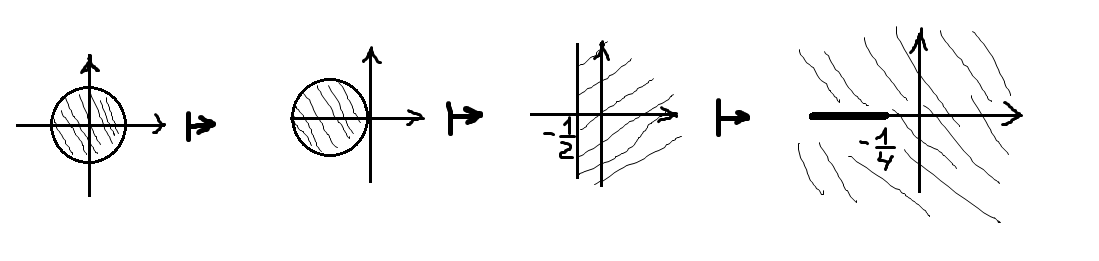
\includegraphics{Образ_Кебе.png}
		\caption{Картинка отображений после замен}
	\end{figure}
	Чтобы доказать частный случай гипотезы Бибербаха потребуется изучить второй вопрос. Пусть у нас есть аналитичная функция $f(z)$ в некоторой области $\Omega$. Тогда из замены переменной через Якобиан мы знаем площадь образа:
	$$S_{f(\Omega)}=\int\limits_{\Omega}|f^{'}(z)|^2d\lambda_2(z)$$
	Эта формула учитывает наложение образа на себя, поэтому честную площадь мы получим в случае однолистной функции.
	
	Рассмотрим однолистную функцию $f(z)=\displaystyle\sum_{n=0}^{+\infty}a_nz^n$ из единичного диска.
	$$S_{f(D)}=\int\limits_D|f^{'}(z)|^2d\lambda_2(z)=\int\limits_Df^{'}(z)\overline{f^{'}(z)}d\lambda_2(z)=\int\limits_D\left(\sum_{n=1}^{+\infty}na_nz^{n-1}\right)\left(\sum_{n=1}^{+\infty}n\overline{a_n}\overline{z}^{n-1}\right)d\lambda_2(z)=$$
	$$=\int_0^1\int_0^{2\pi}\left(\sum_{n=1}^{+\infty}na_n(re^{i\varphi})^{n-1}\right)\left(\sum_{n=1}^{+\infty}n\overline{a_n}(re^{-i\varphi})^{n-1}\right)rdrd\varphi$$
	$$=\int_0^{2\pi}\int_0^1\sum_{n=1}^{+\infty}n^2|a_n|^2r^{2n-2}rdrd\varphi=\pi\sum_{n=1}^{+\infty}n|a_n|^2$$
	Теперь если рассмотреть однолистную функцию в кольце $r<|z|<R$, то пишется та же выкладка и получаем:
	\begin{proposition}
		Для однолистной функции в единичном круге верна формула:
		$$S_{f(D)}=\pi\sum_{n=1}^{+\infty}n|a_n|^2$$
		Для однолистной функции в кольце $A:r<|z|<R$ верна формула:
		$$S_{f(A)}=\pi\sum_{-\infty}^{+\infty}n|a_n|^2(R^{2n}-r^{2n})$$
	\end{proposition}
	Заметим, что формулы положительны, как и полагается площади, а также не обязаны сходится, так как никто не гарантировал ограниченность образа.
	
	Теперь поговорим о симметричном случае, если так можно выразиться. Пусть функция однолистна во внешности некоторого шара с радиусом $r$, переводящая бесконечность в себя. Тут логично уметь считать площадь дополнения образа, назовем эту область $\Omega$. Во-первых, мы знаем, что такая функция раскладывается в ряд Лорана, при этом аналитичная часть будет включать в себя только полином первой степени. Нет старших членов из принципа аргумента из-за однолистности на бесконечности, а линейный есть, так как бесконечность неподвижная точка в рассматриваемом случае.
	$$f(z)=c_1z+c_0+\sum_{n=1}^{+\infty}c_{-n}z^{-n}$$
	\begin{figure}[H]
		\centering
		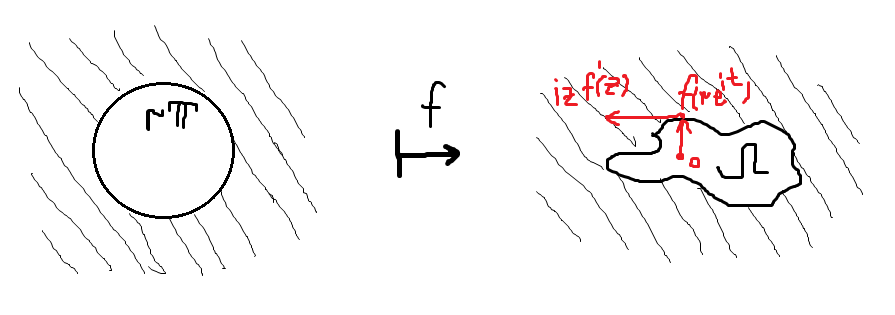
\includegraphics{Площадь_доп_однолистной.png}
		\caption{Поясняющая картинка}
	\end{figure}
	Формулу площади мы знаем:
	$$S_{f(\Omega)}=\int_0^{2\pi}\frac{r^2(t)}{2}d\varphi(t)$$
	$$r(t)=|f(re^{it}|\quad\varphi(t)=Im\,\log f(re^{it})$$
	$$dIm\,\log f(re^{it})=Im\left(\frac{f^{'}(re^{it}}{f(re^{it})}ire^{it}dt\right)=Re\left(\frac{zf^{'}(z)}{f(z)}\right)dt$$
	$$S_{f(\Omega)}=\int_0^{2\pi}\frac{f(z)\overline{f(z)}}{2}Re\left(\frac{zf^{'}(z)}{f(z)}\right)dt=\frac{1}{2}Re\,\int_0^{2\pi}zf^{'}(z)\overline{f(z)}dt$$
	
	Тем самым получаем следующее:
	\begin{proposition}
		Пусть функция $f(z)$ однолистна во внешности круга с радиусом $r$ и оставляет бесконечность на месте, а также не принимает значение 0 (это пожалуй самое важное), тогда верна формула площади:
		$$f(z)=c_1z+c_0+\sum_{n=1}^{+\infty}c_{-n}z^{-n}$$
		$$S_{f(\Omega)}=\pi\left(|c_1|r^2-\sum_{n=1}^{+\infty}\frac{n|c_{-n}|^2}{r^{2n}}\right)$$
	\end{proposition}
	\section{Однолистные функции: оценки на коэффициенты, симметризация и геометрический взгляд}
	Теперь мы наконец можем перейти к изучению устройства функций из класса $S$.
	\begin{definition}
		За класс $\Sigma$ обозначим множество однолистных функций в дополнении единичного круга: $\widehat{\Co}\setminus\overline{D}$ с дополнительными условиями $f(\infty)=\infty,\,f^{'}(\infty)=1$
	\end{definition}
	Их ряд соответственно выглядит так:
	$$f(z)=z+b_0+\sum_{n=1}^{+\infty}b_nz^{-n}$$
	Сразу можем получить:
	\begin{theorem}
		Для функции $f$ из класса $\Sigma$ верна оценка $|b_1|\leq 1$.
	\end{theorem}
	\begin{proof}
		Возьмем произвольное $r>1$ и посмотрим на площадь дополнения образа $\widehat{\Co}\setminus\overline{rD}$
		$$S_{\Omega_r}=\pi\left(r^2-\sum_{n=1}^{+\infty}\frac{n|b_n|^2}{r^{2n}}\right)>0$$
		Устремляя $r$ к 1, получаем требуемую оценку на коэффициент.
	\end{proof}
	Интересный вопрос о том, когда достигается максимум. Из доказательства видно, что если $|b_1|=1$, то последующие коэффициенты должны быть нулевыми, а тогда функция реализующая максимум это
	$$f(z)=z+c_0+\frac{e^{i\alpha}}{z}$$
	
	У нас есть два класса однолистных функций, которые имеют одинаковые условия и живут на похожих областях, значит наверное можно каким-то образом получить связь между этими классами, а так как области являются инверсными друг к другу, то мы сразу получаем преобразование функции из одного класса в другой, а именно:
	$$f(z)\in S\Rightarrow \frac{1}{f(\frac{1}{z})}\in\Sigma$$
	
	Заметим, что пользуясь оценкой для функции класса $\Sigma$ и этим преобразованием, мы не сможем доказать даже частный случай гипотезы Бибербаха, поэтому нужна еще какая-то теория.
	
	Есть такой способ - построить по одной однолистной функции другую. Зачем это нужно, кроме как интересно, узнаем на следующей лекции.
	
	Итак, пусть есть однолистная функция $f(z)$ в единичном круге, оставляющая 0 на месте. Тогда следующая функция тоже будет однолистна:
	$$g(z)=z\sqrt{\frac{f(z^2)}{z^2}}$$
	Разберемся с этим подорбнее. То что стоит под корнем не вызывает вопросов, кроме как в $z=0$, но и там нет проблем, так как мы требовали $f(0)=0$, а из-за квадрата аргумента функции получаем, что кратность 0 равна 2. Остается разобраться, что происходит при взятии корня. Если проверить на равенство $g(w)=g(z)$, то окажется, что $z^2=w^2$, поэтому либо числа совпали, либо отличаются на знак, но во втором случае возвращаясь к исходному определению $g$получим, что равенства не было. Также можно заметить, что функция нечетна.
	\begin{theorem}
		Если функция $g\in\Sigma,g\neq0$, то тогда $|b_0|\leq2$.
	\end{theorem}
	\begin{proof}
		$$g(z)=z+b_0+\sum_{n=1}^{+\infty}b_nz^{-n}$$
		$$h(z)=z\sqrt{\frac{g(z^2)}{z^2}}=z\sqrt{1+\frac{b_0}{z^2}+\frac{b_1}{z^4}+\cdots}=z+\frac{b_0}{2z}+\emph{младшие порядки}$$
		То есть получили функцию из класса $\Sigma$, а тогда мы знаем оценку на ее коэффициент при -1 степени, откуда получаем требуемое.
	\end{proof}
	Ну теперь наконец докажем слабую гипотезу Бибербаха.
	\begin{theorem}
		Если функция принадлежит классу $S$, то $|a_2|\leq2$.
	\end{theorem}
	\begin{proof}
		Переведем исходную функцию в функцию из класса $\Sigma$:
		$$g(z)=\frac{1}{f(\frac{1}{z})}$$
		Нетрудно проверить, что она действительно из нужного класса. Позанимаемся рядами...
		$$g(z)=\frac{1}{\frac{1}{z}+\frac{a_2}{z^2}+\cdots}=\frac{z}{1+\frac{a_2}{z}+\cdots}=z(1-\alpha+\alpha^2-\cdots),$$
		где $\alpha=\frac{a_2}{z}+\frac{a_3}{z^2}+\cdots$
		$$g(z)=z-a_2+\emph{младшие порядки}$$
		Тогда по предыдущей теореме получаем нужную оценку.
	\end{proof}
	И снова вопрос о достижении максимума. Если пройтись по пути доказательства теоремы, то видим, что максимум достигается тогда и только тогда, когда достигается максимум модуля свободного члена для функции из класса $\Sigma$, а этот максимум достигается тогда и только тогда, когда достигается максимум коэффициента при минус первой степени у функции из того же класса, а этот вопрос мы обсуждали и получали соответствующий вид функции. Так вот, мне лень делать преобразования для того вида, поэтому это упражнение для вас, а я просто пишу ответ: функции из класса Кебе.
	
	Можем сделать еще какие-то оценки. Мы знаем, что для функции $g\in\Sigma, g(z)\neq0$ выполнена формула (из формулы площади):
	$$g(z)=z+b_0+\sum_{n=1}^{+\infty}\frac{b_n}{z^n}\Rightarrow\sum_{n=1}^{+\infty}n|b_n|^2<1$$
	Тогда по КБШ можем сделать оценку:
	$$|g^{'}(z)|=\left|1-\sum_{n=1}^{+\infty}\frac{nb_n}{z^{n+1}}\right|\leq1+\sqrt{\sum_{n=1}^{+\infty}\frac{n}{|z|^{2(n+1)}}}\sqrt{\sum_{n=1}^{+\infty}n|b_n|^2}=1+\sqrt{\sum_{n=1}^{+\infty}\frac{n}{|z|^{2(n+1)}}}$$
	$$\sum_{n=1}^{+\infty}\frac{n}{r^{2n}}=\sum_{n=1}^{+\infty}n(r^{-2})^n=\frac{r^{-2}}{(1-r^{-2})^2}=\frac{r^2}{(1-r^2)^2}$$
	$$|g^{'}(z)|\leq\frac{|z|^2}{|z|^2-1}$$
	
	Еще немного оценок, но теперь геометрического характера. Мы знаем всякие разные оценки на коэффициенты функции из класса $\Sigma$ и понимаем как выглядит графически образ, но можно ли понять например на сколько большая или маленькая область не покроется? Например если взять функцию $f(z)=z$, то найдутся две непокрытые точки на расстоянии хотя бы 2. А если взять удвоенное преобразование Жуковского, то получим две непокрытые точки на расстоянии 4. Ну вот правильный ответ содержится в следующей:
	\begin{theorem}
		Если функция $f\in\Sigma,f(z)\neq0$, то расстояние между двумя непокрытыми точками образом функции не превосходит 4. А если функция $g\in\Sigma$, то найдутся хотя бы две непокрытые точки, расстояние между которыми хотя бы 2.
	\end{theorem}
	\begin{proof}
		Докажем первое утверждение. Пусть $h_1,h_2$ непокрытые точки. Так как можно сдвигать функцию на константу, то из оценки на модуль свободного члена получаем $|h_1-b_0|,|h_2-b_0|\leq2$, откуда по неравенству треугольника нужное неравенство.
		
		Вторая часть:
		$$g(z)=z+b_0+\sum_{n=1}^{+\infty}\frac{b_n}{z^n}$$
		Возьмем произвольное $r>1$, тогда получаем:
		$$r\cdot\max|g(re^{it})-g(-re^{it})|\geq\frac{1}{2\pi}\int_0^{2\pi}|g(re^{it})-g(-re^{it})|re^{-it}dt\geq\left|\int_0^{2\pi}[g(re^{it})-g(-re^{it})]re^{-it}dt\right|=2r^2,$$
		где последний переход из ортогональности. Устремляя $r$ к единице получаем, что найдутся две точки с границы, которые перейдут в две точки на границе образа (то есть непокрытые), расстояние между которыми 2.
	\end{proof}
	\section{Теорема об искажении и теорема Кёбе о четверти}
	С этим разделом я поступлю очень плохо и просто. Я его не затехаю. Мне просто сейчас, ну скажем кратко, хочется умереть.
	
	Если на сообщении с конспектом в телеге будет >20 дизлайков (кодовый для меня реакт, чтобы мне никто личку не засирал), то я собирусь с остатками того что осталось и затехаю и обновлю конспект до вечера 28.06.26 (до 20:00 условно, не позже). Я просто вообще сомневаюсь, что этот конспект будет читать ну хотя бы 5 человек.
	\begin{theorem}
		(Теорема об искажении) Для функции из класса $S$ выполняются:
		$$\frac{|z|}{(1+|z|)^2}\leq|f(z)|\leq\frac{|z|}{(1-|z|)^2}$$
		$$\frac{1-|z|}{(1+|z|)^3}\leq|f^{'}(z)|\leq\frac{1+|z|}{(1-|z|)^3}$$
	\end{theorem}
	\begin{proof}
		
	\end{proof}
	\begin{theorem}
		(Кёбе о четверти) Для функции из класса $S$ выволняется: $B_{\frac{1}{4}}(0)\subset f(B_1(0))$.
	\end{theorem}
	\begin{proof}
		
	\end{proof}
	\section{Класс Блоха}
	\begin{definition}
		Определим класс Блоха $\mathcal{B}$, как класс аналитичных функций в круге с ограниченной полунормой $||f||_{\mathcal{B}}:=\sup\limits_{z\in D}|f^{'}(z)|(1-|z|^2)<+\infty$.
	\end{definition}
	Иногда вместо этой полунормы берут в качестве эквивалентного определения норму $|f(0)|+\sup\limits_{z\in D}|f^{'}(z)|(1-|z|^2)$.
	Свойства данного класса:
	\begin{enumerate}
		\item Преобразования Мебиуса инвариантны в данном классе, так как очевидно сохраняют норму:
		$$g(z)=f(\Phi_a(z))\Rightarrow||g||=||f||$$
		\item $H^{\infty}(D)\subset\mathcal{B}$, так как из формулы Коши получаем:
		$$f^{'}(z)=\frac{1}{2\pi i}\oint\limits_{|w|=1}\frac{f(w)dw}{(w-z)^2}\Rightarrow|f^{'}(0)|\leq C$$
		А далее пересаживая 0 в произвольную точку круга Мебиусом получаем равномерную ограниченность производной в круге, а значит и полунорма Блоха ограничена.
		\item Следующий пример показывает, что равенства предыдущих классов нет, так как можно вспомнить однажды упоминаемую функцию Блоха или рассмотреть простые лакунарные ряды, но для начала бонус от меня про лакунарность:
		\begin{definition}
			Лакунарной функцией будем называть аналитичную в единичном круге функцию, которая не может быть продолжена ни за какой участок единичной окружности, а ее ряд Тейлора в 0 будем соответсвенно называть лакунарным рядом.
		\end{definition}
		\begin{theorem}
			(Адамара о лакунах) Рассмотрим функцию $f(z)=\sum_{n=1}^{+\infty}c_nz^{\lambda_n}$ у которой положительный радиус сходимости $r$ в 0, а $\{\lambda_n\}$ некоторая возрастающая последовательность натуральных чисел. Тогда если существует некоторое $\delta>0$, что $\frac{\lambda_{n+1}}{\lambda_n}>\delta$ для всех $n$, то $f(z)$ будет лакунарной.
		\end{theorem}
		Мы же рассмотрим частный случай, а именно пусть $0<q\in\mathbb{N}$. Тогда\\ $g(z)=\sum_{n=1}^{+\infty}z^{q^n}$ будет лакунарной (это мы давно показывали), а также будет лежать в классе Блоха. Действительно:
		$$\frac{|zg^{'}(z)|}{1-|z|}=\sum_{n=1}^{+\infty}q^n|z|^{q^n}\cdot\sum_{n=1}^{+\infty}|z|^n\leq\sum_{m=0}^{+\infty}\sum_{q^n\leq m}q^n|z|^m=\sum_{m=0}^{+\infty}\frac{q^{n_m}-1}{q-1}|z|^m\leq$$
		$$\leq\frac{q}{q-1}\sum_{m=0}^{+\infty}m|z|^m=\frac{q}{q-1}\frac{|z|}{(1-|z|)^2}$$
		То есть $|g^{'}(z)|(1-|z|^2)\leq\frac{q}{q-1}(1+|z|)$
		\item Если функция однолистна, то логарифм ее производной лежит в классе Блоха (определен, так как производная не 0). Это так, так как достаточно доказать это утверждение для функций из класса $S$, а тут мы знаем оценку модуля логарифма производной из док-ва теоремы об искажении (сами выше посмотрите), откуда даже бонусом получаем, что норма таких функций ограничена, внезапно, 6 (внезапно всмысле почему 6, а не другая константа типо $\pi$ или более логичного, хотя на целых функциях и не такие числовые фокусы были...).
		\item Если $f(z)=\displaystyle\sum_{n=0}^{+\infty}a_nz^n\in\mathcal{B}$ и п.в. имеет некасательный предел, то $|a_n|\rightarrow0$. Во-первых, есть формула Коши:
		$$a_n=\frac{1}{2\pi i}\frac{1}{n}\oint\limits_{\gamma}\frac{f^{'}(z)dz}{z^n}$$
		Давайте возьмем последовательность точек, которая сгущается к некоторой точке на границе круга, как в некасательном пределе, при этом радиусы очередных будут $1-\frac{1}{n}$. Тогда вспоминая значение числа $e$ через предел получаем оценку:
		$$|a_n|\leq \frac{e}{n}\sup\limits_{\theta_n}|f^{'}(r_ne^{i\theta_n})|$$
		Оценим модули производных в наших точках так: возьмем вокруг каждой $z_n=r_ne^{i\theta_n}$ круг радиуса $(Cn)^{-1}$, где константа общая и есть из некасательного предела (чтобы все это не вылезло за единичный круг и было в конусе из некасательного предела), тогда снова по Коши имеем:
		$$f^{'}(r_ne^{i\theta_n})=\frac{1}{2\pi i}\oint\limits_{\gamma_n}\frac{f(w)-f(e^{i\theta})}{(w-r_ne^{i\theta_n})^2}dw$$
		$$|f^{'}(r_ne^{i\theta_n})|\leq Cn\sup\limits_{w}|f(w)-f(e^{i\theta})|$$
		И супремум стремится к 0, так как у нас есть некасательный предел, а значит подставляя эту оценку производной в оценку коэффициента, получаем требуемое.
	\end{enumerate}
	\section{Бонус: философия экстремальных длин}
	Этого бонуса не будет, так как для экзамена не требуется, а автору уже совсем плохо живется...
	\newpage
	\section{Билеты}
	Коллеги, с прискорбием сообщаю вам, что закончился еще один замечальный курс лекций от Величайшего Юрия Сергеевича. Мне не удалось добиться большего числа лекций, я признаю поражение. Прилагаю ниже список билетов от Юрия Сергеевича.
	\begin{enumerate}
		\item Голоморфность и аналитичность. Уравнения Коши-Римана. Примеры.
		\item Дифференциальные формы. Точность и замкнутость. Теоремы о точных формах.
		\item Теорема Коши.
		\item Формула Коши. Лемма об устранимой особенности.
		\item Голоморфность равносильна аналитичности.
		\item Оператор Лапласа. Теорема о среднем.
		\item Теорема Лиувилля. Принцип максимума.
		\item Первообразная вдоль пути. Первообразная вдоль гомотопии.
		\item Функции аналитические в кольце. Разложение в ряд Лорана.
		\item Классификация изолированных особенностей. Теорема Сохоцкого.
		\item Теорема о вычетах. Подсчет интеграла $\frac{\sin t}{t}$
		\item Мероморфные функции. Вычет в бесконечноти. Характеризация рациональных функций.
		\item Принцип аргумента. Теорема Руше.
		\item Сходимость аналитичных функций. Сходимость производных.
		\item Лемма Шварца. Автоморфизмы круга.
		\item Теорема Монтеля.
		\item Однолистные функции. Сходимость однолистных функций.
		\item Теорема Римана. План доказательства. Примеры конформных отображений.
		\item Теорема Римана. Окончание доказательства.
		\item Принципы симметрии Римана-Шварца.
		\item Функция Жуковского. Конформное отображение на полосу.
		\item Отображение на прямоугольник. Эллиптический синус.
		\item Формулы Кристоффеля-Шварца. Примеры.
		\item Модулярная функция.
		\item Формула Пуассона в круге.
		\item Гармонические функции с ограниченным p-средними. Граничные значения при p>1.
		\item Граничные значения при p=1. Положительные гармонические функции. Неравенство Гарнака.
		\item Существование некасательных пределов.
		\item Произведения Бляшке. Сходимость. Примеры.
		\item Формула Пуассона-Йенсена.
		\item Граничные значения произведений Бляшке.
		\item Условие Бляшке для функций с ограниченным p-средним. Факторизация.
		\item Целые функции. Порядок и тип. Факторизация. Примеры.
		\item Порядок и тип целой функции через коэффициенты ряда Тейлора.
		\item Однолистные функции. Класс сигма. Формула площадей.
		\item Принцип симметризации для однолистных функций. Оценки на функции из класса сигма.
		\item Оценка на $a_2$
		\item Теорема об искажении. Теорема Кебе о четверти.
		\item Класс Блоха. Свойства.
	\end{enumerate}
\end{document}